% file: chap3.tex

\chapter{改进神经网络的学习方法}
\label{ch:ImprovingTheWayNeuralNetworksLearn}

当一个高尔夫球员刚开始学习打高尔夫时,他们通常会在挥杆的练习上花费大多数时间。慢
慢地他们才会在基本的挥杆上通过变化发展其他的击球方式,学习低飞球、左曲球和右曲球。
类似的,我们现在仍然聚焦在反向传播算法的理解上。这就是我们的“基本挥杆”,神经网络
中大部分工作学习和研究的基础。本章,我会解释若干技术能够用来提升我们关于%
\gls*{bp}的初级的实现,最终改进网络学习的方式。

本章涉及的技术包括:更好的\gls*{cost-func}的选择~——~%
\hyperref[sec:the_cross-entropy_cost_function]{交叉熵}\gls*{cost-func};四种称为%
\hyperref[sec:overfitting_and_regularization]{“\gls*{regularization}”的方法}(L1 和 L2 \gls*{regularization},
  \gls*{dropout}和训练数据的人为扩展),这会让我们的网络在训练集之外的数据上更好地泛化;%
\hyperref[sec:weight_initialization]{更好的\gls*{weight}初始化方法};还有%
\hyperref[sec:how_to_choose_a_neural_network's_hyper-parameters]{帮助选择好的超
  参数的启发式想法}。同样我也会再给出一些简要的%
\hyperref[sec:other_techniques]{其他技术介绍}。这些讨论之间的独立性比较大,所有
你们可以随自己的意愿挑着看。另外我还会在代码中%
\hyperref[sec:handwriting_recognition_revisited_the_code]{实现}这些技术,使用他
们来提高在\hyperref[ch:UsingNeuralNetsToRecognizeHandwrittenDigits]{第一章}中的
分类问题上的性能。

当然,我们仅仅覆盖了大量已经在神经网络中研究发展出的技术的一点点内容。从林林总总
的已有技术中入门的最佳策略,是深入研究一小部分最重要的,这是本书的观点。掌握了这
些关键技术不仅仅对这些技术本身的理解很有用,而且会深化你对使用神经网络时会遇到哪
些问题的理解。这会让你做好在需要时快速学会其他技术的充分准备。

\section{交叉熵代价函数}
\label{sec:the_cross-entropy_cost_function}

我们大多数人不喜欢被指出错误。在开始学习弹奏钢琴不久后,我在一个听众前做了处女秀。
我很紧张,开始时将八度音阶的曲段演奏得很低。我很困惑,因为不能继续演奏下去了,直
到有个人指出了其中的错误。当时,我非常尴尬。不过,尽管不开心,我们却能够因为明显
的犯错快速地学习到正确的东西。你应该相信下次我再演奏肯定会是正确的!相反,在我们
的错误不是很好地定义的时候,学习的过程会变得更加缓慢。

理想地,我们希望和期待神经网络可以从错误中快速地学习。在实践中,这种情况经常出现
吗?为了回答这个问题,让我们看看一个小例子。这个例子包含一个只有一个输入的神经元:

\begin{center}
  \includegraphics{tikz28}
\end{center}

我们会训练这个神经元来做一件非常简单的事:让输入 $1$ 转化为 $0$。当然,这很简单
了,手工找到合适的\gls*{weight}和\gls*{bias}就可以了,不需要什么学习算法。然而,
看起来使用梯度下降的方式来学习\gls*{weight}和\gls*{bias}是很有启发的。所以,我们
来看看神经元如何学习。

为了让这个例子更明确,我会首先将\gls*{weight}和\gls*{bias}初始化为 $0.6$ 和$0.9$。
这些就是一般的开始学习的选择,并没有任何刻意的想法。一开始的神经元的输出是
$0.82$,所以这离我们的目标输出 $0.0$ 还差得很远。从下图来看看神经元如何学习到让
输出接近 $0.0$ 的。注意这些图像实际上是正在进行梯度的计算,然后使用梯度更新来对%
\gls*{weight}和\gls*{bias}进行更新,并且展示结果。设置\gls*{learning-rate}
$\eta=0.15$ 进行学习一方面足够慢的让我们跟随学习的过程,另一方面也保证了学习的时
间不会太久,几秒钟应该就足够了。\gls*{cost-func}是我们在第一章用到的二次函数,$C$。这里
我也会给出准确的形式,所以不需要翻到前面查看定义了。
\begin{center}
  \includegraphics{saturation1-0}
\end{center}
随着\gls*{epoch}的增加,神经元的输出、\gls*{weight}、\gls*{bias}和代价的变化如下面
一系列图形所示:
\begin{center}
    \includegraphics{saturation1-50}\includegraphics{saturation1-100}\\
    \includegraphics{saturation1-150}\includegraphics{saturation1-200}\\
    \includegraphics{saturation1-250}\includegraphics{saturation1-300}
\end{center}

正如你所见,神经元快速地学到了使得\gls*{cost-func}下降的\gls*{weight}和\gls*{bias},给出
了最终的输出为 $0.09$。这虽然不是我们的目标输出 $0.0$,但是已经挺好了。假设我们
现在将初始\gls*{weight}和\gls*{bias}都设置为 $2.0$。此时初始输出为 $0.98$,这是
和目标值的差距相当大的。现在看看神经元学习的过程。
\begin{center}
  \includegraphics{saturation2-0}
\end{center}
你将看到如下的一系列变化:\label{saturation2_anchor}
\begin{center}
  \includegraphics{saturation2-50}\includegraphics{saturation2-100}\\
  \includegraphics{saturation2-150}\includegraphics{saturation2-200}\\
  \includegraphics{saturation2-250}\includegraphics{saturation2-300}
\end{center}

虽然这个例子使用的了同样的\gls*{learning-rate}($\eta=0.15$),我们可以看到刚开
始的学习速度是比较缓慢的。对前 $150$ 左右的学习次数,\gls*{weight}和\gls*{bias}
并没有发生太大的变化。随后学习速度加快,与上一个例子中类似了,神经网络的输出也迅
速接近 $0.0$。

这种行为看起来和人类学习行为差异很大。正如我在此节开头所说,我们通常是在犯错比较
明显的时候学习的速度最快。但是我们已经看到了人工神经元在其犯错较大的情况下其实学
习很有难度。而且,这种现象不仅仅是在这个小例子中出现,也会在更加一般的神经网络中
出现。为何学习如此缓慢?我们能够找到避免这种情况的方法吗?

为了理解这个问题的源头,想想我们的神经元是通过改变\gls*{weight}和\gls*{bias},并
以一个\gls*{cost-func}的偏导数($\partial C/\partial w$ 和 $\partial C/\partial b$)决定
的速度学习。所以,我们在说“学习缓慢”时,实际上就是说这些偏导数很小。理解他们为
何这么小就是我们面临的挑战。为了理解这些,让我们计算偏导数看看。我们一直在用的是
方程~\eqref{eq:6}表示的二次\gls*{cost-func},定义如下
\begin{equation}
  C = \frac{(y-a)^2}{2}
\label{eq:54}\tag{54}
\end{equation}

其中 $a$ 是神经元的输出,训练输入为 $x=1$,$y=0$ 则是目标输出。显式地使用%
\gls*{weight}和偏置来表达这个,我们有 $a = \sigma(z)$,其中 $z = wx+b$。使用链式
法则来求\gls*{weight}和\gls*{bias}的偏导数就有:
\begin{align}
  \frac{\partial C}{\partial w} &= (a-y)\sigma'(z) x = a \sigma'(z)\label{eq:55}\tag{55}\\
  \frac{\partial C}{\partial b} &= (a-y)\sigma'(z) = a \sigma'(z)\label{eq:56}\tag{56}
\end{align}

其中我已经将 $x = 1$ 和 $y = 0$ 代入了。为了理解这些表达式的行为,让我们仔细看
$\sigma'(z)$ 这一项。首先回忆一下 $\sigma$ 函数图像:
\begin{center}
  \includegraphics{sigmoid_function}
\end{center}

我们可以从这幅图看出,当神经元的输出接近 $1$ 的时候,曲线变得相当平,所以
$\sigma'(z)$ 就很小了。方程~\eqref{eq:55} 和~\eqref{eq:56} 也告诉我们 $\partial
C/\partial w$ 和 $\partial C/\partial b$ 会非常小。这其实就是学习缓慢的原因所在。
而且,我们后面也会提到,这种学习速度下降的原因实际上也是更加一般的神经网络学习缓
慢的原因,并不仅仅是在这个特例中特有的。

\subsection{引入交叉熵代价函数}
\label{sec:introducing_the_cross-entropy_cost_function}

那么我们如何解决这个问题呢?研究表明,我们可以通过使用交叉熵\gls*{cost-func}来替换二次代
价函数。为了理解什么是交叉熵,我们稍微改变一下之前的简单例子。假设,我们现在要训
练一个包含若干输入变量的的神经元,$x_1, x_2, \ldots$ 对应的\gls*{weight}为 $w_1,
w_2, \ldots$ 和\gls*{bias} $b$:

\begin{center}
  \includegraphics{tikz29}
\end{center}

神经元的输出就是 $a = \sigma(z)$,其中 $z = \sum_j w_j x_j+b$ 是输入的带权和。我
们如下定义这个神经元的交叉熵\gls*{cost-func}:
\begin{equation}
  C = -\frac{1}{n} \sum_x \left[y \ln a + (1-y ) \ln (1-a) \right]
\label{eq:57}\tag{57}
\end{equation}

其中 $n$ 是训练数据的总数,求和是在所有的训练输入 $x$ 上进行的,$y$ 是对应的目标
输出。

表达式~\eqref{eq:57} 是否解决学习缓慢的问题并不明显。实际上,甚至将这个定义看做
是\gls*{cost-func}也不是显而易见的!在解决学习缓慢前,我们来看看交叉熵为何能够解释成一个
\gls*{cost-func}。

将交叉熵看做是\gls*{cost-func}有两点原因。第一,它是非负的,$C > 0$。可以看出:(a)
\eqref{eq:57} 中的求和中的所有独立的项都是负数的,因为对数函数的定义域是 $(0,1)$;
      (b)求和前面有一个负号。

第二,如果对于所有的训练输入 $x$,神经元实际的输出接近目标值,那么交叉熵将接近
$0$\footnote{为了证明它我需要假设目标输出 $y$ 都是 $0$或$1$。这通常是解决分类问
  题的情况,例如,当计算布尔函数时。要了解当我们不做这个假设时会发生什么,看看在
  本节结束时的练习。}。假设在这个例子中,$y=0$ 而 $a\approx 0$。这是我们想要得到
的结果。我们看到公式 \eqref{eq:57} 中第一个项就消去了,因为 $y=0$,而第二项实际
上就是 $-\ln (1-a)\approx 0$。反之,$y=1$ 而 $a\approx 1$。所以在实际输出和目标
输出之间的差距越小,最终的交叉熵的值就越低了。

综上所述,交叉熵是非负的,在神经元达到很好的正确率的时候会接近 $0$。这些其实就是
我们想要的\gls*{cost-func}的特性。其实这些特性也是二次\gls*{cost-func}具备的。所以,交叉熵就是很
好的选择了。但是交叉熵\gls*{cost-func}有一个比二次\gls*{cost-func}更好的特性就是它避免了学习速度
下降的问题。为了弄清楚这个情况,我们来算算交叉熵函数关于\gls*{weight}的偏导数。
我们将 $a=\sigma(z)$ 代入到 \eqref{eq:57} 中应用两次链式法则,得到:
\begin{align}
  \frac{\partial C}{\partial w_j} &= -\frac{1}{n} \sum_x \left(
  \frac{y }{\sigma(z)} -\frac{(1-y)}{1-\sigma(z)} \right)
  \frac{\partial \sigma}{\partial w_j} \label{eq:58}\tag{58}\\
  &= -\frac{1}{n} \sum_x \left(
  \frac{y}{\sigma(z)}
  -\frac{(1-y)}{1-\sigma(z)} \right)\sigma'(z) x_j \label{eq:59}\tag{59}
\end{align}

将结果合并一下,简化成:
\begin{equation}
  \frac{\partial C}{\partial w_j} = \frac{1}{n} \sum_x \frac{\sigma'(z)
    x_j}{\sigma(z) (1-\sigma(z))} (\sigma(z)-y)
\label{eq:60}\tag{60}
\end{equation}

根据 $\sigma(z) = 1/(1+e^{-z})$ 的定义,和一些运算,我们可以得到 $\sigma'(z) =
\sigma(z)(1-\sigma(z))$。后面在练习中会要求你计算这个,现在可以直接使用这个结果。
我们看到 $\sigma'(z)$ 和 $\sigma(z)(1-\sigma(z))$ 这两项在方程中直接约去了,所以
最终形式就是:
\begin{equation}
  \frac{\partial C}{\partial w_j} =  \frac{1}{n} \sum_x x_j(\sigma(z)-y)
\label{eq:61}\tag{61}
\end{equation}

这是一个优美的公式。它告诉我们\gls*{weight}学习的速度受到 $\sigma(z)-y$,也就是
输出中的误差的控制。更大的误差,更快的学习速度。这是我们直觉上期待的结果。特别地,
这个\gls*{cost-func}还避免了像在二次\gls*{cost-func}中类似方程中 $\sigma'(z)$ 导致的学习缓慢,见
方程~\eqref{eq:55}。当我们使用交叉熵的时候,$\sigma'(z)$ 被约掉了,所以我们不再
需要关心它是不是变得很小。这种约除就是交叉熵带来的特效。实际上,这也并不是非常奇
迹的事情。我们在后面可以看到,交叉熵其实只是满足这种特性的一种选择罢了。

根据类似的方法,我们可以计算出关于\gls*{bias}的偏导数。我这里不再给出详细的过程,
你可以轻易验证得到
\begin{equation}
  \frac{\partial C}{\partial b} = \frac{1}{n} \sum_x (\sigma(z)-y)
\label{eq:62}\tag{62}
\end{equation}

再一次,这避免了二次\gls*{cost-func}中类似方程~\eqref{eq:56} 中 $\sigma'(z)$ 项导致的学习
缓慢。

\subsection*{练习}

\begin{itemize}
\item 验证 $\sigma'(z) = \sigma(z)(1-\sigma(z))$。
\end{itemize}

让我们重回最初的例子,来看看换成了交叉熵之后的学习过程。现在仍然按照前面的参数配
置来初始化网络,开始\gls*{weight}为 $0.6$,而\gls*{bias}为 $0.9$。
\begin{center}
  \includegraphics{saturation3-0}
\end{center}
看看在换成交叉熵之后网络的学习情况,你将看到如下变化的曲线:
\begin{center}
  \includegraphics{saturation3-50}\includegraphics{saturation3-100}\\
  \includegraphics{saturation3-150}\includegraphics{saturation3-200}\\
  \includegraphics{saturation3-250}\includegraphics{saturation3-300}
\end{center}

毫不奇怪,在这个例子中,神经元学习得相当出色,跟之前差不多。现在我们再看看之前出
问题的那个例子(\hyperref[saturation2_anchor]{链接}),\gls*{weight}和%
\gls*{bias}都初始化为$2.0$:
\begin{center}
  \includegraphics{saturation4-0}
\end{center}
你将看到如下变化的曲线:
\begin{center}
  \includegraphics{saturation4-50}\includegraphics{saturation4-100}\\
  \includegraphics{saturation4-150}\includegraphics{saturation4-200}\\
  \includegraphics{saturation4-250}\includegraphics{saturation4-300}
\end{center}

成功了!这次神经元的学习速度相当快,跟我们预期的那样。如果你观测的足够仔细,你可
以发现\gls*{cost-func}曲线要比二次\gls*{cost-func}训练前面部分要陡很多。那个交叉熵导致的陡度让我
们高兴,这正是我们期待的当神经元开始出现严重错误时能以最快速度学习。

我还没有提及刚才的示例用了什么\gls*{learning-rate}。刚开始使用二次\gls*{cost-func}的时候,
我们使用了 $\eta = 0.15$。在新例子中,我们还应该使用同样的\gls*{learning-rate}吗?
实际上,根据不同的\gls*{cost-func},我们不能够直接去套用同样的\gls*{learning-rate}。这好
比苹果和橙子的比较。对于这两种\gls*{cost-func},我只是通过简单的实验来找到一个能够让我们
看清楚变化过程的\gls*{learning-rate}的值。尽管我不愿意提及,但如果你仍然好奇,这
个例子中我使用了 $\eta = 0.005$。

你可能会反对说,上面\gls*{learning-rate}的改变使得上面的图失去了意义。谁会在意当%
\gls*{learning-rate}的选择是任意挑选的时候神经元学习的速度?!这样的反对其实没有
抓住重点。上面的图例不是想讨论学习的绝对速度。而是想研究学习速度的变化情况。

特别地,当我们使用二次\gls*{cost-func}时,学习在神经元犯了明显的错误的时候却比学习快接近
真实值的时候缓慢;而使用交叉熵学习正是在神经元犯了明显错误的时候速度更快。特别地,
当我们使用二次\gls*{cost-func}时,当神经元在接近正确的输出前犯了明显错误的时候,学习变得%
\textbf{更加缓慢};而使用交叉熵,在神经元犯明显错误时学习得更快。这些现象并不依
赖于如何设置\gls*{learning-rate}。

我们已经研究了一个神经元的交叉熵。不过,将其推广到有很多神经元的多层神经网络上也
是很简单的。特别地,假设 $y = y_1, y_2, \ldots$ 是输出神经元上的目标值,而
$a^L_1, a^L_2, \ldots$ 是实际输出值。那么我们定义交叉熵如下
\begin{equation}
  C = -\frac{1}{n} \sum_x \sum_j \left[y_j \ln a^L_j + (1-y_j) \ln (1-a^L_j) \right]
  \label{eq:63}\tag{63}
\end{equation}

除了这里需要对所有输出神经元进行求和 $\sum_j$ 外,这个其实和我们早前的公
式~\eqref{eq:57} 是一样的。这里不会给出一个推算的过程,但需要说明的是使用公
式~\eqref{eq:63} 确实会在很多的神经网络中避免学习的缓慢。如果你感兴趣,你可以尝
试一下下面问题的推导。

那么我们应该在什么时候用交叉熵来替换二次\gls*{cost-func}?实际上,如果在输出神经元是%
\gls*{sigmoid-neuron}时,交叉熵一般都是更好的选择。为什么?考虑一下我们初始化网
络的\gls*{weight}和\gls*{bias}的时候通常使用某种随机方法。可能会发生这样的情况,
这些初始选择会对某些训练输入误差相当明显~——~比如说,目标输出是 $1$,而实际值是
$0$,或者完全反过来。如果我们使用二次\gls*{cost-func},那么这就会导致学习速度的下降。它
并不会完全终止学习的过程,因为这些\gls*{weight}会持续从其他的样本中进行学习,但
是显然这不是我们想要的效果。

\subsection*{练习}

\begin{itemize}
\item 一个小问题就是刚接触交叉熵时,很难一下子记住那些诸如 $y$ 和 $a$ 的表达式对
  应的角色。又比如说,表达式的正确形式是 $-[y \ln a + (1-y) \ln (1-a)]$ 还是
  $-[a \ln y + (1-a) \ln (1-y)]$。在 $y=0$ 或者 $1$ 的时候第二个表达式的结果怎样?
  这个问题会困扰第一个表达式吗?为什么?
\item 在对单个神经元讨论中,我们指出如果对所有的训练数据有 $\sigma(z) \approx y$,
  交叉熵会很小。这个论断其实是和 $y$ 只是等于 $1$ 或者 $0$ 有关。这在分类问题一
  般是可行的,但是对其他的问题(如回归问题)$y$ 可以取 $0$ 和 $1$ 之间的中间值的。
  证明,交叉熵对所有训练输入在 $\sigma(z) = y$ 时仍然是最小化的。此时交叉熵的表
  示是:
  \begin{equation}
    C = -\frac{1}{n} \sum_x [y \ln y+(1-y) \ln(1-y)]
    \label{eq:64}\tag{64}
  \end{equation}
  而其中 $-[y \ln y+(1-y)\ln(1-y)]$ 有时候被称为%
  \href{http://en.wikipedia.org/wiki/Binary_entropy_function}{二元熵}。
\end{itemize}

\subsection*{问题}

\begin{itemize}
\item \textbf{多层多神经元网络}\quad 用%
  \hyperref[ch:HowTheBackpropagationAlgorithmWorks]{上一章}的定义符号,证明对二
  次\gls*{cost-func},关于输出层的\gls*{weight}的偏导数为
  \begin{equation}
    \frac{\partial C}{\partial w^L_{jk}} = \frac{1}{n}
    \sum_x a^{L-1}_k  (a^L_j-y_j) \sigma'(z^L_j)
    \label{eq:65}\tag{65}
  \end{equation}
  项 $\sigma'(z^L_j)$ 会在一个输出神经元困在错误值时导致学习速度的下降。证明对于
  交叉熵\gls*{cost-func},针对一个训练样本 $x$ 的输出误差 $\delta^L$为
  \begin{equation}
    \delta^L = a^L-y
    \label{eq:66}\tag{66}
  \end{equation}
  使用这个表达式来证明关于输出层的\gls*{weight}的偏导数为
  \begin{equation}
    \frac{\partial C}{\partial w^L_{jk}} = \frac{1}{n} \sum_x
    a^{L-1}_k  (a^L_j-y_j)
    \label{eq:67}\tag{67}
  \end{equation}
  这里 $\sigma'(z^L_j)$ 就消失了,所以交叉熵避免了学习缓慢的问题,不仅仅是在一个
  神经元上,而且在多层多元网络上都起作用。这个分析过程稍作变化对\gls*{bias}也是一样的。
  如果你对这个还不确定,那么请仔细研读一下前面的分析。
\item \textbf{在输出层使用线性神经元时使用二次\gls*{cost-func}}\quad 假设我们有一个多层
  多神经元网络,最终输出层的神经元都是\textbf{线性神经元},输出不再是 \gls*{sigmoid-func}作
  用的结果,而是 $a^L_j = z^L_j$。证明如果我们使用二次\gls*{cost-func},那么对单个训练样
  本 $x$ 的输出误差就是
  \begin{equation}
    \delta^L = a^L-y
    \label{eq:68}\tag{68}
  \end{equation}
  类似于前一个问题,使用这个表达式来证明关于输出层的\gls*{weight}和\gls*{bias}的
  偏导数为
  \begin{align}
    \frac{\partial C}{\partial w^L_{jk}} &= \frac{1}{n} \sum_x
                                           a^{L-1}_k  (a^L_j-y_j) \label{eq:69}\tag{69}\\
    \frac{\partial C}{\partial b^L_{j}} &= \frac{1}{n} \sum_x
                                          (a^L_j-y_j) \label{eq:70}\tag{70}
  \end{align}
  这表明如果输出神经元是线性的那么二次\gls*{cost-func}不再会导致学习速度下降的问题。在此
  情形下,二次\gls*{cost-func}就是一种合适的选择。
\end{itemize}

\subsection{使用交叉熵来对 MNIST 数字进行分类}

交叉熵很容易作为使用梯度下降和反向传播方式进行模型学习的一部分来实现。我们将会在
% \hyperref[sec:handwriting_recognition_revisited_the_code]{这一章的后面}进行对%
\hyperref[sec:implementing_our_network_to_classify_digits]{前面的程序}
\lstinline!network.py! 的改进。新的程序写在 \lstinline!network2.py!  中,不仅使
用了交叉熵,还有本章中介绍的其他的技术\footnote{代码可从
  \href{https://github.com/mnielsen/neural-networks-and-deep-learning/blob/master/src/network2.py}{GitHub}
  获取。}。现在我们看看新的程序在进行 MNIST 数字分类问题上的表现。如在第一章中那
样,我们会使用一个包含 $30$ 个隐藏元的网络,而\gls*{mini-batch}的大小也设置为
$10$。我们将\gls*{learning-rate}设置为 $\eta=0.5$ \footnote{在第一章里我们用了二
  次代价和 $\eta = 3.0$ 的\gls*{learning-rate}。上面已经讨论过,准确地说出当代价
  函数改变时用“相同的”学习速率意味什么,这是不可能的。对于两种\gls*{cost-func},在给出其
  它超参数的选择后,我都做了实验来找出一个接近优化性能的\gls*{learning-rate},顺
  便提一下,有一个非常粗略的将交叉熵和二次代价的\gls*{learning-rate}联系起来的推
  导。正如我们之前看到的,二次代价的梯度项中有一个额外的 $\sigma' =
  \sigma(1-\sigma)$。假设我们把这按照 $\sigma$ 的值平均,$\int_0^1 d\sigma
  \sigma(1-\sigma) = 1/6$。我们(非常粗略地)看到二次代价对于相同的%
  \gls*{learning-rate},以平均慢 $6$ 倍的速度进行学习。这提示我们一个合理的起点
  是把二次代价的\gls*{learning-rate}除以 $6$。当然,这个理由非常不严谨,不应被认
  真对待。不过,有时候这是个有用的起点。} 然后训练 $30$ 个\gls*{epoch}。
\lstinline!network2.py! 的接口和 \lstinline!network.py! 稍微不同,但是过程还是很
清楚的。你可以使用如 \lstinline!help(network2.Network.SGD)! 这样的命令来查看
\lstinline!network2.py! 的接口文档。

\begin{lstlisting}[language=Python]
>>> import mnist_loader
>>> training_data, validation_data, test_data = \
... mnist_loader.load_data_wrapper()
>>> import network2
>>> net = network2.Network([784, 30, 10], cost=network2.CrossEntropyCost)
>>> net.large_weight_initializer()
>>> net.SGD(training_data, 30, 10, 0.5, evaluation_data=test_data,
... monitor_evaluation_accuracy=True)
\end{lstlisting}

注意看下,\lstinline!net.large_weight_initializer()! 命令使用和第一章介绍的同样
的方式来进行\gls*{weight}和\gls*{bias}的初始化。我们需要运行这个命令,是因为我们
要在这一章的后面才改变默认的\gls*{weight}初始化命令。运行上面的代码我们得到了一
个 95.49\% 准确率的网络。这跟我们在第一章中使用二次\gls*{cost-func}得到的结果相当接近了,
95.42\%。

同样也来试试使用 $100$ 个隐藏神经元,交叉熵及其他参数保持不变的情况。在这个情形
下,我们获得了 96.82\% 的准确率。相比第一章使用二次\gls*{cost-func}的结果 96.59\%,这有
一定的提升。这看起来是一个小小的变化,但是考虑到误差率已经从 3.41\% 下降到3.18\%
了。我们已经消除了原误差的 $1/14$。这其实是可观的改进。

令人振奋的是交叉熵\gls*{cost-func}给了我们和二次代价相比类似的或者更好的结果。然而,这些
结果并没有能够明确地证明交叉熵是更好的选择。原因在于我花费了少许努力在选择诸如学
习速率,\gls*{mini-batch}大小等等这样的超参数上。为了让这些提升更具说服力,我们
需要对超参数进行深度的优化。然而,这些结果仍然是令人鼓舞的,巩固了我们早先关于交
叉熵优于二次代价的理论论断。

这只是本章后面的内容和整本书剩余内容中的更为一般的模式的一部分。我们将给出一个新
的技术,然后进行尝试,随后获得“提升的”结果。当然,看到这些进步是很好的。但是这些
提升的解释一般来说都困难重重。它们只有在我们进行了大量工作来优化所有其他的超参数
时,才确实具有说服力。工作量很大,需要大量的计算能力,我们通常也不会进行这样彻底
的调研。相反,我采用上面进行的那些不正式的测试来达成目标。然而你要记住这样的测试
仍然缺乏权威的证明,需要注意那些使得论断失效的迹象。

至此,我们已经花了大量篇幅介绍交叉熵。为何对一个只能给我们的 MNIST 结果带来一点
点性能提升的技术花费这么多的精力?后面,我们会看到其他的技术~——~%
\hyperref[sec:overfitting_and_regularization]{\gls*{regularization}},会带来更大的提升效果。所
以为何要这么细致地讨论交叉熵?部分原因在于交叉熵是一种广泛使用的\gls*{cost-func},值得深
入理解。但是更加重要的原因是神经元的饱和是神经网络中一个关键的问题,整本书都会不
断回归到这个问题上。因此我现在深入讨论交叉熵就是因为这是一种开始理解神经元饱和以
及如何解决这个问题的很好的实验。

\subsection{交叉熵的含义?源自哪里?}

我们对于交叉熵的讨论聚焦在代数分析和代码实现。这虽然很有用,但是也留下了一个未能
回答的更加宽泛的概念上的问题,如:交叉熵究竟表示什么?存在一些直觉上的思考交叉熵
的方法吗?我们如何想到这个概念?

让我们从最后一个问题开始回答:什么能够激发我们想到交叉熵?假设我们发现学习速度下
降了,并理解其原因是因为在公式~\eqref{eq:55} 和~\eqref{eq:56} 中的 $\sigma'(z)$
那一项。在研究了这些公式后,我们可能就会想到选择一个不包含 $\sigma'(z)$ 的代价函
数。所以,这时候对一个训练样本 $x$,其代价 $C = C_x$ 满足:
\begin{align}
  \frac{\partial C}{\partial w_j} &= x_j(a-y) \label{eq:71}\tag{71}\\
  \frac{\partial C}{\partial b } &= (a-y) \label{eq:72}\tag{72}
\end{align}

如果我们选择的\gls*{cost-func}满足这些条件,那么它们就能以简单的方式呈现这样的特性:初始
误差越大,神经元学习得越快。这也能够解决学习速度下降的问题。实际上,从这些公式开
始,现在我们就看看凭着我们数学的直觉推导出交叉熵的形式是可行的。我们来推一下,由
链式法则,我们有
\begin{equation}
  \frac{\partial C}{\partial b} = \frac{\partial C}{\partial a}
  \sigma'(z)
  \tag{73}
\end{equation}

使用 $\sigma'(z) = \sigma(z)(1-\sigma(z)) = a(1-a)$,上个等式就变成
\begin{equation}
  \frac{\partial C}{\partial b} = \frac{\partial C}{\partial a}
  a(1-a)
  \label{eq:74}\tag{74}
\end{equation}

对比等式~\eqref{eq:72},我们有
\begin{equation}
  \frac{\partial C}{\partial a} = \frac{a-y}{a(1-a)}
  \label{eq:75}\tag{75}
\end{equation}

对此方程关于 $a$ 进行积分,得到
\begin{equation}
  C = -[y \ln a + (1-y) \ln (1-a)]+ {\rm constant}
  \label{eq:76}\tag{76}
\end{equation}
其中 {\rm constant} 是积分常量。这是一个单独的训练样本 $x$ 对\gls*{cost-func}的贡献。为
了得到整个的\gls*{cost-func},我们需要对所有的训练样本进行平均,得到了
\begin{equation}
  C = -\frac{1}{n} \sum_x [y \ln a +(1-y) \ln(1-a)] + {\rm constant}
  \label{eq:77}\tag{77}
\end{equation}
而这里的常量就是所有单独的常量的平均。所以我们看到方程~\eqref{eq:71}
和~\eqref{eq:72} 唯一确定了交叉熵的形式,并加上了一个常量的项。这个交叉熵并不是
凭空产生的。而是一种我们以自然和简单的方法获得的结果。

那么交叉熵直觉含义又是什么?我们如何看待它?深入解释这一点会将我们带到一个不大愿
意讨论的领域。然而,还是值得提一下,有一种源自信息论的解释交叉熵的标准方式。粗略
地说,交叉熵是“不确定性”的一种度量。特别地,我们的神经元想要计算函数 $x
\rightarrow y = y(x)$。但是,它用函数 $x \rightarrow a = a(x)$ 进行了替换。假设
我们将 $a$ 想象成我们神经元估计为 $y = 1$ 的概率,而 $1-a$ 则是 $y=0$ 的概率。那
么交叉熵衡量我们学习到 $y$ 的正确值的平均起来的不确定性。 如果输出我们期望的结果,
不确定性就会小一点;反之,不确定性就大一些。当然,我这里没有严格地给出“不确定性”
到底意味着什么,所以看起来像在夸夸其谈。但是实际上,在信息论中有一种准确的方式来
定义不确定性究竟是什么。不过,我也不清楚在网络上,哪里有好的、短小的、包含有对这
个主题的讨论。但如果你要深入了解的话,维基百科包含一个%
\href{http://en.wikipedia.org/wiki/Cross_entropy#Motivation}{简短的总结},这会指
引你正确地探索这个领域。而更加细节的内容,你们可以阅读
\href{http://books.google.ca/books?id=VWq5GG6ycxMC}{Cover and Thomas} 的第五章涉
及 Kraft 不等式的有关信息论的内容。

\subsection*{问题}

\begin{itemize}
\item 我们已经深入讨论了使用二次\gls*{cost-func}的网络中在输出神经元饱和时候学习缓慢的问
  题,另一个可能会影响学习的因素就是在方程~\eqref{eq:61} 中的 $x_j$ 项。由于此项,
  当输入 $x_j$ 接近 $0$ 时,对应的\gls*{weight} $w_j$ 会学习得相当缓慢。解释为何
  不可以通过改变\gls*{cost-func}来消除 $x_j$ 项的影响。
\end{itemize}

\subsection{柔性最大值}
\label{subsec:softmax}

本章,我们大多数情况会使用交叉熵来解决学习缓慢的问题。但是,我希望简要介绍一下另
一种解决这个问题的方法,基于\textbf{\gls{softmax}}神经元层。我们不会实际在剩下的
章节中使用\gls*{softmax}层,所以你如果赶时间,就可以跳到下一个小节了。不过,%
\gls*{softmax}仍然有其重要价值,一方面它本身很有趣,另一方面,因为我们会在%
\hyperref[ch:Deeplearning]{第六章}在对深度神经网络的讨论中使用\gls*{softmax}层。

\gls*{softmax}的想法其实就是为神经网络定义一种新式的输出层。开始时和 S 型层一样
的,首先计算带权输入\footnote{在描述\gls*{softmax}的过程中我们会经常使用%
\hyperref[ch:HowTheBackpropagationAlgorithmWorks]{上一章}中介绍的符号。如果你需
要回想下那些符号,你可能需要看下那一章。} $z^L_j = \sum_{k} w^L_{jk} a^{L-1}_k +
  b^L_j$。不过,这里我们不会使用\gls*{sigmoid-func}来获得输出。而是,会在这一层
  上应用一种叫做\text{\gls{softmax-func}}在 $z^L_j$ 上。根据这个函数,第 $j$ 个
  神经元的激活值 $a^L_j$ 就是
\begin{equation}
  a^L_j = \frac{e^{z^L_j}}{\sum_k e^{z^L_k}}
  \label{eq:78}\tag{78}
\end{equation}
其中,分母中的求和是在所有的输出神经元上进行的。

如果你不熟悉这个\gls*{softmax-func},方程~\eqref{eq:78} 可能看起来会比较难理解。
因为对于使用这个函数的原因你不清楚。这能帮我们解决学习缓慢的问题也不明显。为了更
好地理解方程~\eqref{eq:78},假设我们有一个包含四个输出神经元的神经网络,对应四个
带权输入,表示为 $z^L_1, z^L_2, z^L_3$ 和 $z^L_4$。下面的例子中的条块显示带权输
入的可取值,和对应输出激活值的图形。要探索它,一个好的开始的地方是增加 $z^L_4$:
\begin{center}
  \includegraphics{softmax}
\end{center}

当你增加 $z^L_4$ 的时候,你可以看到对应激活值 $a^L_4$ 的增加,而其他的激活值就在
下降。例如下图显示 $z^L_4$ 为 $2$ 时:
\begin{center}
  \includegraphics{softmax-1}
\end{center}

下图显示 $z^L_4$ 为 $5$ 时:
\begin{center}
  \includegraphics{softmax-2}
\end{center}

类似地,如果你降低 $z^L_4$ 那么 $a^L_4$ 就随之下降,而其它激活值则增加。例如下图
显示 $z^L_4$ 为 $-2$ 时:
\begin{center}
  \includegraphics{softmax-3}
\end{center}

下图显示 $z^L_4$ 为 $-5$ 时:
\begin{center}
  \includegraphics{softmax-4}
\end{center}

实际上,如果你仔细看,你会发现在两种情形下,其他激活值的整个改变恰好填补
了 $a^L_4$的变化的空白。原因很简单,根据定义,输出的激活值加起来正好为 $1$,使用
公式~\eqref{eq:78} 我们可以证明:
\begin{equation}
  \sum_j a^L_j = \frac{\sum_j e^{z^L_j}}{\sum_k e^{z^L_k}} = 1
  \label{eq:79}\tag{79}
\end{equation}

所以,如果 $a^L_4$ 增加,那么其他输出激活值肯定会总共下降相同的量,来保证所有激活
值的和为 $1$。当然,类似的结论对其他的激活值也需要满足。

方程~\eqref{eq:78} 同样保证输出激活值都是正数,因为指数函数是正的。将这两点结合起
来,我们看到柔性最大值层的输出是一些相加为 $1$ 正数的集合。换言之,柔性最大值层的
输出可以被看做是一个概率分布。

这样的效果很令人满意。在很多问题中,能够将输出激活值 $a^L_j$ 理解为网络对于正确输
出为 $j$ 的概率的估计是非常方便的。所以,比如在 MNIST 分类问题中,我们可以
将 $a^L_j$ 解释成网络估计正确数字分类为 $j$ 的概率。

对比一下,如果输出层是 S 型层,那么我们肯定不能假设激活值形成了一个概率分布。我不
会证明这一点,但是源自 S 型层的激活值是不能够形成一种概率分布的一般形式的。所以使
用 S 型输出层,我们没有这样一个关于输出激活值的简单解释。

\subsection*{练习}

\begin{itemize}
\item 构造例子表明在使用 S 型输出层的网络中输出激活值 $a^L_j$ 的和并不会确保为
  $1$。
\end{itemize}

我们现在开始体会到柔性最大值函数的形式和行为特征了。来回顾一下:在公
式~\eqref{eq:78} 中的指数确保了所有的输出激活值是正数。然后方程~\eqref{eq:78} 中
分母的求和又保证了\gls*{softmax}的输出和为 $1$。所以这个特定的形式不再像之前那样
难以理解了:反而是一种确保输出激活值形成一个概率分布的自然的方式。你可以将其想象
成一种重新调节 $z^L_j$ 的方法,然后将这个结果整合起来构成一个概率分布。

\subsection*{练习}

\begin{itemize}
\item \textbf{\gls*{softmax}的单调性}\quad 证明如果 $j=k$ 则 $\partial a^L_j /
  \partial z^L_k$ 为正,$j \neq k$ 时为负。结果是,增加 $z^L_j$ 会提高对应的输出
  激活值 $a^L_j$ 并降低其他所有输出激活值。我们已经在滑动条示例中实验性地看到了
  这一点,这里需要你给出一个严格证明。
\item \textbf{\gls*{softmax}的非局部性}\quad S 型层的一个好处是输出 $a^L_j$ 是对
  应带权输入 $a^L_j = \sigma(z^L_j)$ 的函数。解释为何对于\gls*{softmax}层来说,
  并不是这样的情况:任何特定的输出激活值 $a^L_j$ 依赖\textbf{所有的}带权输入。
\end{itemize}

\subsection*{问题}

\begin{itemize}
\item \textbf{逆转\gls*{softmax}层}\quad 假设我们有一个使用\gls*{softmax}输出层
  的神经网络,然后激活值 $a^L_j$ 已知。证明对应带权输入的形式为 $z^L_j = \ln
  a^L_j + C$,其中常量 $C$ 是独立于 $j$ 的。
\end{itemize}

\textbf{学习缓慢问题:} 我们现在已经对柔性最大值神经元层有了一定的认识。但是我们
还没有看到一个柔性最大值层会怎么样解决学习缓慢问题。为了理解这点,让我们先定义一
个\textbf{\gls{log-likelihood}}\gls*{cost-func}。我们使用 $x$ 表示网络的训练输入,$y$ 表
示对应的目标输出。然后关联这个训练输入的\gls*{log-likelihood}\gls*{cost-func}就是
\begin{equation}
  C \equiv -\ln a^L_y
  \label{eq:80}\tag{80}
\end{equation}
所以,如果我们训练的是 MNIST 图像,输入为 $7$ 的图像,那么对应的%
\gls*{log-likelihood}代价就是 $-\ln a_7^L$。看看这个直觉上的含义,想想当网络表现
很好的时候,也就是确认输入为 $7$ 的时候。这时,他会估计一个对应的概率 $a_7^L$ 跟
$1$ 非常接近,所以代价 $-\ln a_7^L$ 就会很小。反之,如果网络的表现糟糕时,概率
$a_7^L$ 就变得很小,代价 $-\ln a_7^L$ 随之增大。所以对数似然\gls*{cost-func}也是满足我们
期待的\gls*{cost-func}的条件的。

那关于学习缓慢问题呢?为了分析它,回想一下学习缓慢的关键就是量 $\partial C /
\partial w^L_{jk}$ 和 $\partial C / \partial b^L_j$ 的变化情况。我不会显式地给出
详细的推导~——~我会在下面的问题中要求你们完成推导~——~但是通过一点代数运算你会得
到\footnote{注意这里的表示上的差异,这里的 $y$ 和上一段中的不同。在上一段中我们
  用 $y$ 来表示网络的目标输出,例如,如果输入是 7 的图像输出一个 $7$。但是接下来
  的方程中,我用 $y$ 表示对应于 $7$ 的输出激活值的向量,即,它是一个除了
  第 7 位为 $1$,其它所有位都是 $0$ 的向量。}:
\begin{align}
  \frac{\partial C}{\partial b^L_j} &= a^L_j-y_j \label{eq:81}\tag{81}\\
  \frac{\partial C}{\partial w^L_{jk}} &= a^{L-1}_k (a^L_j-y_j) \label{eq:82}\tag{82}
\end{align}

这些方程其实和我们前面对交叉熵得到的类似。就拿方程~\eqref{eq:82} 和~\eqref{eq:67}比
较。尽管后者我对整个训练样本进行了平均,不过形式还是一致的。而且,正如前面的分析,
这些表达式确保我们不会遇到学习缓慢的问题。事实上,把一个具有%
\gls*{log-likelihood}代价的\gls*{softmax}输出层,看作与一个具有交叉熵代价的 S 型
输出层非常相似,这是很有用的。

有了这样的相似性,你应该使用一个具有交叉熵代价的 S 型输出层,还是一个具有对数似然
代价的柔性最大值输出层呢?实际上,在很多应用场景中,这两种方式的效果都不错。本章
剩下的内容,我们会使用一个 S 型输出层和交叉熵代价的组合。后面,
在\hyperref[ch:Deeplearning]{第六章}中,我们有时候会使用柔性最大值输出层和对数似
然代价的组合。切换的原因就是为了让我们的网络和某些在具有影响力的学术论文中的形式
更为相似。作为一种更加通用的视角,柔性最大值加上对数似然的组合更加适用于那些需要
将输出激活值解释为概率的场景。那并不总是一个需要关注的问题,但是在诸如 MNIST 这种
有着不重叠的分类问题上确实很有用。

\subsection*{问题}

\begin{itemize}
\item 推导方程~\eqref{eq:81} 和~\eqref{eq:82}
\item \textbf{柔性最大值这个名称从何处来?}\quad 假设我们改变一下柔性最大值函数,
  使得输出激活值定义如下
  \begin{equation}
    a^L_j = \frac{e^{c z^L_j}}{\sum_k e^{c z^L_k}}
    \label{eq:83}\tag{83}
  \end{equation}
  其中 $c$ 是正的常量。注意 $c=1$ 对应标准的柔性最大值函数。但是如果我们使用不同
  的 $c$ 得到不同的函数,其本质上和原来的柔性最大值函数是很相似的。特别地,证明
  输出激活值也会形成一个概率分布,正如通常的柔性最大值函数。假设我们允许 $c$ 足
  够大,比如说 $c\rightarrow \infty$。那么输出激活值 $a_j^L$ 的极限值是什么?在
  解决了这个问题后,你应该能够清楚为什么我们把 $c=1$ 对应的函数看作是一个最大化
  函数的变柔和的版本。这就是柔性最大值术语的来源。
\item \textbf{柔性最大值和对数似然的\gls*{bp}}\quad 上一章,我们推导了使用 S 型层
  的\gls*{bp}算法。为了应用在柔性最大值层的网络上,我们需要搞清楚最后一层上误差的
  表示 $\delta^L_j \equiv \partial C / \partial z^L_j$。证明形式如下:
  \begin{equation}
    \delta^L_j = a^L_j -y_j
    \label{eq:84}\tag{84}
  \end{equation}
  使用这个表达式,我们可以在使用柔性最大值层和对数似然代价的网络上应用\gls*{bp}。
\end{itemize}

\section{过度拟合和正则化}
\label{sec:overfitting_and_regularization}

诺贝尔奖获得者,物理学家恩里科·费米有一次被问到他对一些同僚提出的一个数学模型的
意见,这个数学模型尝试解决一个重要的未解决的物理难题。模型和实验非常匹配,但是费
米却对其产生了怀疑。他问模型中需要设置的自由参数有多少个。答案是“4”。费米回答
道\footnote{这个引用的故事来自一篇
  \href{http://www.nature.com/nature/journal/v427/n6972/full/427297a.html}{Freeman
    Dyson} 所写的引人入胜的文章。他是提出这个有瑕疵的模型的人之一。一个关于四个
  参数模拟大象的例子可以在%
  \href{http://www.johndcook.com/blog/2011/06/21/how-to-fit-an-elephant/}{这里}%
  找到。}:“我记得我的朋友约翰·冯·诺伊曼过去常说,有四个参数,我可以模拟一头大
象,而有五个参数,我还能让他卷鼻子。”

这里,其实是说拥有大量的自由参数的模型能够描述特别神奇的现象。即使这样的模型能够
很好的拟合已有的数据,但并不表示是一个好模型。因为这可能只是因为模型中足够的自由
度使得它可以描述几乎所有给定大小的数据集,而不需要真正洞察现象的本质。所以发生这
种情形时,模型对已有的数据会表现的很好,但是对新的数据很难泛化。对一个模型真正的
测验就是它对没有见过的场景的预测能力。

费米和冯·诺伊曼对有四个参数的模型就开始怀疑了。我们用来对 MNIST 数字分类的 30 个
隐藏神经元神经网络拥有将近 24,000 个参数!当然很多。我们有 100 个隐藏元的网络拥有
将近 80,000 个参数,而目前最先进的深度神经网络包含百万级或者十亿级的参数。我们应
当信赖这些结果么?

让我们通过构造一个网络泛化能力很差的例子使这个问题更清晰。我们的网络有 30 个隐藏
神经元,共 23,860 个参数。但是我们不会使用所有 50,000 幅 MNIST 训练图像。相反,我
们只使用前 1,000 幅图像。使用这个受限的集合,会让泛化的问题突显。我们按照之前同样
的方式,使用交叉熵\gls*{cost-func},\gls*{learning-rate}设置为 $\eta = 0.5$ 而\gls*{mini-batch}大小
设置为 $10$。不过这里我们要训练 400 个\gls*{epoch},比前面的要多一些,因为我们只用了
少量的训练样本。我们现在使用 \lstinline!network2! 来研究\gls*{cost-func}改变的情况:

\begin{lstlisting}[language=Python]
>>> import mnist_loader
>>> training_data, validation_data, test_data = \
... mnist_loader.load_data_wrapper()
>>> import network2
>>> net = network2.Network([784, 30, 10], cost=network2.CrossEntropyCost)
>>> net.large_weight_initializer()
>>> net.SGD(training_data[:1000], 400, 10, 0.5, evaluation_data=test_data,
... monitor_evaluation_accuracy=True, monitor_training_cost=True)
\end{lstlisting}

使用上面的结果,我们可以画出当网络学习时代价变化的情况\footnote{这个图形以及接下
  来的四个由程序
  \href{https://github.com/mnielsen/neural-networks-and-deep-learning/blob/master/fig/overfitting.py}{overfitting.py}
  生成。}:
\begin{center}
  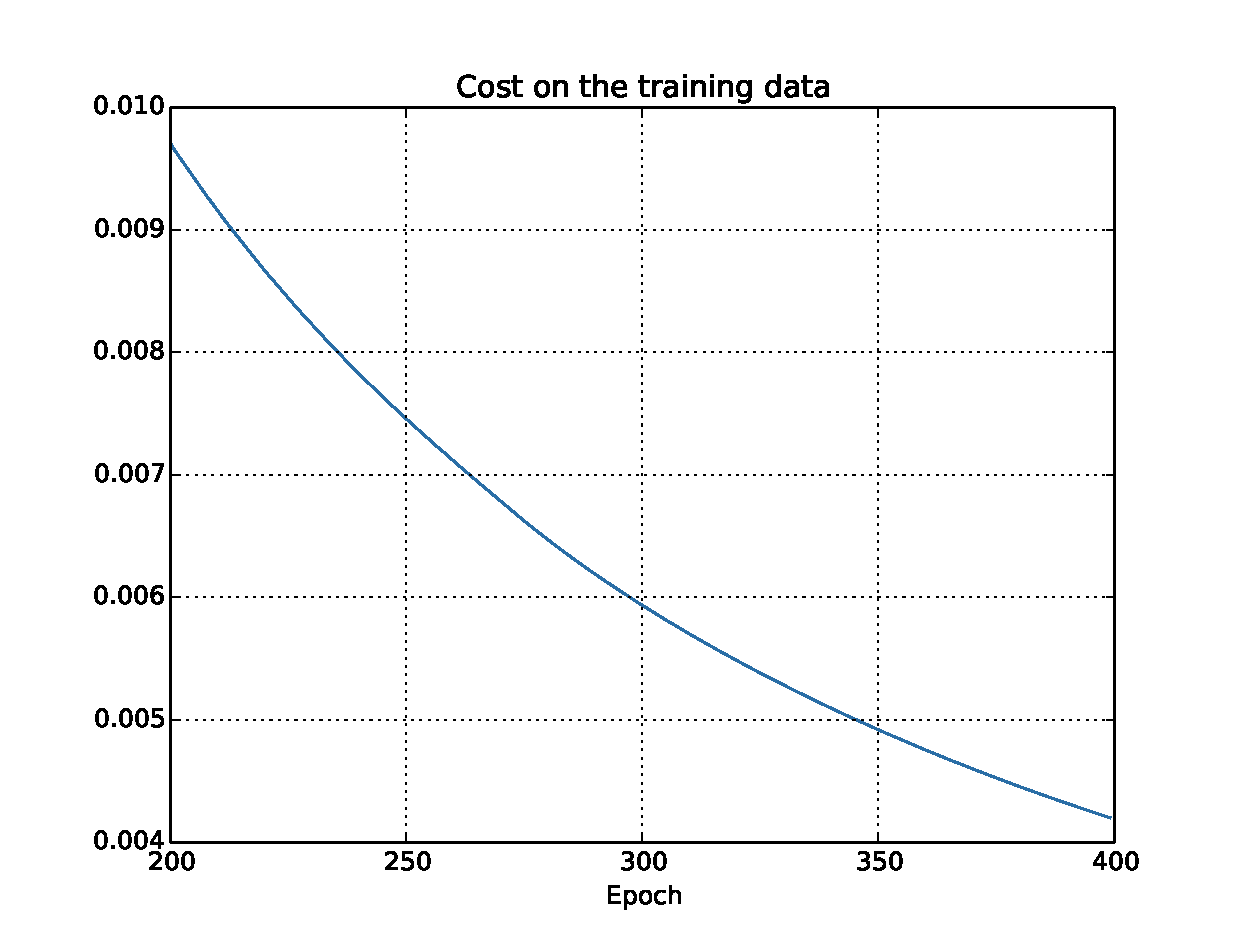
\includegraphics[width=.6\textwidth]{overfitting1}
\end{center}
  
这看起来令人振奋,因为\gls*{cost-func}有一个光滑的下降,跟我们预期一致。注意,我只是展示
了 $200$ 到 $399$ \gls*{epoch}的情况。这给出了很好的近距离理解训练后期的情况,也是出
现有趣现象的地方。

让我们看看分类准确率在测试集上的表现:
\begin{center}
  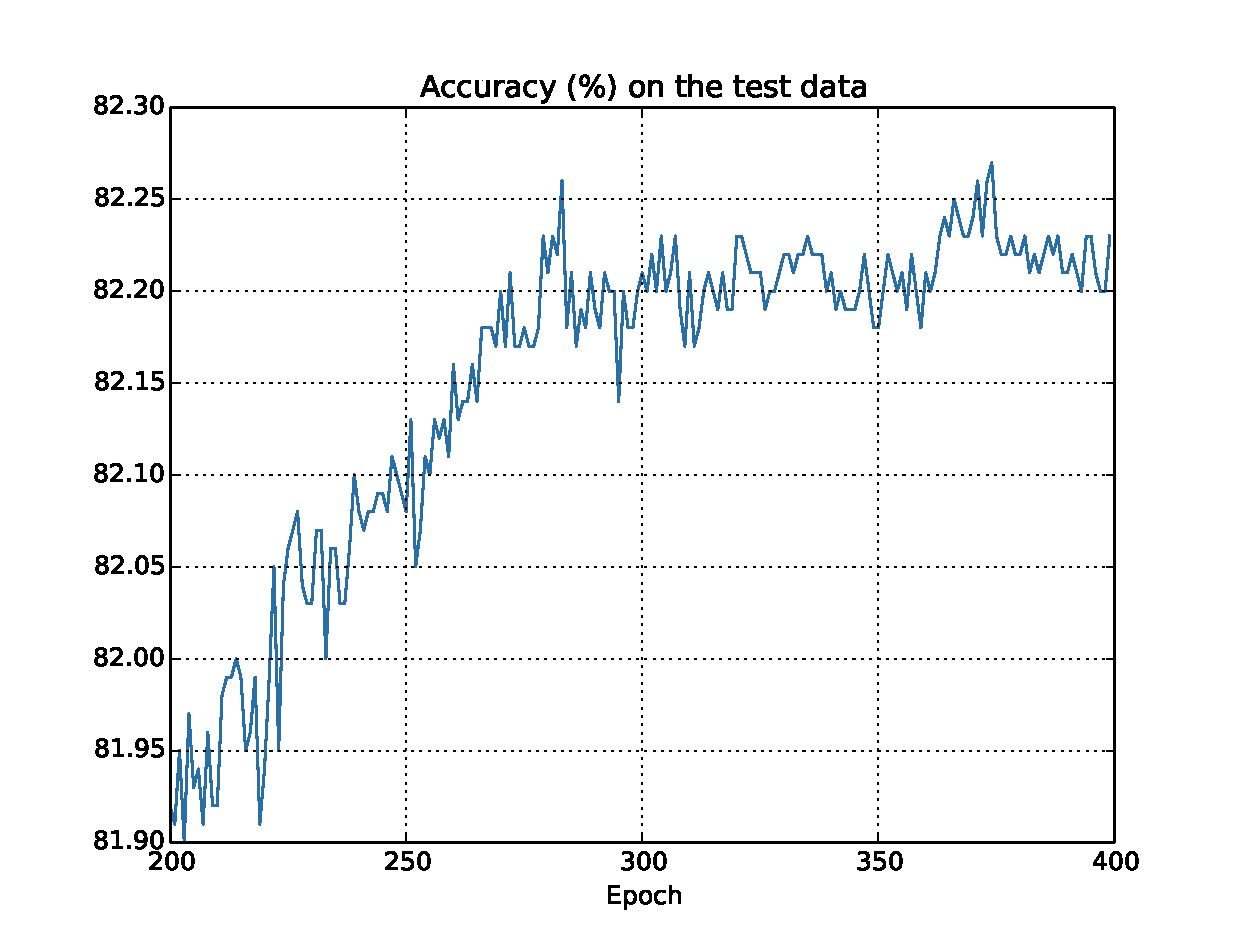
\includegraphics[width=.6\textwidth]{overfitting2}
\end{center}

这里我还是聚焦到了后面的过程。 在前 200 \gls*{epoch}(图中没有显示)中准确率提升
到了 82\%。然后学习逐渐变缓。最终,在 280 \gls*{epoch}左右分类准确率就停止了增长。
后面的\gls*{epoch},仅仅看到了在 280 \gls*{epoch}准确率周围随机的小波动。将这幅
图和前面的图进行对比,前面的图中和训练数据相关的代价持续平滑下降。如果我们只看那
个代价,会发现我们模型的表现变得“更好”。但是测试准确率展示了提升只是一种假象。
就像费米不大喜欢的那个模型一样,我们的网络在 280 \gls*{epoch}后就不再能够推广到
测试数据上。所以这不是有用的学习。我们说网络在 280 \gls*{epoch}后就%
\textbf{\gls{overfitting}}或者\textbf{\gls{overtraining}}了。

你可能想知道这里的问题是不是由于我们看的是训练数据的\textbf{代价},而对比的却是
测试数据上的\textbf{分类准确率}导致的。换言之,可能我们这里在进行苹果和橙子的对
比。如果我们比较训练数据上的代价和测试数据上的代价,会发生什么,我们是在比较类似
的度量吗?或者可能我们可以比较在两个数据集上的分类准确率啊?实际上,不管我们使用
什么度量的方式,尽管细节会变化,但本质上都是一样的。让我们来看看测试数据集上的代
价变化情况:
\begin{center}
  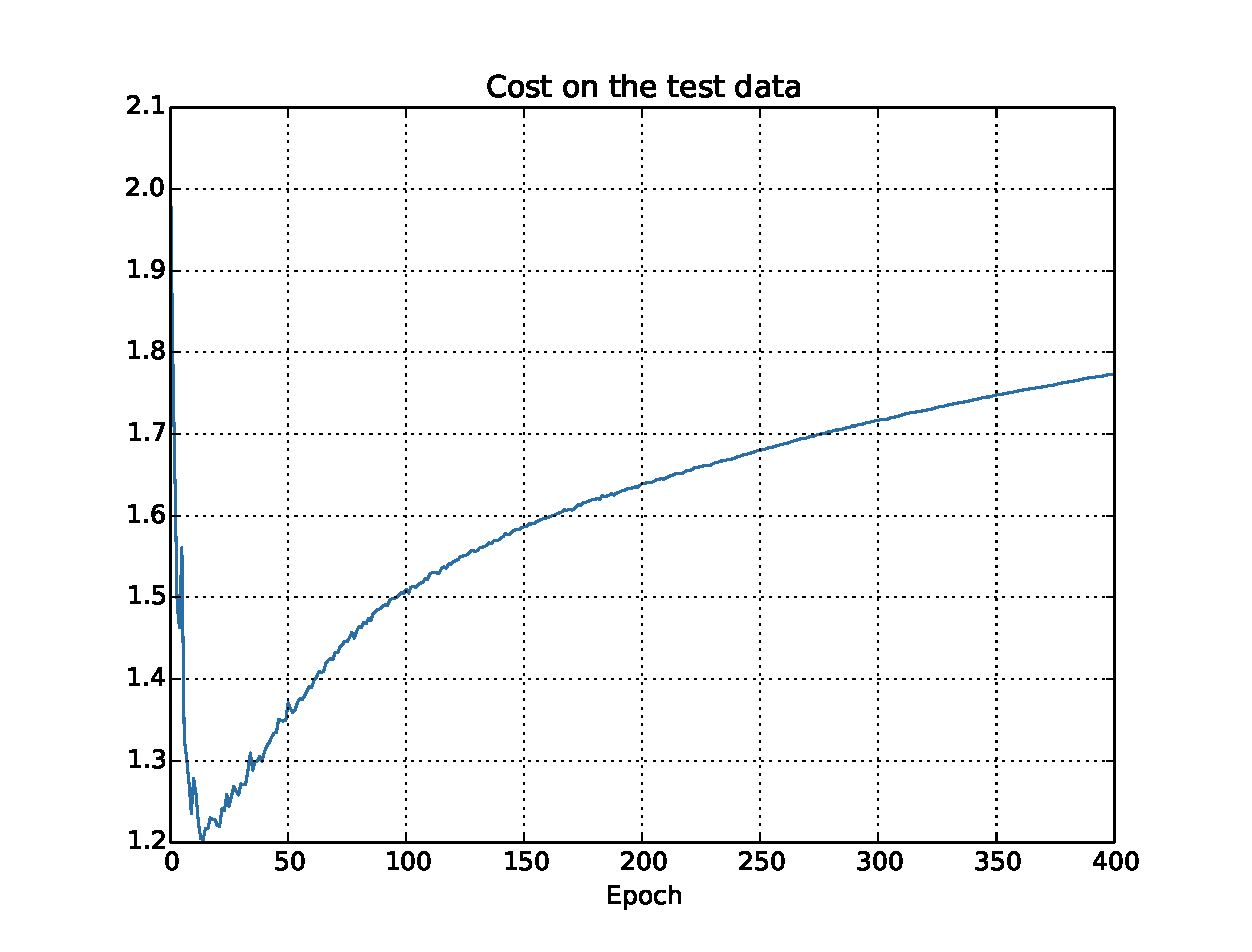
\includegraphics[width=.6\textwidth]{overfitting3}
\end{center}

我们可以看到测试集上的代价在 15 \gls*{epoch}前一直在提升,随后越来越差,尽管训练
数据集上的代价表现是越来越好的。这其实是另一种模型\gls*{overfitting}的迹象。尽管,这里带来
了关于我们应当将 15 还是 280 \gls*{epoch}当作是\gls*{overfitting}开始影响学习的时间点的困
扰。从一个实践角度,我们真的关心的是提升测试数据集上的分类准确率,而测试集合上的
代价不过是分类准确率的一个反应。所以更加合理的选择就是将 280 \gls*{epoch}看成是
\gls*{overfitting}开始影响学习的时间点。

另一个\gls*{overfitting}的迹象在训练数据上的分类准确率上也能看出来:
\begin{center}
  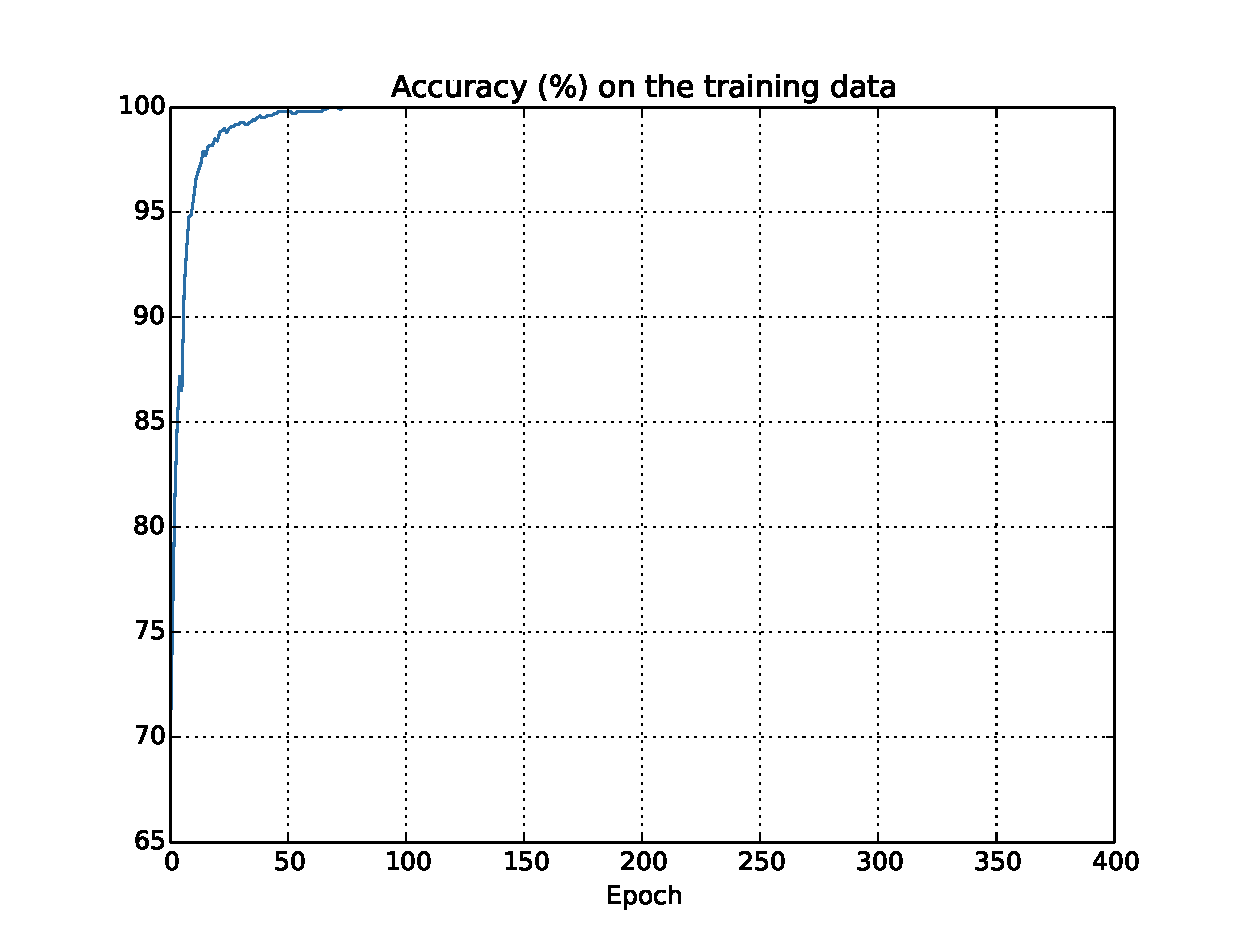
\includegraphics[width=.6\textwidth]{overfitting4}
\end{center}

准确率一直在提升接近 100\%。也就是说,我们的网络能够正确地对所有 $1000$ 幅图像进
行分类!而在同时,我们的测试准确率仅仅能够达到 82.27\%。所以我们的网络实际上在学
习训练数据集的特例,而不是能够一般地进行识别。我们的网络几乎是在单纯记忆训练集合,
而没有对数字本质进行理解能够泛化到测试数据集上。

\gls*{overfitting}是神经网络的一个主要问题。这在现代网络中特别正常,因为网络\gls*{weight}
和\gls*{bias}数量巨大。为了高效地训练,我们需要一种检测\gls*{overfitting}是不是发生的技术,
这样我们不会过度训练。并且我们也想要找到一些技术来降低\gls*{overfitting}的影响。

检测\gls*{overfitting}的明显方法是使用上面的方法~——~跟踪测试数据集合上的准确率随训练变化情
况。如果我们看到测试数据上的准确率不再提升,那么我们就停止训练。当然,严格地说,
这其实并非是\gls*{overfitting}的一个必要现象,因为测试集和训练集上的准确率可能会同时停止提
升。当然,采用这样的策略是可以阻止\gls*{overfitting}的。

实际上,我们会使用这种策略的变化形式来试验。记得之前我们载入 MNIST 数据时用了三
个数据集:

\begin{lstlisting}[language=Python]
>>> import mnist_loader
>>> training_data, validation_data, test_data = \
... mnist_loader.load_data_wrapper()
\end{lstlisting}

到现在我们一直在使用 \lstinline!training_data! 和 \lstinline!test_data!,没有用
过 \lstinline!validation_data!。\lstinline!validation_data! 中包含了 $10,000$ 幅
数字图像,这些图像和 MNIST 训练数据集中的 $50,000$ 幅图像以及测试数据集中的
$10,000$ 幅都不相同。我们会使用 \lstinline!validation_data! 而不是
\lstinline!test_data! 来防止\gls*{overfitting}。我们会为 \lstinline!test_data! 使用和上面
提到的相同的策略。我们在每个\gls*{epoch}的最后都计算在 \lstinline!validation_data!
上的分类准确率。一旦分类准确率已经饱和,就停止训练。这个策略被称为\textbf{提前停
  止}。当然,实际应用中,我们不会立即知道什么时候准确率会饱和。
相反,我们会一直训练直到我们确信准确率已经饱和\footnote{这里需要一些判定标准来确
  定什么时候停止。在我前面的图中,将 280 \gls*{epoch}看成是饱和的地方。可能这有点太
  悲观了。因为神经网络有时候会训练过程中处在一个稳定期,然后又开始提升。如果在
  400 \gls*{epoch}后,性能又开始提升(也许只是一些少量提升),那我也不会诧异。所以,
  对提前停止采取更多或更少激进的策略也是可以的。}。

\label{validation_explanation}
为何要使用 \lstinline!validation_data! 来替代 \lstinline!test_data! 防止\gls*{overfitting}
问题?实际上,这是一个更为一般的策略的一部分,这个一般的策略就是使
用 \lstinline!validation_data! 来衡量不同的超参数(如\gls*{epoch},\gls*{learning-rate},
最好的网络架构等等)的选择的效果。我们使用这样方法来找到超参数的合适值。因此,尽
管到现在我并没有提及这点,但其实本书前面已经稍微介绍了一些超参数选择的方法。(更多内容在%
\hyperref[sec:how_to_choose_a_neural_network's_hyper-parameters]{本章后面}讨论)

当然,这仍然没有回答为什么我们用 \lstinline!validation_data! 而不是
\lstinline!test_data! 来防止\gls*{overfitting}的问题。实际上,有一个更加一般的问题,就是为
何用 \lstinline!validation_data! 取代 \lstinline!test_data! 来设置更好的超参数?
为了理解这点,想想当设置超参数时,我们想要尝试许多不同的超参数选择。如果我们设置
超参数是基于 \lstinline!test_data! 的话,可能最终我们就会得到\gls*{overfitting}于
\lstinline!test_data!  的超参数。也就是说,我们可能会找到那些符合
\lstinline!test_data! 特点的超参数,但是网络的性能并不能够泛化到其他数据集合上。
我们借助 \lstinline!validation_data! 来克服这个问题。然后一旦获得了想要的超参数,
最终我们就使用 \lstinline!test_data! 进行准确率测量。这给了我们在
\lstinline!test_data! 上的结果是一个网络泛化能力真正的度量方式的信心。换言之,你
可以将验证集看成是一种特殊的训练数据集能够帮助我们学习好的超参数。这种寻找好的超
参数的方法有时候被称为\textbf{hold out}方法,因为 \lstinline!validation_data! 是从
\lstinline!traning_data! 训练集中留出或者“拿出”的一部分。

在实际应用中,甚至在衡量了 \lstinline!test_data! 的性能后,我们可能也会改变想法并
去尝试另外的方法~——~也许是一种不同的网络架构~——~这将会引入寻找新的超参数的过程。
如果我们这样做,难道不会产生\gls*{overfitting}于 \lstinline!test_data! 的困境么?我们是不是
需要一种数据集的潜在无限回归,这样才能够确信模型能够泛化?去除这样的疑惑其实是一
个深刻而困难的问题。但是对我们实际应用的目标,我们不会担心太多。相反,我们会继续
采用基
于 \lstinline!training_data!,\lstinline!validation_data!,和
\lstinline!test_data! 的基本 Hold-Out 方法。

我们已经研究了只使用 $1,000$ 幅训练图像时的\gls*{overfitting}问题。那么如果我们使用所有的
50,000 幅图像的训练数据会发生什么?我们会保留所有其它的参数都一样($30$ 个隐藏元,
  \gls*{learning-rate} $0.5$,\gls*{mini-batch}规模为 $10$),但是\gls*{epoch}为 30 次。下图
展示了分类准确率在训练和测试集上的变化情况。注意我们使用的测试数据,而不是验证集
合,为了让结果看起来和前面的图更方便比较。
\begin{center}
  \includegraphics[width=.6\textwidth]{code_samples/fig/overfitting_full}
\end{center}

如你所见,测试集和训练集上的准确率相比我们使用 $1,000$ 个训练数据时相差更小。特
别地,在训练数据上的最佳的分类准确率 97.86\% 只比测试集上的 95.33\% 准确率高了
1.53\%。而之前的例子中,这个差距是 17.73\%!\gls*{overfitting}仍然发生了,但是已经减轻了不少。
我们的网络从训练数据上更好地泛化到了测试数据上。一般来说,最好的降低\gls*{overfitting}的方式
之一就是增加训练样本的量。有了足够的训练数据,就算是一个规模非常大的网络也不大容
易\gls*{overfitting}。不幸的是,训练数据其实是很难或者很昂贵的资源,所以这不是一种太切实际的
选择。

\subsection{正则化}

增加训练样本的数量是一种减轻\gls*{overfitting}的方法。还有其他的方法能够减轻\gls*{overfitting}的程度
吗?一种可行的方式就是降低网络的规模。然而,大的网络拥有一种比小网络更强的潜力,
所以这里存在一种应用冗余性的选项。

幸运的是,还有其他的技术能够缓解\gls*{overfitting},即使我们只有一个固定的网络和固定的训练集
合。这种技术就是\textbf{\gls{regularization}}。本节,我会给出一种最为常用的\gls*{regularization}
手段~——~有时候被称为\textbf{\gls{weight-decay}}或者 \textbf{L2 \gls*{regularization}}。L2 \gls*{regularization}的想法是增加一个额外的
项到\gls*{cost-func}上,这个项叫做\textbf{\gls{regularization-term}}。下面是\gls*{regularization}的交叉熵:
\begin{equation}
  C = -\frac{1}{n} \sum_{xj} \left[ y_j \ln a^L_j+(1-y_j) \ln
  (1-a^L_j)\right] + \frac{\lambda}{2n} \sum_w w^2
\label{eq:85}\tag{85}
\end{equation}

其中第一个项就是常规的交叉熵的表达式。第二个现在加入的就是所有\gls*{weight}的平方的和。然
后使用一个因子 $\lambda / 2n$ 进行量化调整,其中 $\lambda > 0$ 可以称为\textbf{规
  范化参数},而 $n$ 就是训练集合的大小。我们会在后面讨论
$\lambda$ 的选择策略。需要注意的是,\gls*{regularization}项里面并\textbf{不}包含\gls*{bias}。这点我们后
面也会再讲述。

当然,对其他的\gls*{cost-func}也可以进行\gls*{regularization},例如二次\gls*{cost-func}。类似的\gls*{regularization}的形式如下:
\begin{equation}
  C = \frac{1}{2n} \sum_x \|y-a^L\|^2 + \frac{\lambda}{2n} \sum_w w^2
  \label{eq:86}\tag{86}
\end{equation}

两者都可以写成这样:
\begin{equation}
  C = C_0 + \frac{\lambda}{2n} \sum_w w^2
  \label{eq:87}\tag{87}
\end{equation}
其中 $C_0$ 是原始的\gls*{cost-func}。

直觉地看,\gls*{regularization}的效果是让网络倾向于学习小一点的\gls*{weight},其他的东西都一样的。
大的\gls*{weight}只有能够给出\gls*{cost-func}第一项足够的提升时才被允许。换言之,\gls*{regularization}可以当做一种寻找
小的\gls*{weight}和最小化原始的\gls*{cost-func}之间的折中。这两部分之间相对的重要性就由 $\lambda$
的值来控制了:$\lambda$ 越小,就偏向于最小化原始\gls*{cost-func},反之,倾向于小的\gls*{weight}。

现在,对于这样的折中为何能够减轻\gls*{overfitting}还不是很清楚!但是,实际表现表明了这点。我
们会在下一节来回答这个问题。但现在,我们来看看一个\gls*{regularization}的确减轻\gls*{overfitting}的例子。

为了构造这个例子,我们首先需要弄清楚如何将\gls*{sgd}算法应用在一个\gls*{regularization}的神经
网络上。特别地,我们需要知道如何计算对网络中所有\gls*{weight}和\gls*{bias}的偏导数 $\partial
C/\partial w$ 和 $\partial C/\partial b$。对方程~\eqref{eq:87} 进行求偏导数得:
\begin{align}
  \frac{\partial C}{\partial w} & = \frac{\partial C_0}{\partial w} +
                                  \frac{\lambda}{n} w \label{eq:88}\tag{88} \\
  \frac{\partial C}{\partial b} & = \frac{\partial C_0}{\partial b} \label{eq:89}\tag{89}
\end{align}

$\partial C_0/\partial w$ 和 $\partial C_0/\partial b$ 可以通过\gls*{bp}进行计算,
正如\hyperref[ch:HowTheBackpropagationAlgorithmWorks]{上一章}中描述的那样。所以
我们看到其实计算\gls*{regularization}的\gls*{cost-func}的梯度是很简单的:仅仅需要\gls*{bp},然后加上
$\frac{\lambda}{n} w$ 得到所有\gls*{weight}的偏导数。而\gls*{bias}的偏导数就不要变化,所以\gls*{bias}的
梯度下降学习规则不会发生变化:
\begin{equation}
  b \rightarrow b -\eta \frac{\partial C_0}{\partial b}
  \label{eq:90}\tag{90}
\end{equation}

\gls*{weight}的学习规则就变成:
\begin{align}
  w & \rightarrow w-\eta \frac{\partial C_0}{\partial
      w}-\frac{\eta \lambda}{n} w \label{eq:91}\tag{91}\\
    & = \left(1-\frac{\eta \lambda}{n}\right) w -\eta \frac{\partial
      C_0}{\partial w} \label{eq:92}\tag{92}
\end{align}

这正和通常的梯度下降学习规则相同,除了通过一个因子 $1-\frac{\eta\lambda}{n}$ 重
新调整了\gls*{weight} $w$。这种调整有时被称为\textbf{\gls*{weight}衰减},因为它使得\gls*{weight}变小。粗看,
这样会导致\gls*{weight}会不断下降到 $0$。但是实际不是这样的,因为如果在原始\gls*{cost-func}中造成
下降的话其他的项可能会让\gls*{weight}增加。

好的,这就是梯度下降工作的原理。那么\gls*{sgd}呢?正如在没有\gls*{regularization}的随机梯度下
降中,我们可以通过平均 $m$ 个训练样本的\gls*{mini-batch}来估计 $\partial C_0/\partial
w$。因此,为了\gls*{sgd}的\gls*{regularization}学习规则就变成(参考方程~\eqref{eq:20})
\begin{equation}
  w \rightarrow \left(1-\frac{\eta \lambda}{n}\right) w -\frac{\eta}{m}
  \sum_x \frac{\partial C_x}{\partial w}
  \label{eq:93}\tag{93}
\end{equation}
其中后面一项是在训练样本的\gls*{mini-batch} $x$ 上进行的,而 $C_x$ 是对每个训练样本的(无规
  范化的)代价。这其实和之前通常的\gls*{sgd}的规则是一样的,除了有一个\gls*{weight}下降
的因子 $1-\frac{\eta \lambda}{n}$。最后,为了完整,我给出\gls*{bias}的\gls*{regularization}的学习规则。
这当然是和我们之前的非\gls*{regularization}的情形一致了(参考公式~\eqref{eq:21}),
\begin{equation}
  b \rightarrow b - \frac{\eta}{m} \sum_x \frac{\partial C_x}{\partial b}
  \label{eq:94}\tag{94}
\end{equation}
这里求和也是在训练样本的\gls*{mini-batch} $x$ 上进行的。

让我们看看\gls*{regularization}给网络带来的性能提升吧。这里还会使用有 $30$ 个隐藏神经元、\gls*{mini-batch}
大小为 $10$,\gls*{learning-rate}为 $0.5$,使用交叉熵的神经网络。然而,这次我们会使用规
范化参数为 $\lambda = 0.1$。注意在代码中,我们使用的变量名字为 \lstinline!lmbda!,
这是因为在 Python 中 \lstinline!lambda! 是关键字,有着不相关的含义。我也会再次使
用 \lstinline!test_data!,而不是 \lstinline!validation_data!。不过严格地讲,我们
应当使用 \lstinline!validation_data! 的,因为前面已经讲过了。这里我这样做,是因
为这会让结果和非\gls*{regularization}的结果对比起来效果更加直接。你可以轻松地调整为
\lstinline!validation_data!,你会发现有相似的结果。

\begin{lstlisting}[language=Python]
>>> import mnist_loader
>>> training_data, validation_data, test_data = \
... mnist_loader.load_data_wrapper()
>>> import network2
>>> net = network2.Network([784, 30, 10], cost=network2.CrossEntropyCost)
>>> net.large_weight_initializer()
>>> net.SGD(training_data[:1000], 400, 10, 0.5,
... evaluation_data=test_data, lmbda = 0.1,
... monitor_evaluation_cost=True, monitor_evaluation_accuracy=True,
... monitor_training_cost=True, monitor_training_accuracy=True)
\end{lstlisting}

训练集上的\gls*{cost-func}持续下降,和前面无\gls*{regularization}的情况一样的规律\footnote{这个以及下一
  个图像由程序
  \href{https://github.com/mnielsen/neural-networks-and-deep-learning/blob/master/fig/overfitting.py}{overfitting.py}
  生成。}:
\begin{center}
  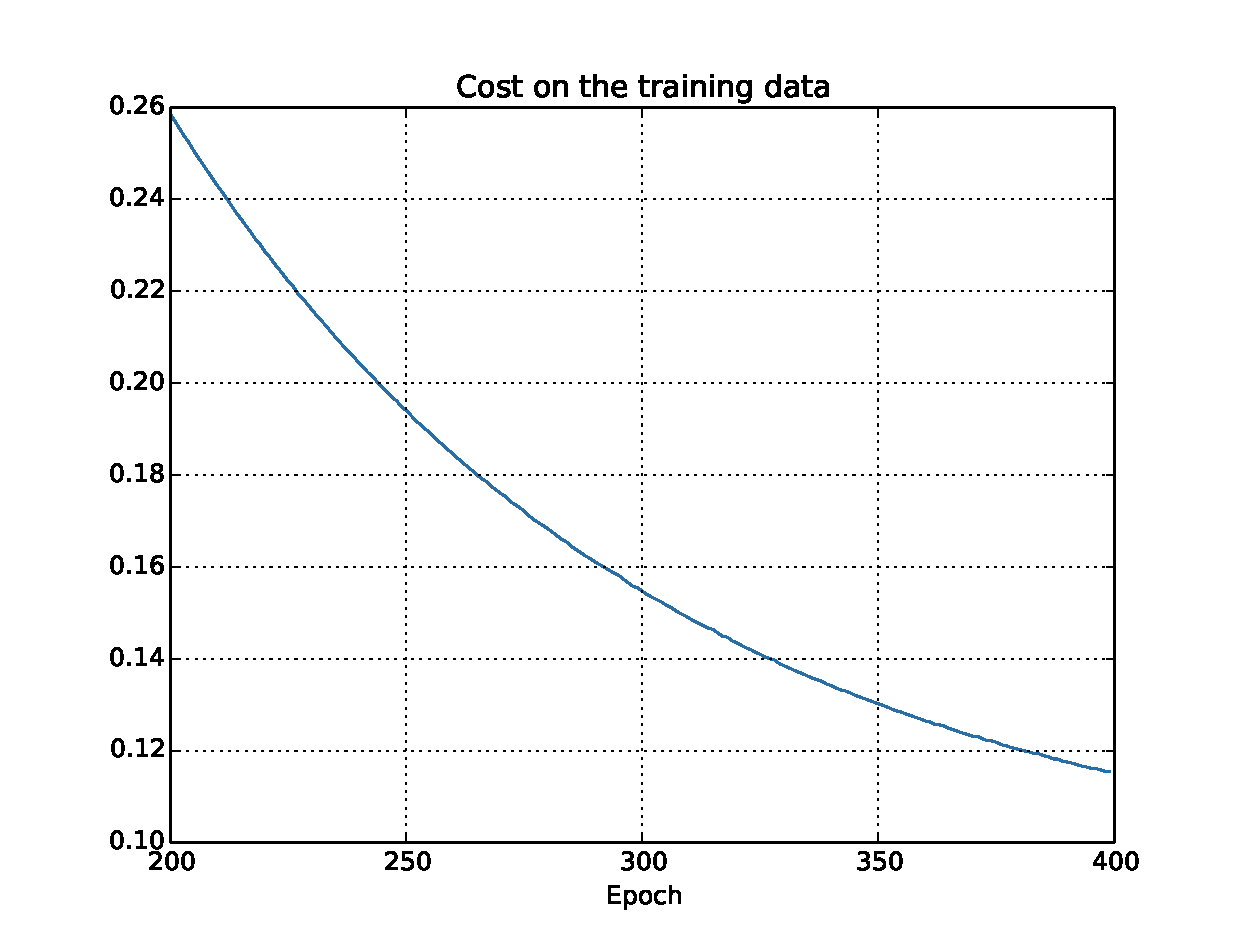
\includegraphics[width=.6\textwidth]{regularized1}
\end{center}

但是这次测试集上的准确率在整个 400 \gls*{epoch}内持续增加:
\begin{center}
  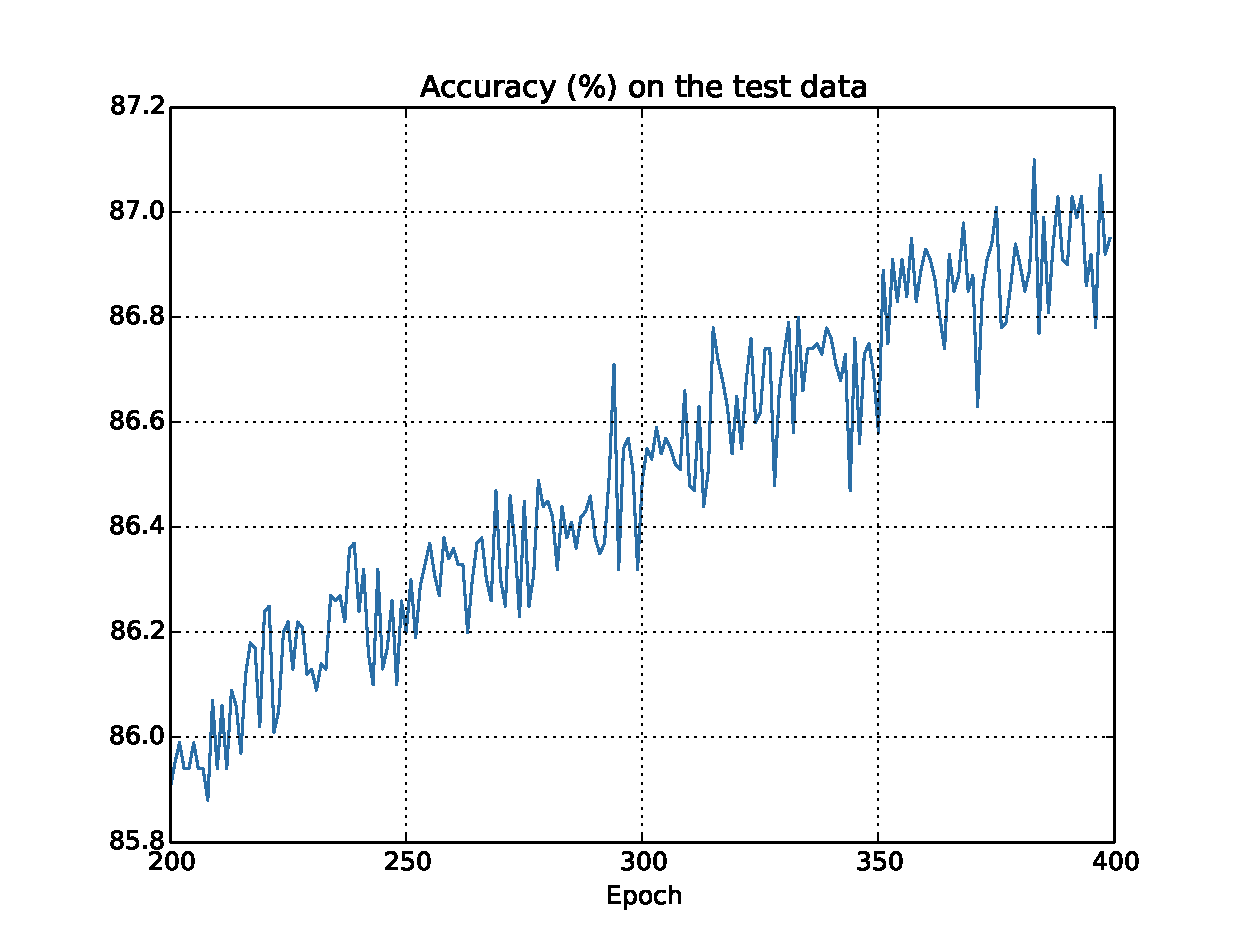
\includegraphics[width=.6\textwidth]{regularized2}
\end{center}

显然,\gls*{regularization}的使用能够解决\gls*{overfitting}的问题。而且,准确率相当高了,最高处达到了
87.1\%,相较于之前的 82.27\%。因此,我们几乎可以确信在 400 \gls*{epoch}之后持续训
练会有更加好的结果。看起来,经实践检验,\gls*{regularization}让网络具有更好的泛化能力,显著地减
轻了\gls*{overfitting}的影响。

如果我们摆脱人为的仅用 1,000 个训练图像的环境,转而用所有 50,000 图像的训练集,
会发生什么?当然,我们之前已经看到\gls*{overfitting}在大规模的数据上其实不是那么明显了。那规
范化能不能起到相应的作用呢?保持超参数和之前一样,30 \gls*{epoch}, \gls*{learning-rate}为 0.5,
\gls*{mini-batch}大小为 10。不过我们这里需要改变\gls*{regularization}参数。原因在于训练数据的大小已
经从 $n=1,000$ 改成了 $n=50,000$,这个会改变\gls*{weight}衰减因子
$1-\frac{\eta\lambda}{n}$。如果我们持续使用 $\lambda = 0.1$ 就会产生很小的\gls*{weight}衰
减,因此就将\gls*{regularization}的效果降低很多。我们通过修改为 $\lambda = 5.0$ 来补偿这种下降。

好了,来训练网络,重新初始化\gls*{weight}:

\begin{lstlisting}[language=Python]
>>> net.large_weight_initializer()
>>> net.SGD(training_data, 30, 10, 0.5,
... evaluation_data=test_data, lmbda = 5.0,
... monitor_evaluation_accuracy=True, monitor_training_accuracy=True)
\end{lstlisting}

我们得到:
\begin{center}
  \includegraphics[width=.6\textwidth]{code_samples/fig/regularized_full}
\end{center}

这个结果很不错。第一,我们在测试集上的分类准确率在使用\gls*{regularization}后有了提升,从
95.49\% 到 96.49\%。这是个很大的进步。第二,我们可以看到在训练数据和测试数据上的
结果之间的差距也更小了。这仍然是一个大的差距,不过我们已经显著得到了本质上的降低
\gls*{overfitting}的进步。

最后,我们看看在使用 100 个隐藏神经元和\gls*{regularization}参数为 $\lambda = 5.0$ 相应的测试分
类准确率。我不会给出详细分析,纯粹为了好玩,来看看我们使用一些技巧(交叉熵函数和
  L2 \gls*{regularization})能够达到多高的准确率。

\begin{lstlisting}[language=Python]
>>> net = network2.Network([784, 100, 10], cost=network2.CrossEntropyCost)
>>> net.large_weight_initializer()
>>> net.SGD(training_data, 30, 10, 0.5, lmbda=5.0,
... evaluation_data=validation_data,
... monitor_evaluation_accuracy=True)
\end{lstlisting}

最终在验证集上的准确率达到了 97.92\%。这是比 30 个隐藏元的较大飞跃。
\label{chap3_98_04_percent}实际上,稍微改变一点,60 \gls*{epoch}
$\eta=0.1$ 和$\lambda = 5.0$。我们就突破了 98\%,达到了98.04\% 的分类准确
率\label{98percent}。对于 152 行代码这个效果还真不错!

我已经把\gls*{regularization}描述为一种减轻\gls*{overfitting}和提高分类准确率的方法。实际上,这不是仅有的
好处。实践表明,在使用不同的(随机)\gls*{weight}初始化进行多次 MNIST 网络训练的时候,我发
现无\gls*{regularization}的网络会偶然被限制住,明显困在了\gls*{cost-func}的局部最优值处。结果就是不同的
运行会给出相差很大的结果。对比看来,\gls*{regularization}的网络能够提供更容易复制的结果。

为何会这样子?从经验上看,如果\gls*{cost-func}是无\gls*{regularization}的,那么\gls*{weight}向量的长度可能会增长,
而其他的东西都保持一样。随着时间的推移,这会导致\gls*{weight}向量变得非常大。所以会使得权
重向量卡在朝着更多还是更少的方向上变化,因为当长度很大的时候梯度下降带来的变化仅
仅会引起在那个方向发生微小的变化。我相信这个现象让我们的学习算法更难有效地探索权
重空间,最终导致很难找到\gls*{cost-func}的最优值。

\subsection{为何正则化可以帮助减轻过度拟合}

% I produce the 3 graphs in MATLAB:
%
% for simple_model:
% 	x = [0.976923076923080,1.48461538461538,1.99230769230769,2.58461538461538,2.83846153846154,3.43076923076923,3.60000000000000,3.72692307692308,4.10769230769231,4.53076923076923];
% 	y = [2.51111111111111,2.82222222222222,4.22222222222222,5,5.85555555555556,6.55555555555556,6.86666666666667,7.33333333333333,8.18888888888889,8.88888888888889];
% 	plot(x,y,'.k','MarkerSize', 20);
%		xlabel('\it x','FontSize',16,'FontWeight','bold')
%		ylabel('\it y','FontSize',16,'FontWeight','bold')
%
% for polynomial_fit:
% 	p = polyfit(x, y, 9);
% 	x1 = 0.95:0.05:4.55;
% 	y1 = polyval(p, x1);
%		figure
%		plot(x,y,'.k','MarkerSize', 20)
%		hold on
%		plot(x1,y1,'b')
%		hold off
% 
% for linear_fit:
% 	x2 = [0, 5];
% 	y2 = [0, 10];
%		figure
%		plot(x,y,'.k','MarkerSize', 20)
%		hold on
%		plot(x2,y2,'b')
%		hold off

我们已经看到了\gls*{regularization}在实践中能够减少\gls*{overfitting}了。这是令人振奋的,不过,这背后的原因
还不得而知!通常的说法是:小的\gls*{weight}在某种程度上,意味着更低的复杂性,也就对数据给出了一
种更简单却更强大解释,因此应该优先选择。这虽然很简短,不过暗藏了一些可能看
起来会令人困惑的因素。让我们将这个解释细化,认真地研究一下。现在给一个简单的数据
集,我们为其建立模型:
\begin{center}
  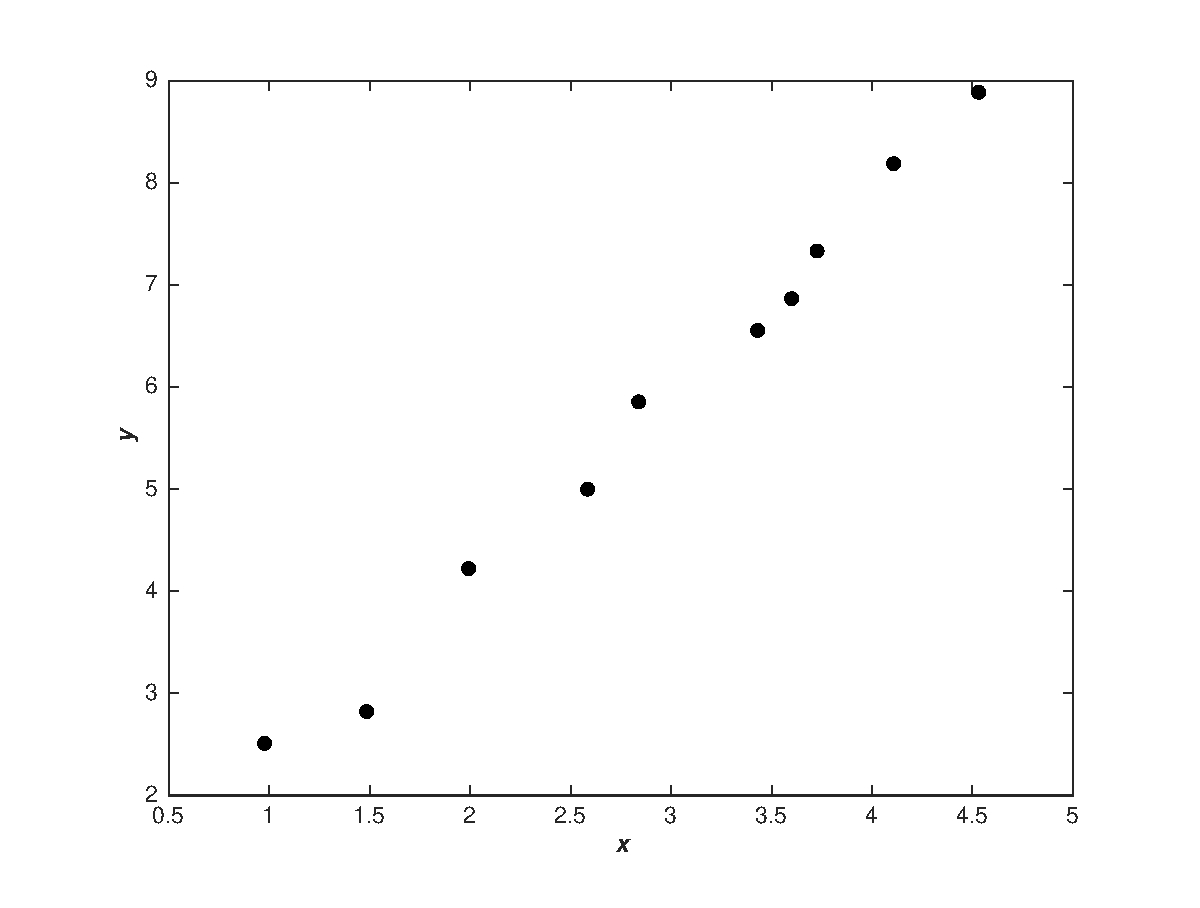
\includegraphics[width=.55\textwidth]{simple_model.eps}
\end{center}
	
这里我们其实在研究某种真实的现象,$x$ 和 $y$ 表示真实的数据。我们的目标是训练一个
模型来预测 $y$ 关于 $x$ 的函数。我们可以使用神经网络来构建这个模型,但是我们先来
个简单的:用一个多项式来拟合数据。这样做的原因其实是多项式相比神经网络能够让事情
变得更加清楚。一旦我们理解了多项式的场景,对于神经网络可以如法炮制。现在,图中有
十个点,我们就可以找到唯一的 $9$ 阶多项式 $y=a_0x^9 + a_1x^8 + ... + a_9$ 来完全
拟合数据。下面是多项式的图像\footnote{这里我不明确列出这些系数,它们很容易用一个
  例如 Numpy 的 \lstinline!polyfit! 程序就能找到。如果你对此好奇,可以从%
  \href{http://neuralnetworksanddeeplearning.com/js/polynomial_model.js}{这个图形
    的源码}中查看准确的多项式形式。其中的第 14 行的函数 \lstinline!p(x)! 生成这个
  图形。}:
\begin{center}
  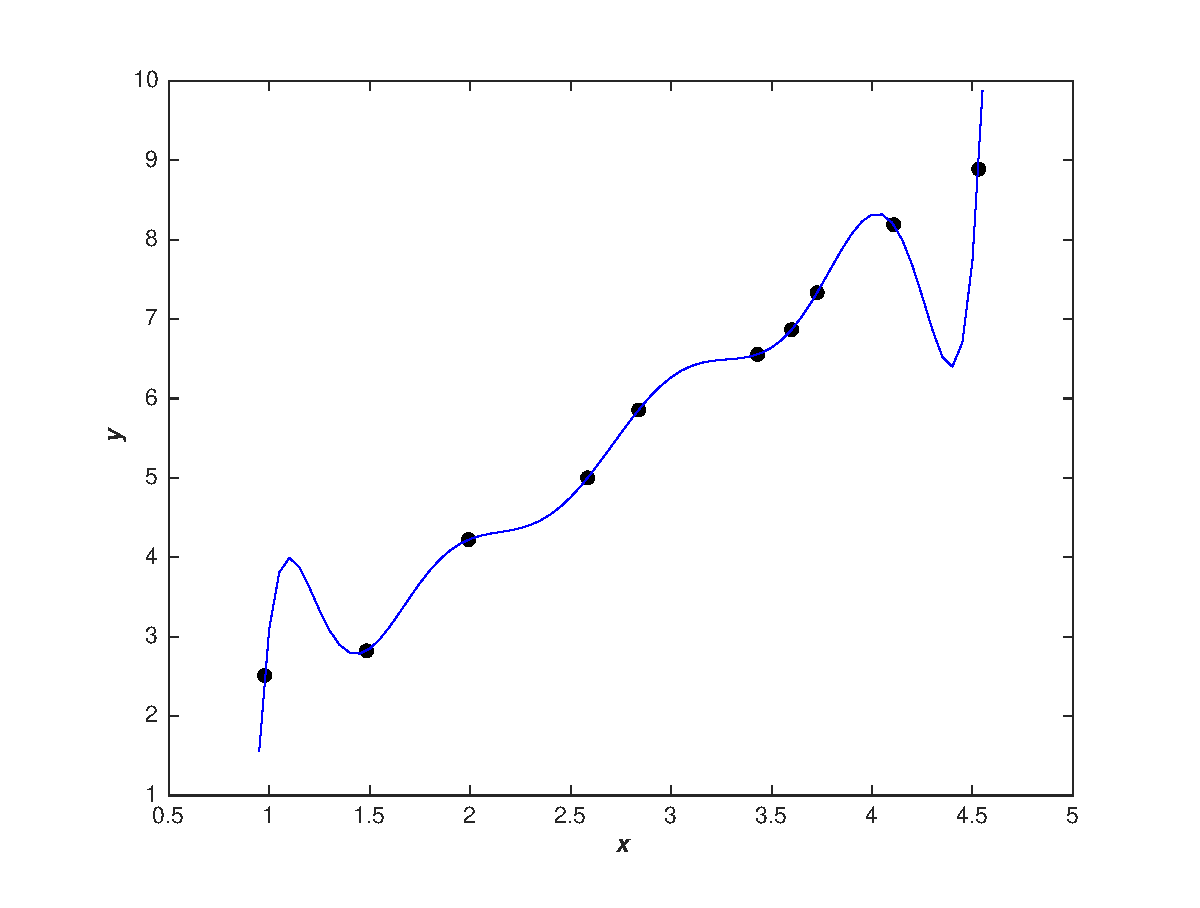
\includegraphics[width=.55\textwidth]{polynomial_fit.eps}
\end{center}

这给出了一个准确的拟合。但是我们同样也能够使用线性模型 $y=2x$ 得到一个好的拟合效
果:
\begin{center}
  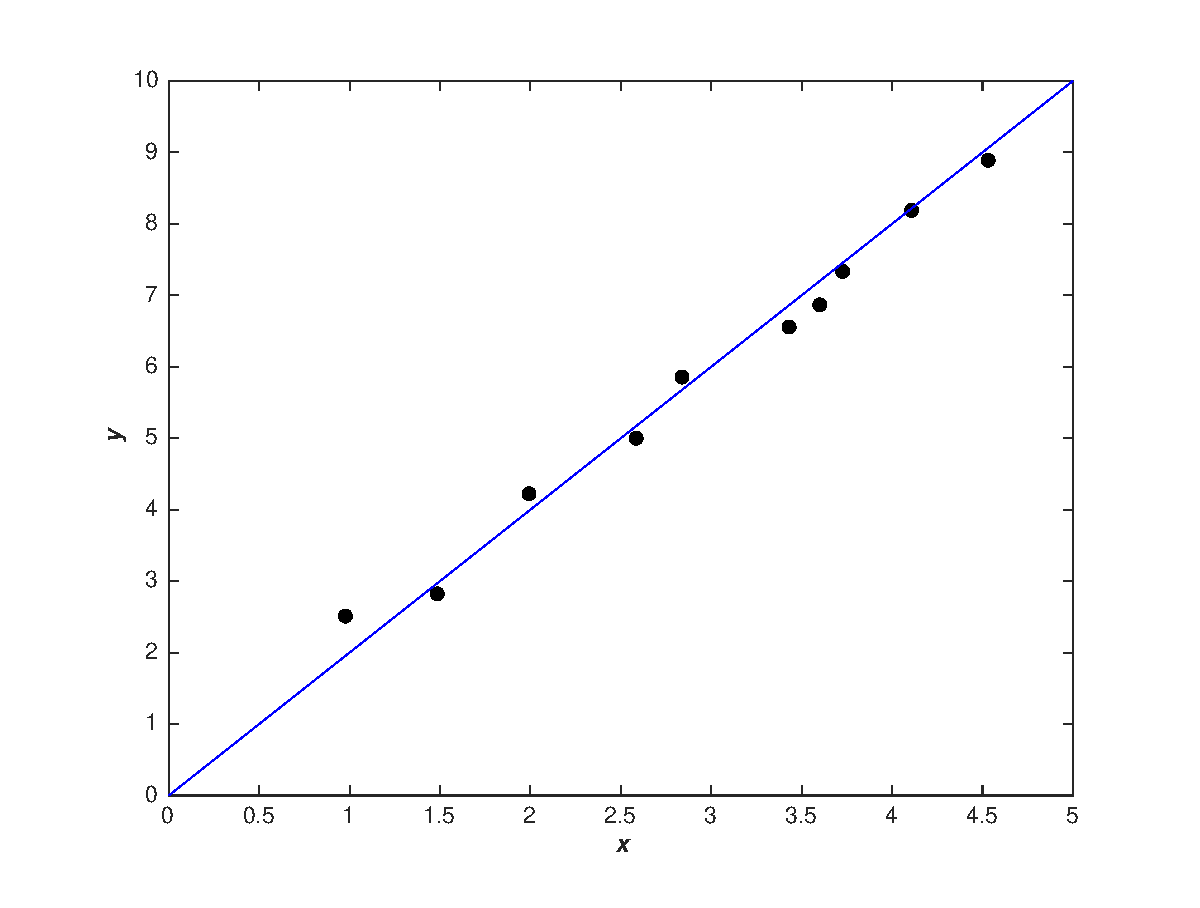
\includegraphics[width=.55\textwidth]{linear_fit.eps}
\end{center}

哪个是更好的模型?哪个更可能是真的?还有哪个模型更可能泛化到其他的拥有同样现象的
样本上?

这些都是很难回答的问题。实际上,我们如果没有更多关于真实现象背后的信息的话,并不
能确定给出上面任何一个问题的答案。但是让我们考虑两种可能的情况:(1)9 阶多项式实
际上是完全描述了真实情况的模型,最终它能够很好地泛化;(2)正确的模型是 $y=2x$,
但是存在着由于测量误差导致的额外的噪声,使得模型不能够准确拟合。

先验假设无法说出哪个是正确的(或者,如果还有其他的情况出现)。逻辑上讲,这些都可
能出现。并且这不是微不足道的差异。在给出的数据上,两个模型的表现其实是差不多的。
但是假设我们想要预测对应于某个超过了图中所有的 $x$ 的 $y$ 的值,在两个模型给出的
结果之间肯定有一个极大的差距,因为 9 阶多项式模型肯定会被 $x^9$ 主导,而线性模型
只是线性的增长。

在科学中,一种观点是我们除非不得已应该追随更简单的解释。当我们找到一个简单模型似
乎能够解释很多数据样本的时候,我们都会激动地认为发现了规律!总之,这看起来简单的
解决仅仅会是偶然出现的不大可能。我们怀疑模型必须表达出某些关于现象的内在的真理。
如上面的例子,线性模型加噪声肯定比多项式更加可能。所以如果简单性是偶然出现的话就
很令人诧异。因此我们会认为线性模型加噪声表达出了一些潜在的真理。从这个角度看,多
项式模型仅仅是学习到了局部噪声的影响效果。所以尽管多项式对于这些特定的数据点表现
得很好。模型最终会在未知数据上的泛化上出现问题,所以噪声线性模型具有更强大的预测
能力。

让我们从这个观点来看神经网络。假设神经网络大多数有很小的\gls*{weight},这最可能出现在规范
化的网络中。更小的\gls*{weight}意味着网络的行为不会因为我们随便改变了一个输入而改变太大。
这会让\gls*{regularization}网络学习局部噪声的影响更加困难。将它看做是一种让单个的证据不会影响网
络输出太多的方式。相对的,\gls*{regularization}网络学习去对整个训练集中经常出现的证据进行反应。
对比看,大\gls*{weight}的网络可能会因为输入的微小改变而产生比较大的行为改变。所以一个无规
范化的网络可以使用大的\gls*{weight}来学习包含训练数据中的噪声的大量信息的复杂模型。简言之,
\gls*{regularization}网络受限于根据训练数据中常见的模式来构造相对简单的模型,而能够抵抗训练数据
中的噪声的特性影响。我们的想法就是这可以让我们的网络对看到的现象进行真实的学习,
并能够根据已经学到的知识更好地进行泛化。

所以,倾向于更简单的解释的想法其实会让我们觉得紧张。人们有时候将这个想法称为“奥
卡姆剃刀原则”,然后就会热情地将其当成某种科学原理来应用这个法则。但是,这就不是
一个一般的科学原理。也没有任何先验的逻辑原因来说明简单的解释就比更为复杂的解释要
好。实际上,有时候更加复杂的解释其实是正确的。

让我介绍两个说明复杂正确的例子。在 1940 年代,物理学家 Marcel Schein 发布了一个发
现新粒子的声明。而他工作的公司,GE,非常欢喜,就广泛地推广这个发现。但是物理学
及 Hans Bethe 就有怀疑。Bethe 访问了 Schein,看着那些展示 Schein 的新粒子的轨迹的
盘子。但是在每个 plate 上,Bethe 都发现了某个说明数据需要被去除的问题。最
后 Schein 展示给 Bethe 一个看起来很好的 plate。Bethe 说这可能就是一个统计上的侥
幸。Schein 说,“是的,但是这个可能就是统计学,甚至是根据你自己的公式,也就
是 $1/5$ 的概率。” Bethe 说:“但我们已经看过了这 $5$ 个plate 了”。最
终,Schein 说:“但是在我的plate中,每个好的plate,每个好的场景,你使用了不同的理
论(说它们是新的粒子)进行解释,而我只有一种假设来解释所有的 plate。” Bethe 回答
说,“在你和我的解释之间的唯一差别就是你的是错的,而我所有的观点是正确的。你单一
的解释是错误的,我的多重解释所有都是正确的。”后续的工作证实了,Bethe 的想法是正
确的而 Schein 粒子不再正确\footnote{这个故事由物理学家 Richard Feynman 在一次和
历史学家 Charles Weiner 的%
  \href{https://www.aip.org/history-programs/niels-bohr-library/oral-histories/5020-4}{采访}%
  中讲述。}。

第二个例子,在 1859 年,天文学家 Urbain Le Verrier 观察到水星并没有按照牛顿万有引
力给出的轨迹进行运转。与牛顿力学只有很小的偏差,那时候一些解释就是牛顿力学需要一
些微小的改动了。在 1916 年爱因斯坦证明偏差用他的广义相对论可以解释得更好,这是一
种和牛顿重力体系相差很大的理论,基于更复杂的数学。尽管引入了更多的复杂性,现如今
爱因斯坦的解释其实是正确的,而牛顿力学即使加入一些调整,仍旧是错误的。这部分因为
我们知道爱因斯坦的理论不仅仅解释了这个问题,还有很多其他牛顿力学无法解释的问题也
能够完美解释。另外,令人印象深刻的是,爱因斯坦的理论准确地给出了一些牛顿力学没能
够预测到的显现。但是这些令人印象深刻的现象其实在先前的时代是观测不到的。如果一个
人仅仅通过简单性作为判断合理模型的基础,那么一些牛顿力学的改进理论可能会看起来更
加合理一些。

从这些故事中可以读出三点。第一,确定两种解释中哪个“更加简单”其实是一件相当微妙
的工作。第二,即使我们可以做出这样一个判断,简单性也是一个使用时需要相当小心的指
导!第三,对模型真正的测试不是简单性,而是它在新场景中对新的活动中的预测能力。

所以,我们应当时时记住这一点,\gls*{regularization}的神经网络常常能够比非\gls*{regularization}的泛化能力更强,
这只是一种实验事实(empirical fact)。所以,本书剩下的内容,我们也会频繁地使用规
范化技术。我已经在上面讲过了为何现在还没有一个人能够发展出一整套具有说服力的关于
\gls*{regularization}可以帮助网络泛化的理论解释。实际上,研究者们不断地在写自己尝试不同的\gls*{regularization}
方法,然后看看哪种表现更好,尝试理解为何不同的观点表现的更好。所以你可以将\gls*{regularization}
看做某种任意整合的技术。尽管其效果不错,但我们并没有一套完整的关于所发生情况的理
解,仅仅是一些不完备的启发式规则或者经验。

这里也有更深的问题,这个问题也是有关科学的关键问题~——~我们如何泛化。\gls*{regularization}能够给我
们一种计算上的魔力帮助神经网络更好地泛化,但是并不会带来原理上理解的指导,甚至不
会告诉我们什么样的观点才是最好的\footnote{这些问题追溯到
  \href{http://en.wikipedia.org/wiki/Problem_of_induction}{problem of
    induction},被苏格兰哲学家 David Hume 在
  \href{http://www.gutenberg.org/ebooks/9662}{"An Enquiry Concerning Human
    Understanding"} (1748)中被讨论过,这是人所共知的。归纳的问题已经在 David Wolpert 
		和 William Macready (1997)的没有免费午餐的定理下%
		(\href{http://ieeexplore.ieee.org/xpl/articleDetails.jsp?tp=&arnumber=585893}{链接})%
		被给予一个现代的机器学习的形式。}。

这实在是令人困扰,因为在日常生活中,我们人类在泛化上表现很好。给一个儿童几幅大象
的图片,他就能快速地学会认识其他的大象。当然,他们偶尔也会搞错,很可能将一只犀牛
误认为大象,但是一般说来,这个过程会相当准确。所以我们有个系统~——~人的大脑~——~拥有超
大量的自由变量。在受到仅仅少量的训练图像后,系统学会了在其他图像上的推广。某种程度
上,我们的大脑的\gls*{regularization}做得特别好!怎么做的?现在还不得而知。我期望若干年后,我们
能够发展出更加强大的技术来\gls*{regularization}神经网络,最终这些技术会让神经网络甚至在小的训练
集上也能够学到强大的泛化能力。

实际上,我们的网络已经比我们预先期望的要好一些了。拥有 100 个隐藏元的网络会有接
近 80,000 个参数。我们的训练集仅仅有 50,000 幅图像。这好像是用一个 80,000
阶的多项式来拟合 50,000 个数据点。我们的网络肯定会\gls*{overfitting}得很严重。但是,这样的
网络实际上却泛化得很好。为什么?这一点并没有很好地理解。这里有个猜想\footnote{在
  \href{http://yann.lecun.com/exdb/publis/pdf/lecun-01a.pdf}{Gradient-Based
    Learning Applied to Document Recognition} 中,作者为 Yann LeCun, Léon Bottou,
  Yoshua Bengio, 和 Patrick Haffner (1998)。}:梯度下降学习的动态有一种自\gls*{regularization}的
效应。这真是一个意料之外的巧合,但也带来了对于这种现象本质无知的不安。不过,我们
还是会在后面依照这种实践的观点来应用\gls*{regularization}技术的。神经网络也是由于这点表现才更好
一些。

现在我们回到前面留下来的一个细节:L2 \gls*{regularization}没有限制\gls*{bias},以此作为本节的结论。当然
了,对\gls*{regularization}的过程稍作调整就可以对\gls*{bias}进行规范了。实践看来,做出这样的调整并不会
对结果改变太多,所以,在某种程度上,对不对\gls*{bias}进行\gls*{regularization}其实就是一种习惯了。然而,
需要注意的是,有一个大的\gls*{bias}并不会像大的\gls*{weight}那样会让神经元对输入太过敏感。所以我
们不需要对大的\gls*{bias}所带来的学习训练数据的噪声太过担心。同时,允许大的\gls*{bias}能够让网
络更加灵活~——~因为,大的\gls*{bias}让神经元更加容易饱和,这有时候是我们所要达到的效果。所
以,我们通常不会对\gls*{bias}进行\gls*{regularization}。

\subsection{正则化的其他技术}

除了 L2 外还有很多\gls*{regularization}技术。实际上,正是由于数量众多,我这里也不会将所有的都列
举出来。在本节,我简要地给出三种减轻\gls*{overfitting}的其他的方法:L1 \gls*{regularization}、\gls*{dropout}和人为
增加训练样本。我们不会像上面介绍得那么深入。其实,目的只是想让读者熟悉这些主要的
思想,然后来体会一下\gls*{regularization}技术的多样性。\\

\textbf{L1 \gls*{regularization}:} 这个方法是在未\gls*{regularization}的\gls*{cost-func}上加上一个权
重绝对值的和:
\begin{equation}
  C = C_0 + \frac{\lambda}{n} \sum_w |w|
  \label{eq:95}\tag{95}
\end{equation}

凭直觉地看,这和 L2 \gls*{regularization}相似,惩罚大的\gls*{weight},倾向于让网络优先选择小的\gls*{weight}。当然,
L1 \gls*{regularization}和 L2 \gls*{regularization}并不相同,所以我们不应该期望从 L1 \gls*{regularization}得到完全同样的行为。
让我们来试着理解使用 L1 \gls*{regularization}训练的网络和 L2 \gls*{regularization}训练的网络所不同的行为。

首先,我们会研究一下\gls*{cost-func}的偏导数。对 \eqref{eq:95} 求导我们有:
\begin{equation}
  \frac{\partial C}{\partial w} = \frac{\partial C_0}{\partial w}
  + \frac{\lambda}{n} \, {\rm sgn}(w)
  \label{eq:96}\tag{96}
\end{equation}
其中 ${\rm sgn}(w)$ 就是 $w$ 的正负号,即 $w$ 是正数时为 $+1$,而 $w$ 为负数时为
$-1$。使用这个表达式,我们可以轻易地对\gls*{bp}进行修改从而使用基于 L1 \gls*{regularization}的随
机梯度下降进行学习。对 L1 \gls*{regularization}的网络进行更新的规则就是
\begin{equation}
  w \rightarrow w' = w-\frac{\eta \lambda}{n} \mbox{sgn}(w) - \eta \frac{\partial
  C_0}{\partial w}
  \label{eq:97}\tag{97}
\end{equation}
其中和往常一样,我们可以用一个\gls*{mini-batch}的均值来估计 $\partial C_0/\partial w$。对
比 L2 \gls*{regularization}的更新规则(参见方程~\eqref{eq:93}),
\begin{equation}
  w \rightarrow w' = w\left(1 - \frac{\eta \lambda}{n} \right)
  - \eta \frac{\partial C_0}{\partial w}
  \label{eq:98}\tag{98}
\end{equation}
在两种情形下,\gls*{regularization}的效果就是缩小\gls*{weight}。这符合我们的直觉,两种\gls*{regularization}都惩罚大的权
重。但\gls*{weight}缩小的方式不同。在 L1 \gls*{regularization}中,\gls*{weight}通过一个常量向 $0$ 进行缩小。在 L2
\gls*{regularization}中,\gls*{weight}通过一个和 $w$ 成比例的量进行缩小的。所以,当一个特定的\gls*{weight}绝对值
$|w|$ 很大时,L1 \gls*{regularization}的\gls*{weight}缩小得远比 L2 \gls*{regularization}要小得多。相反,当一个特定的权
重绝对值 $|w|$ 很小时,L1 \gls*{regularization}的\gls*{weight}缩小得要比 L2 \gls*{regularization}大得多。最终的结果就是:
L1 \gls*{regularization}倾向于聚集网络的\gls*{weight}在相对少量的高重要度连接上,而其他\gls*{weight}就会被驱使向
$0$ 接近。

我在上面的讨论中其实忽略了一个问题~——~在 $w=0$ 的时候,偏导数 $\partial
C/\partial w$ 未定义。原因在于函数 $|w|$ 在 $w=0$ 时有个“直角”,事实上,导数是
不存在的。不过也没有关系。我们下面要做的就是应用通常的(无\gls*{regularization}的)\gls*{sgd}
的规则在 $w=0$ 处。这应该不会有什么问题,凭直觉地看,\gls*{regularization}的效果就是缩小\gls*{weight},
显然,不能对一个已经是 $0$ 的\gls*{weight}进行缩小了。更准确地说,我们将会使用方
程~\eqref{eq:96} 和~\eqref{eq:97} 并约定 $\mbox{sgn}(0) = 0$。这样就给出了一种细
致又紧凑的规则来进行采用 L1 \gls*{regularization}的\gls*{sgd}学习。\\

\textbf{\gls{dropout}:} \gls*{dropout}是一种相当激进的技术。
和 L1、L2 \gls*{regularization}不同,\gls*{dropout}技术并不依赖对\gls*{cost-func}的修改。而是,在\gls*{dropout}中,我们改变
了网络本身。在介绍它为什么能工作,以及所得到的结果前,让我描述一下\gls*{dropout}基本的工作
机制。

假设我们尝试训练一个网络:
\begin{center}
  \includegraphics{tikz30}
\end{center}

特别地,假设我们有一个训练数据 $x$ 和 对应的目标输出 $y$。通常我们会通过在网络中
前向传播 $x$ ,然后进行\gls*{bp}来确定对梯度的贡献。使用\gls*{dropout}技术,这个过程就改了。
我们会从随机(临时)地删除网络中的一半的隐藏神经元开始,同时让输入层和输出层的神经元保持
不变。在此之后,我们会得到最终如下线条所示的网络。注意那些被\gls*{dropout}的神经元,即那些临时被删
除的神经元,用虚圈表示在图中:
\begin{center}
  \includegraphics{tikz31}
\end{center}

我们前向传播输入 $x$,通过修改后的网络,然后\gls*{bp}结果,同样通过这个修改后的网
络。在一个\gls*{mini-batch}的若干样本上进行这些步骤后,我们对有关的\gls*{weight}和\gls*{bias}进
行更新。然后重复这个过程,首先重置\gls*{dropout}的神经元,然后选择一个新的随机的隐藏神经元
的子集进行删除,估计对一个不同的\gls*{mini-batch}的梯度,然后更新\gls*{weight}和\gls*{bias}。

通过不断地重复,我们的网络会学到一个\gls*{weight}和\gls*{bias}的集合。当然,这些\gls*{weight}和\gls*{bias}也是在
一半的隐藏神经元被\gls*{dropout}的情形下学到的。当我们实际运行整个网络时,是指两倍的隐藏神
经元将会被激活。为了补偿这个,我们将从隐藏神经元出去的\gls*{weight}减半。

这个\gls*{dropout}过程可能看起来奇怪,像是临时安排的。为什么我们会指望这样的方法能够进行规
范化呢?为了解释所发生的事,我希望你停下来想一下标准(没有\gls*{dropout})的训练方式。
特别地,想象一下我们训练几个不同的神经网络,都使用同一个训练数据。当然,网络可能
不是从同一初始状态开始的,最终的结果也会有一些差异。出现这种情况时,我们可以使用
一些平均或者投票的方式来确定接受哪个输出。例如,如果我们训练了五个网络,其中三个
把一个数字分类成 “3”,那很可能它就是“3”。另外两个可能就犯了错误。这种平均的
方式通常是一种强大(尽管代价昂贵)的方式来减轻\gls*{overfitting}。原因在于不同的网络可能会
以不同的方式\gls*{overfitting},平均法可能会帮助我们消除那样的\gls*{overfitting}。

那么这和\gls*{dropout}有什么关系呢?启发式地看,当我们\gls*{dropout}掉不同的神经元集合时,有点像我们
在训练不同的神经网络。所以,\gls*{dropout}过程就如同大量不同网络的效果的平均那样。不同的网
络会以不同的方式\gls*{overfitting}了,所以,\gls*{dropout}过的网络的效果会减轻\gls*{overfitting}。

一个相关的启发式解释\label{dropout_explanation}在早期使用这项技术的论文中曾经给
出\footnote{\href{https://papers.nips.cc/paper/4824-imagenet-classification-with-deep-convolutional-neural-networks.pdf}{ImageNet
    Classification with Deep Convolutional Neural Networks},作者为 Alex Krizhevsky,
  Ilya Sutskever, 和 Geoffrey Hinton (2012)。}:“因为神经元不能依赖其他神经元特
定的存在,这个技术其实减少了复杂的互适应的神经元。所以,强制要学习那些在神经元的
不同随机子集中更加健壮的特征。” 换言之,如果我们将我们的神经网络看做一个进行预
测的模型的话,我们就可以将\gls*{dropout}看做是一种确保模型对于一部分证据丢失健壮的方式。这
样看来,\gls*{dropout}和 L1、L2 \gls*{regularization}也是有相似之处的,这也倾向于更小的\gls*{weight},最后让网络对
丢失个体连接的场景更加健壮。

当然,\gls*{dropout}技术的真正衡量是它已经在提升神经网络性能上应用得相当成功。原始论
文\footnote{\href{http://arxiv.org/pdf/1207.0580.pdf}{Improving neural networks
    by preventing co-adaptation of feature detectors}, 作者为 Geoffrey Hinton, Nitish
  Srivastava, Alex Krizhevsky, Ilya Sutskever, 和 Ruslan Salakhutdinov
  (2012)。 注意这篇论文讨论了许多细微之处,这些我在这个简要的介绍里敷衍地带过了。}介
绍了将其应用于很多不同任务的技术。对我们来说,特别感兴趣的是他们应用\gls*{dropout}在 MNIST
数字分类上,使用了一个和我们之前介绍的那种普通的前向神经网络。这篇论文提及到当前
最好的结果是在测试集上取得了 98.4\% 的准确率。他们使用\gls*{dropout}和 L2 \gls*{regularization}的组合将其
提高到了 98.7\%。类似重要的结果在其他不同的任务上也取得了一定的成效,包括图像和
语音识别、自然语言处理。\gls*{dropout}技术在训练大规模深度网络时尤其有用,这样的网络中过度
拟合问题经常特别突出。\\

\textbf{人为扩展训练数据:} 我们前面看到了 MNIST 分类准确率在我们使用 1,000 幅训
练图像时候下降到了 80\% 中间的准确率。这种情况并不奇怪,因为更少的训练数据意味着
我们的网络接触更少的人类手写的数字中的变化。让我们训练 30 个隐藏神经元的网络,使
用不同的训练数据集,来看看性能的变化情况。我们使用\gls*{mini-batch}大小为 $10$,%
\gls*{learning-rate}为 $\eta=0.5$,\gls*{regularization}参数是 $\lambda=5.0$,交叉熵\gls*{cost-func}。
我们在全部训练数据集合上训练 30 个\gls*{epoch},然后会随着训练数据量的下降而成比
例增加\gls*{epoch}的数量。为了确保\gls*{weight}衰减因子在训练数据集上相同,我们
会在全部训练集上使用\gls*{regularization}参数为 $\lambda = 5.0$,然后在使用更小的训练集的时候成
比例地降低$\lambda$ 值\footnote{这个以及下两个图形由程序
  \href{https://github.com/mnielsen/neural-networks-and-deep-learning/blob/master/fig/more_data.py}{\lstinline!more_data.py!}
  生成}。
\begin{center}
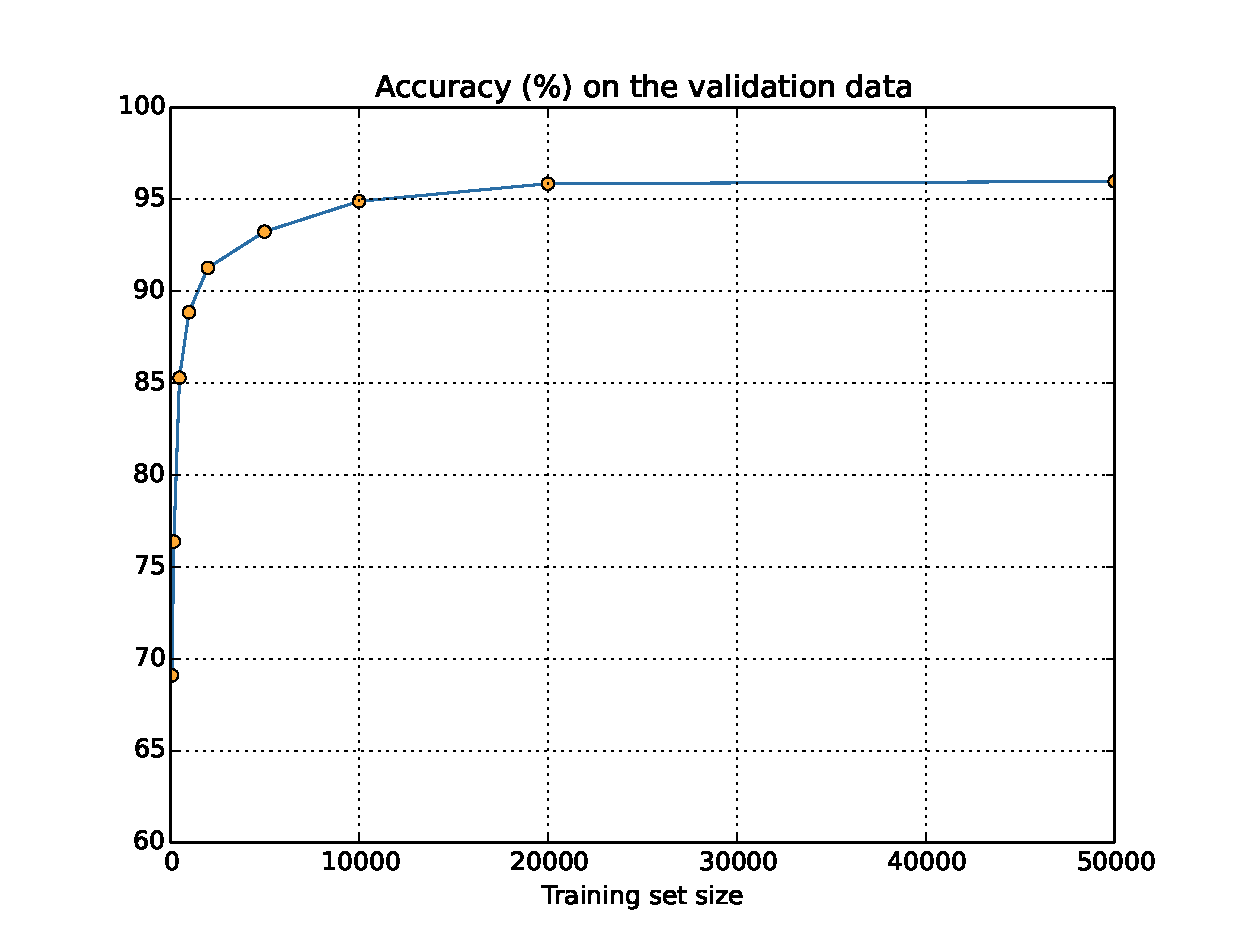
\includegraphics[width=.6\textwidth]{more_data}
\end{center}

如你所见,分类准确率在使用更多的训练数据时提升了很大。根据这个趋势的话,提升会随
着更多的数据而不断增加。当然,在训练的后期我们看到学习过程已经接近饱和状态。然而,
如果我们使用对数作为横坐标的话,可以重画此图如下:
\begin{center}
\includegraphics[width=.6\textwidth]{more_data_log}
\end{center}

这看起来到了后面结束的地方,增加仍旧明显。这表明如果我们使用大量更多的训练数据
~——~不妨设百万或者十亿级的手写样本,而不是仅仅 50,000个~——~那么,我们可能会得
到更好的性能,即使是用这样的简单网络。

获取更多的训练样本其实是很好的想法。不幸的是,这个方法代价很大,在实践中常常是很
难达到的。不过,还有一种方法能够获得类似的效果,那就是人为扩展训练数据。假设我们
使用一个 5 的 MNIST 训练图像,
\begin{center}
  \includegraphics[height=32pt]{more_data_5}
\end{center}
将其进行旋转,比如说 $15^{\circ}$:
\begin{center}
  \includegraphics[height=32pt]{more_data_rotated_5}
\end{center}

这还是会被设别为同样的数字的。但是在像素层级这和任何一幅在 MNIST 训练数据中的图
像都不相同。所以将这样的样本加入到训练数据中是很可能帮助我们的网络学会更多如何分
类数字。而且,显然我们不限于只增加这幅图像。我们可以在\textbf{所有的} MNIST训练
样本上通过\textbf{很多}小的旋转扩展训练数据,然后使用扩展后的训练数据来提升我们
网络的性能。

这个想法非常强大并且已经被广泛应用了。让我们从一篇论
文\footnote{\href{http://dx.doi.org/10.1109/ICDAR.2003.1227801}{Best Practices
    for Convolutional Neural Networks Applied to Visual Document Analysis},作者为
  Patrice Simard, Dave Steinkraus, 和 John Platt (2003)}看看一些结果,这篇论文
中,作者在 MNIST 上使用了几个这种想法的变化方式。其中一种他们考虑的网络结构其
实和我们已经使用过的类似~——~一个拥有 800 个隐藏元的前馈神经网络,使用了交叉熵代
价函数。在标准的 MNIST 训练数据上运行这个网络,得到了 98.4\% 的分类准确率。他们
不只旋转,还转换和扭曲图像来扩展训练数据。通过在这个扩展后的数据集上的训练,他们
提升到了 98.9\% 的准确率。然后还在“弹性扭曲”的数据上进行了实验,这是一种特殊的
为了模仿手部肌肉的随机抖动的图像扭曲方法。通过使用弹性扭曲扩展的数据,他们最终达
到了 99.3\% 的分类准确率。他们通过展示训练数据的所有类型的变化形式来扩展网络的经
验。

这个想法的变化形式也可以用在提升手写数字识别之外不同学习任务上的性能。一般就是通
过应用反映真实世界变化的操作来扩展训练数据。找到这些方法其实并不困难。例如,你要
构建一个神经网络来进行语音识别。我们人类甚至可以在有背景噪声的情况下识别语音。所
以你可以通过增加背景噪声来扩展你的训练数据。我们同样能够对其进行加速和减速来获得
相应的扩展数据。所以这是另外的一些扩展训练数据的方法。这些技术并不总是有用~——~例
如,其实与其在数据中加入噪声,倒不如先对数据进行噪声的清理,这样可能更加有效。当
然,记住可以进行数据的扩展,寻求应用的机会还是相当有价值的一件事。

\subsection*{练习}

\begin{itemize}
\item 正如上面讨论的那样,一种扩展 MNIST 训练数据的方式是用一些小的旋转。如果我
  们允许过大的旋转,则会出现什么状况呢?
\end{itemize}

\textbf{关于大数据和其对分类准确率的影响的题外话:} 让我们再看看神经网络准确率随
着训练集大小变化的情况:
\begin{center}
\includegraphics[width=.6\textwidth]{more_data_log}
\end{center}

假设我们使用别的机器学习技术来分类数字,而不是神经网络。例如,让我们试试使用支持
向量机(SVM),我们在%
\hyperref[ch:UsingNeuralNetsToRecognizeHandwrittenDigits]{第一章}已经简要介绍过
它。正如第一章中的情况,不要担心你熟不熟悉 SVM,我们不进行深入的讨论。我们使用
\href{http://scikit-learn.org/stable/}{scikit-learn 库}提供的 SVM 替换神经网络。
下面是 SVM 模型的性能随着训练数据集的大小变化的情况,我也画出了神经网络的结果来
方便对比\footnote{这个图形由程序
  \href{https://github.com/mnielsen/neural-networks-and-deep-learning/blob/master/fig/more_data.py}{\lstinline!more_data.py!}
  生成(和上面几个图形一样)。}:
\begin{center}
\includegraphics[width=.6\textwidth]{more_data_comparison}
\end{center}

可能第一件让你吃惊的是神经网络在每个训练规模下性能都超过了 SVM。这很好,尽管你对
细节和原理可能不太了解,因为我们只是直接从 scikit-learn 中直接调用了这个方法,而
对神经网络已经深入讲解了很多。更加微妙和有趣的现象其实是如果我们训练 SVM 使用
50,000 幅图像,那么实际上它的准确率(94.48\%)已经能够超过我们使用 5,000 幅图像
的神经网络的准确率(93.24\%)。换言之,更多的训练数据可以补偿不同的机器学习算法
的差距。

还有更加有趣的现象也出现了。假设我们试着用两种机器学习算法去解决问题,算法 A 和
算法 B。有时候出现,算法 A 在一个训练集合上超过算法 B,却在另一个训练集上弱于算
法 B。上面我们并没有看到这个情况~——~因为这要求两幅图有交叉的点~——~这里并没
有\footnote{显著的例子参见
  \href{http://dx.doi.org/10.3115/1073012.1073017}{Scaling to very very large
    corpora for natural language disambiguation},作者为 Michele Banko 和 Eric
  Brill (2001)。}。对“算法 A 是不是要比算法 B 好?”正确的反应应该是“你在使用什
么训练集合?”

在进行开发时或者在读研究论文时,这都是需要记住的事情。很多论文聚焦在寻找新的技巧
来给出标准数据集上更好的性能。“我们的超赞的技术在标准测试集 Y 上给出了百分之 X
的性能提升。”这是通常的研究声明。这样的声明通常比较有趣,不过也必须被理解为仅仅
在特定的训练数据集上的应用效果。那些给出基准数据集的人们会拥有更大的研究经费支持,
这样能够获得更好的训练数据。所以,很可能他们由于超赞的技术的性能提升其实在更大的
数据集合上就丧失了。换言之,人们标榜的提升可能就是历史的偶然。所以需要记住的特别
是在实际应用中,我们想要的是更好的算法\textbf{和}更好的训练数据。寻找更好的算法很
好,不过需要确保你在此过程中,没有放弃对更多更好的数据的追求。

\subsection*{问题}

\begin{itemize}
\item \textbf{(研究问题)} 我们的机器学习算法在非常大的数据集上如何进行?对任何
  给定的算法,其实去定义一个随着训练数据规模变化的渐近的性能是一种很自然的尝试。
  一种简单粗暴的方法就是简单地进行上面图中的趋势分析,然后将图像推进到无穷大。而
  对此想法的反驳是曲线本身会给出不同的渐近性能。你能够找到拟合某些特定类别曲线的
  理论上的验证方法吗?如果可以,比较不同的机器学习算法的渐近性能。
\end{itemize}

\textbf{总结:} 我们现在已经介绍完了\gls*{overfitting}和\gls*{regularization}。当然,我们会重回这个问题。
正如我已经提过了几次,\gls*{overfitting}是神经网络中一个重要的问题,尤其是计算机越来越强大,
我们有训练更大的网络的能力时。我们有迫切的需要来开发出强大的\gls*{regularization}技术来减轻过度
拟合,而这也是当前研究的极其活跃的领域。

\section{权重初始化}
\label{sec:weight_initialization}

创建了神经网络后,我们需要进行\gls*{weight}和\gls*{bias}的初始化。到现在,我们一直是根据在%
\hyperref[ch:UsingNeuralNetsToRecognizeHandwrittenDigits]{第一章中}介绍的那样进
行初始化。提醒你一下,之前的方式就是根据独立高斯随机变量来选择\gls*{weight}和\gls*{bias},其被归
一化为均值为 $0$,标准差 $1$。这个方法工作的还不错,但是非常\textbf{特别},所以值
得去重新探讨它,看看是否能寻找一些更好的方式来设置初始的\gls*{weight}和\gls*{bias},这也许能帮助
我们的网络学习得更快。

结果表明,我们可以比使用归一化的高斯分布做得更好。为什么?假设我们使用一个有大量
输入神经元的网络,比如说 $1,000$ 个。假设,我们已经使用归一化的高斯分布初始化了
连接第一个隐藏层的\gls*{weight}。现在我将注意力集中在这一层的连接\gls*{weight}上,忽略网络其他部分:
\begin{center}
  \includegraphics{tikz32}
\end{center}

为了简化,假设我们使用训练输入 $x$,其中一半的输入神经元值为 $1$,另一半为 $0$。
以下的论点更普遍适用,但你可以从这种特殊情况得到要点。让我们考虑隐藏神经元输入的
带权和 $z=\sum_j w_j x_j + b$。其中 $500$ 个项消去了,因为对应的输入$x_j$ 为 $0$。
所以 $z$ 是遍历总共 $501$ 个归一化的高斯随机变量的和,包含 $500$ 个\gls*{weight}项和额外
的 $1$ 个\gls*{bias}项。因此 $z$ 本身是一个均值为 $0$ 标准差为 $\sqrt{501} \approx
22.4$的高斯分布。$z$ 其实有一个非常宽的高斯分布,完全不是非常尖的形状:
\begin{center}
  \includegraphics{wide_gaussian}
\end{center}

尤其是,我们可以从这幅图中看出 $|z|$ 会变得非常的大,即 $z \gg 1$ 或者 $z \ll
-1$。如果是这样,隐藏神经元的输出 $\sigma(z)$ 就会接近 $1$ 或者 $0$。也就表示我
们的隐藏神经元会饱和。所以当出现这样的情况时,在\gls*{weight}中进行微小的调整仅仅会给隐藏
神经元的激活值带来极其微弱的改变。而这种微弱的改变也会影响网络中剩下的神经元,然
后会带来相应的\gls*{cost-func}的改变。结果就是,这些\gls*{weight}在我们进行梯度下降算法时会学习得
非常缓慢\footnote{我们在第二章详细讨论过这个问题,其中我们用%
  \hyperref[sec:the_four_fundamental_equations_behind_backpropagation]{\gls*{bp}
    的方程}来显示输入到饱和神经元的\gls*{weight}学习得缓慢。}。这其实和我们在本章前面讨论
的问题差不多,前面的情况是输出神经元在错误的值上饱和导致学习的下降。我们之前通过
\gls*{cost-func}的选择解决了前面的问题。不幸的是,尽管那种方式在输出神经元上有效,但对于
隐藏神经元的饱和却一点作用都没有。

我已经讨论了第一个隐藏层的\gls*{weight}输入。当然,类似的论证也适用于后面的隐藏层:如果后
面隐藏层的\gls*{weight}也是用归一化的高斯分布进行初始化,那么激活值将会非常接近 $0$ 或者
$1$,学习速度也会相当缓慢。

还有可以帮助我们进行更好地初始化,能够避免这种类型的饱和,最终避免学习速度的下降?
假设我们有一个有 $n_{\rm in}$ 个输入\gls*{weight}的神经元。我们会使用均值为 $0$ 标准差为
$1/\sqrt{n_{\rm in}}$ 的高斯随机分布初始化这些\gls*{weight}。也就是说,我们会向下挤压高斯
分布,让我们的神经元更不可能饱和。我们会继续使用均值为 $0$ 标准差为 $1$ 的高斯分
布来对\gls*{bias}进行初始化,后面会告诉你原因。有了这些设定,带权和 $z = \sum_j w_j x_j
+ b$ 仍然是一个均值为 $0$, 不过有尖锐峰值的高斯分布。假设,我们有 $500$ 个值为
$0$ 的输入和 $500$ 个值为 $1$ 的输入。那么很容易证明 $z$ 是服从均值为 $0$ 标准差
为$\sqrt{3/2} = 1.22\ldots$ 的高斯分布。这要比以前有更尖锐的峰值,尖锐到为了用下
图更直观地比较,我不得不对对纵坐标进行压缩:
\begin{center}
  \includegraphics{narrow_gaussian}
\end{center}

这样的一个神经元更不可能饱和,因此也不大可能遇到学习速度下降的问题。

\subsection*{练习}

\begin{itemize}
\item 验证 $z = \sum_j w_j x_j + b$ 标准差为 $\sqrt{3/2}$。下面两点可能会有帮助:
  (a)独立随机变量和的方差,是每个独立随机变量方差的和;(b)方差是标准差的平方。
\end{itemize}

我在上面提到,我们会继续使用之前的方式对\gls*{bias}进行初始化,就是使用均值为 $0$ 标准差为
$1$ 的高斯分布来对\gls*{bias}进行初始化。这其实是可行的,因为这样并不会让我们的神经网络
更容易饱和。实际上,考虑到已经避免了饱和的问题,如何初始化\gls*{bias}影响不大。有些人
将所有的\gls*{bias}初始化为 $0$,依赖梯度下降来学习合适的\gls*{bias}。但是因为差别不是很大,我
们后面还会按照前面的方式来进行初始化。

让我们在 MNIST 数字分类任务上比较一下新旧两种\gls*{weight}初始化方式。同样,还是使用 $30$
个隐藏元,\gls*{mini-batch} 的大小为 $10$,\gls*{regularization}参数 $\lambda = 5.0$,然后是交叉熵代价
函数。我们将\gls*{learning-rate}从 $\eta=0.5$ 降到 $0.1$,因为这样会让结果在图像中表
现得更加明显。我们先使用旧的\gls*{weight}初始化方法训练:

\begin{lstlisting}[language=Python]
“`python
>>> import mnist_loader
>>> training_data, validation_data, test_data = \
... mnist_loader.load_data_wrapper()
>>> import network2
>>> net = network2.Network([784, 30, 10], cost=network2.CrossEntropyCost)
>>> net.large_weight_initializer()
>>> net.SGD(training_data, 30, 10, 0.1, lmbda = 5.0,
... evaluation_data=validation_data,
... monitor_evaluation_accuracy=True)
\end{lstlisting}

我们也使用新方法来进行\gls*{weight}的初始化。这实际上还要更简单,因为
\lstinline!network2! 默认方式就是使用新的方法。这意味着我们可以丢掉上面的
\lstinline!net.large_weight_initializer()! 调用:

\begin{lstlisting}[language=Python]
>>> net = network2.Network([784, 30, 10], cost=network2.CrossEntropyCost)
>>> net.SGD(training_data, 30, 10, 0.1, lmbda = 5.0,
... evaluation_data=validation_data,
... monitor_evaluation_accuracy=True)
\end{lstlisting}

将结果用图展示出来\footnote{用来生成这幅以及下一幅图形的程序是
  \href{https://github.com/mnielsen/neural-networks-and-deep-learning/blob/master/fig/weight_initialization.py}{\lstinline!weight_initialization.py!}
  。} ,我们得到:
\begin{center}
    \includegraphics[width=.6\textwidth]{weight_initialization_30}
\end{center}

两种情形下,我们在 96\% 的准确率上重合了。最终的分类准确率几乎完全一样。但是新的
初始化技术带来了速度的提升。在第一种初始化方式的分类准确率在 87\% 以下,而新的方
法已经几乎达到了 93\%。看起来的情况就是我们新的关于\gls*{weight}初始化的方式将训练带到了
一个新的境界,让我们能够更加快速地得到好的结果。同样的情况在 $100$ 个神经元的设
定中也出现了:
\begin{center}
    \includegraphics[width=.6\textwidth]{weight_initialization_100}
\end{center}

在这个情况下,两个曲线并没有重合。然而,我做的实验发现了其实就在一些额外的%
\gls*{epoch}后(这里没有展示)准确率其实也是几乎相同的。所以,基于这些实验,看起来
提升的\gls*{weight}初始化仅仅会加快训练,不会改变网络的最终性能。然而,在第四章,我们会看到一
些例子里面使用 $1/\sqrt{n_{\rm in}}$ \gls*{weight}初始化的长期运行的结果要显著更优。因此,不
仅仅能够带来训练速度的加快,有时候在最终性能上也有很大的提升。

$1/\sqrt{n_{\rm in}}$ 的\gls*{weight}初始化方法帮助我们提升了神经网络学习的方式。其他的权
重初始化技术同样也被提出,很多都是基于这个基本的思想。我不会在这里回顾其他的方法,
因为$1/\sqrt{n_{\rm in}}$ 已经可以工作得很好了。如果你感兴趣的话,我推荐你看看在
2012 年的 Yoshua Bengio 的论
文\footnote{\href{http://arxiv.org/pdf/1206.5533v2.pdf}{Practical
    Recommendations for Gradient-Based Training of Deep Architectures},作者为
  Yoshua Bengio (2012)。}的 14 和 15 页,以及相关的参考文献。

\subsection*{问题}

\begin{itemize}
\item \textbf{将\gls*{regularization}和改进的\gls*{weight}初始化方法结合使用} L2 \gls*{regularization}有时候会自动给我
  们一些类似于新的初始化方法的东西。假设我们使用旧的初始化\gls*{weight}的方法。考虑一个启
  发式的观点:(1)假设 $\lambda$ 不太小,训练的第一\gls*{epoch}将会几乎被\gls*{weight}衰减统
  治;(2)如果 $\eta \lambda \ll n$,\gls*{weight}会按照因子 $\exp(-\eta \lambda / m)$ 每
  \gls*{epoch}衰减;(3)假设 $\lambda$ 不太大,\gls*{weight}衰减会在\gls*{weight}降到 $1/\sqrt{n}$
  的时候保持住,其中 $n$ 是网络中\gls*{weight}的个数。论证这些条件都已经在本节给出图示的
  例子中满足。
\end{itemize}

\section{再看手写识别问题:代码}
\label{sec:handwriting_recognition_revisited_the_code}

让我们实现本章讨论过的这些想法。我们将写出一个新的程序,\lstinline!network2.py!,
这是一个对\hyperref[sec:implementing_our_network_to_classify_digits]{第一章}中开发的 \lstinline!network.py! 的改进版本。如果你没有仔细看过
\lstinline!network.py!,那你可能会需要重读前面关于这段代码的讨论。仅仅 $74$ 行代
码,也很易懂。

和 \lstinline!network.py! 一样,主要部分就是 \lstinline!Network! 类了,我们用这
个来表示神经网络。使用一个 \lstinline!sizes! 的列表来对每个对应层进行初始化,默
认使用交叉熵作为代价 \lstinline!cost! 参数:
\begin{lstlisting}[language=Python]
class Network(object):

    def __init__(self, sizes, cost=CrossEntropyCost):
        self.num_layers = len(sizes)
        self.sizes = sizes
        self.default_weight_initializer()
        self.cost=cost
\end{lstlisting}

最开始几行里的 \lstinline!__init__! 方法的和 \lstinline!network.py! 中一样,可以
轻易弄懂。但是下面两行是新的,我们需要知道他们到底做了什么。

我们先看看 \lstinline!default_weight_initializer! 方法,使用了我们%
\hyperref[sec:weight_initialization]{新式改进后的初始化\gls*{weight}方法}。如我们已经看到
的,使用了均值为 $0$ 而标准差为 $1/\sqrt{n}$,$n$ 为对应的输入连接个数。我们使用
均值为 $0$ 而标准差为 $1$ 的高斯分布来初始化\gls*{bias}。下面是代码:
\begin{lstlisting}[language=Python]
def default_weight_initializer(self):
        self.biases = [np.random.randn(y, 1) for y in self.sizes[1:]]
        self.weights = [np.random.randn(y, x)/np.sqrt(x) 
                        for x, y in zip(self.sizes[:-1], self.sizes[1:])]
\end{lstlisting}

为了理解这段代码,需要知道 \lstinline!np! 就是进行线性代数运算的 Numpy 库。我们
在程序的开头会 \lstinline!import! Numpy。同样我们没有对第一层的神经元的\gls*{bias}进行
初始化。因为第一层其实是输入层,所以不需要引入任何的\gls*{bias}。我们在
\lstinline!network.py! 中做了完全一样的事情。

作为 \lstinline!default_weight_initializer! 的补充,我们同样包含了一个
\lstinline!large_weight_initializer! 方法。这个方法使用了第一章中的观点初始化了
\gls*{weight}和\gls*{bias}。代码也就仅仅是和 \lstinline!default_weight_initializer! 差了一点点了:
\begin{lstlisting}[language=Python]
def large_weight_initializer(self):
        self.biases = [np.random.randn(y, 1) for y in self.sizes[1:]]
        self.weights = [np.random.randn(y, x) 
                        for x, y in zip(self.sizes[:-1], self.sizes[1:])]
\end{lstlisting}

我将 \lstinline!larger_weight_initializer! 方法包含进来的原因也就是使得跟第一章
的结果更容易比较。我并没有考虑太多的推荐使用这个方法的实际情景。

初始化方法 \lstinline!__init__! 中的第二个新的东西就是我们初始化了
\lstinline!cost! 属性。为了理解这个工作的原理,让我们看一下用来表示交叉熵代价的
类\footnote{如果你不熟悉 Python 的静态方法,你可以忽略 \lstinline!@staticmethod!
  装饰符,仅仅把 \lstinline!fn! 和 \lstinline!delta! 看作普通方法。如果你想知道
  细节,所有的 \lstinline!@staticmethod! 所做的是告诉 Python 解释器其随后的方法
  完全不依赖于对象。这就是为什么 \lstinline!self! 没有作为参数传入
  \lstinline!fn!  和 \lstinline!delta!。}:
\begin{lstlisting}[language=Python]
class CrossEntropyCost(object):

    @staticmethod
    def fn(a, y):
        return np.sum(np.nan_to_num(-y*np.log(a)-(1-y)*np.log(1-a)))

    @staticmethod
    def delta(z, a, y):
        return (a-y)
\end{lstlisting}

让我们分解一下。第一个看到的是:即使使用的是交叉熵,数学上看,就是一个函数,这里
我们用 Python 的类而不是 Python 函数实现了它。为什么这样做呢?答案就是\gls*{cost-func}在
我们的网络中扮演了两种不同的角色。明显的角色就是代价是输出激活值 $a$ 和目标输出
$y$ 差距优劣的度量。这个角色通过 \lstinline!CrossEntropyCost.fn! 方法来扮演。
(注意,\lstinline!np.nan_to_num! 调用确保了 Numpy 正确处理接近 $0$ 的对数值)但
是\gls*{cost-func}其实还有另一个角色。回想%
\hyperref[sec:the_four_fundamental_equations_behind_backpropagation]{第二章}中运
行\gls*{bp}算法时,我们需要计算网络输出误差,$\delta^L$。这种形式的输出误差依赖于
\gls*{cost-func}的选择:不同的\gls*{cost-func},输出误差的形式就不同。对于交叉熵函数,输出误差就
如公式~\eqref{eq:66}所示:
\begin{equation}
  \delta^L = a^L-y
  \label{eq:99}\tag{99}
\end{equation}

所以,我们定义了第二个方法,\lstinline!CrossEntropyCost.delta!,目的就是让网络知
道如何进行输出误差的计算。然后我们将这两个组合在一个包含所有需要知道的有关代价函
数信息的类中。

类似地,\lstinline!network2.py! 还包含了一个表示二次\gls*{cost-func}的类。这个是用来和第
一章的结果进行对比的,因为后面我们几乎都在使用交叉函数。代码如下。
\lstinline!QuadraticCost.fn! 方法是关于网络输出 $a$ 和目标输出 $y$ 的二次代价函
数的直接计算结果。由 \lstinline!QuadraticCost.delta! 返回的值基于二次\gls*{cost-func}的
误差表达式~\eqref{eq:30},我们在第二章中得到它。
\begin{lstlisting}[language=Python]
class QuadraticCost(object):

    @staticmethod
    def fn(a, y):
        return 0.5*np.linalg.norm(a-y)**2

    @staticmethod
    def delta(z, a, y):
        return (a-y) * sigmoid_prime(z)
\end{lstlisting}

现在,我们理解了 \lstinline!network2.py! 和 \lstinline!network.py! 两个实现之间
的主要差别。都是很简单的东西。还有一些更小的变动,下面我们会进行介绍,包含 L2 规
范化的实现。在讲述\gls*{regularization}之前,我们看看 \lstinline!network2.py! 完整的实现代码。
你不需要太仔细地读遍这些代码,但是对整个结构尤其是文档中的内容的理解是非常重要的,
这样,你就可以理解每段程序所做的工作。当然,你也可以随自己意愿去深入研究!如果你
迷失了理解,那么请读读下面的讲解,然后再回到代码中。不多说了,给代码:

\lstinputlisting[language=Python]{code_samples/src/network2.py}

有个更加有趣的变动就是在代码中增加了 L2 \gls*{regularization}。尽管这是一个主要的概念上的变动,
在实现中其实相当简单。对大部分情况,仅仅需要传递参数 \lstinline!lmbda! 到不同的
方法中,主要是 \lstinline!Network.SGD! 方法。实际上的工作就是一行代码的事在
\lstinline!Network.update_mini_batch! 的倒数第四行。这就是我们改动梯度下降规则来
进行\gls*{weight}下降的地方。尽管改动很小,但其对结果影响却很大!

其实这种情况在神经网络中实现一些新技术的常见现象。我们花费了近千字的篇幅来讨论规
范化。概念的理解非常微妙困难。但是添加到程序中的时候却如此简单。精妙复杂的技术可
以通过微小的代码改动就可以实现了。

另一个微小却重要的改动是\gls*{sgd}方法的几个标志位的增加。这些标志位让我们可以
对在代价和准确率的监控变得可能。这些标志位默认是 \lstinline!False! 的,但是在我
们例子中,已经被置为 \lstinline!True! 来监控 \lstinline!Network! 的性能。另外,
\lstinline!network2.py! 中的 \lstinline!Network.SGD! 方法返回了一个四元组来表示
监控的结果。我们可以这样使用:
\begin{lstlisting}[language=Python]
>>> evaluation_cost, evaluation_accuracy, 
... training_cost, training_accuracy = net.SGD(training_data, 30, 10, 0.5,
... lmbda = 5.0,
... evaluation_data=validation_data,
... monitor_evaluation_accuracy=True,
... monitor_evaluation_cost=True,
... monitor_training_accuracy=True,
... monitor_training_cost=True)
\end{lstlisting}

所以,比如 \lstinline!evaluation_cost! 将会是一个 $30$ 个元素的列表其
中包含了每个\gls*{epoch}在验证集合上的\gls*{cost-func}值。这种类型的信息在理解网络行为的过程
中特别有用。比如,它可以用来画出展示网络随时间学习的状态。其实,这也是我在前面的
章节中展示性能的方式。然而要注意的是如果任何标志位都没有设置的话,对应的元组中的
元素就是空列表。

另一个增加项就是在 \lstinline!Network.save! 方法中的代码,用来将
\lstinline!Network! 对象保存在磁盘上,还有一个载回内存的函数。这两个方法都是使用
JSON 进行的,而非 Python 的 \lstinline!pickle! 或者 \lstinline!cPickle! 模块~——~这
些通常是 Python 中常见的保存和装载对象的方法。使用 JSON 的原因是,假设在未来某天,
我们想改变 \lstinline!Network! 类来允许非 sigmoid 的神经元。对这个改变的实现,我
们最可能是改变在 \lstinline!Network.__init__! 方法中定义的属性。如果我们简单地
pickle 对象,会导致 \lstinline!load! 函数出错。使用 JSON 进行序列化可以显式地让
老的 Network 仍然能够 \lstinline!load!。

其他也还有一些微小的变动。但是那些只是 \lstinline!network.py! 的微调。结果就是把
程序从 $74$ 行增长到了 $152$ 行。

\subsection*{问题}

\begin{itemize}
\item 更改上面的代码来实现 L1 \gls*{regularization},使用 L1 \gls*{regularization}使用 $30$ 个隐藏元的神经网络
  对 MNIST 数字进行分类。你能够找到一个\gls*{regularization}参数使得比无\gls*{regularization}效果更好么?
\item 看看 \href{https://github.com/mnielsen/neural-networks-and-deep-learning/blob/master/src/network.py}{\lstinline!network.py!} 中的 \lstinline!Network.cost_derivative! 方法。
  这个方法是为二次\gls*{cost-func}写的。怎样修改可以用于交叉熵\gls*{cost-func}上?你能不能想到可
  能在交叉熵函数上遇到的问题?在 \lstinline!network2.py! 中,我们已经去掉了
  \lstinline!Network.cost_derivative! 方法,将其集成进了
  `CrossEntropyCost.delta` 方法中。请问,这样是如何解决你已经发现的问题的?
\end{itemize}

\section{如何选择神经网络的超参数}
\label{sec:how_to_choose_a_neural_network's_hyper-parameters}

直到现在,我们还没有解释对诸如\gls*{learning-rate} $\eta$,\gls*{regularization}参数 $\lambda$ 等等
超参数选择的方法。我只是给出那些效果很好的值而已。实践中,当你使用神经网络解决问
题时,寻找好的超参数其实是很困难的一件事。例如,我们要解决 MNIST 问题,开始时对
于选择什么样的超参数一无所知。假设,刚开始的实验中选择前面章节的参数都是运气较好。
但在使用\gls*{learning-rate} $\eta=10.0$ 而\gls*{regularization}参数 $\lambda=1000.0$。下面是我们的
一个尝试:

\begin{lstlisting}[language=Python]
>>> import mnist_loader
>>> training_data, validation_data, test_data = \
... mnist_loader.load_data_wrapper()
>>> import network2
>>> net = network2.Network([784, 30, 10])
>>> net.SGD(training_data, 30, 10, 10.0, lmbda = 1000.0,
... evaluation_data=validation_data, monitor_evaluation_accuracy=True)
Epoch 0 training complete
Accuracy on evaluation data: 1030 / 10000

Epoch 1 training complete
Accuracy on evaluation data: 990 / 10000

Epoch 2 training complete
Accuracy on evaluation data: 1009 / 10000

...

Epoch 27 training complete
Accuracy on evaluation data: 1009 / 10000

Epoch 28 training complete
Accuracy on evaluation data: 983 / 10000

Epoch 29 training complete
Accuracy on evaluation data: 967 / 10000
\end{lstlisting}

我们分类准确率并不比随机选择更好。网络就像随机噪声产生器一样。

你可能会说,“这好办,降低\gls*{learning-rate}和\gls*{regularization}参数就好了。”不幸的是,你并不
先验地知道这些就是需要调整的超参数。可能真正的问题出在 $30$ 个隐藏元中,本身就不
能很有效,不管我们如何调整其他的超参数都没有作用的?可能我们真的需要至少 $100$
个隐藏神经元?或者是 $300$ 个隐藏神经元?或者更多层的网络?或者不同输出编码方式?
可能我们的网络一直在学习,只是学习的回合还不够?可能 minibatch 设的太小了?可能我
们需要切换成二次\gls*{cost-func}?可能我们需要尝试不同的\gls*{weight}初始化方法?等等。很容易就在
超参数的选择中迷失了方向。如果你的网络规模很大,或者使用了很多的训练数据,这种情
况就很令人失望了,因为一次训练可能就要几个小时甚至几天乃至几周,最终什么都没有获
得。如果这种情况一直发生,就会打击你的自信心。可能你会怀疑神经网络是不是适合你所
遇到的问题?可能就应该放弃这种尝试了?

本节,我会给出一些用于设定超参数的启发式想法。目的是帮你发展出一套工作流来确保很
好地设置超参数。当然,我不会覆盖超参数优化的每个方法。那是太繁重的问题,而且也不
会是一个能够完全解决的问题,也不存在一种通用的关于正确策略的共同认知。总是会有一
些新的技巧可以帮助你提高一点性能。但是本节的启发式想法能帮你开个好头。\\

\textbf{宽泛策略:} 在使用神经网络来解决新的问题时,一个挑战就是获得\textbf{任何}
一种非寻常的学习,也就是说,达到比随机的情况更好的结果。这个实际上会很困难,尤其
是遇到一种新类型的问题时。让我们看看有哪些策略可以在面临这类困难时候尝试。

假设,我们第一次遇到 MNIST 分类问题。刚开始,你很有激情,但是当第一个神经网络完
全失效时,你会觉得有些沮丧。此时就可以将问题简化。丢开训练和验证集合中的那些除了
$0$ 和 $1$ 的那些图像。然后试着训练一个网络来区分 $0$ 和 $1$。不仅仅问题比 $10$
个分类的情况简化了,同样也会减少 80\% 的训练数据,这样就给出了 $5$ 倍的加速。这
样可以保证更快的实验,也能给予你关于如何构建好的网络更快的洞察。

你通过简化网络来加速实验进行更有意义的学习。如果你相信 $[784, 10]$ 的网络更可能
比随机更加好的分类效果,那么就从这个网络开始实验。这会比训练一个 $[784, 30 ,10]$
的网络更快,你可以进一步尝试后一个。

你可以通过提高监控的频率来在试验中获得另一个加速了。在 \lstinline!network2.py!
中,我们在每个训练的回合的最后进行监控。每回合 $50,000$,在接受到网络学习状况的
反馈前需要等上一会儿~——~在我的笔记本上训练 $[784, 30, 10]$ 网络基本上每回合 $10$
秒。当然,$10$ 秒并不太长,不过你希望尝试几十种超参数就很麻烦了,如果你想再尝试
更多地选择,那就相当棘手了。我们可以通过更加频繁地监控验证准确率来获得反馈,比如
说在每 $1,000$ 次训练图像后。而且,与其使用整个 $10,000$ 幅图像的验证集来监控性
能,我们可以使用 $100$ 幅图像来进行验证。真正重要的是网络看到足够多的图像来做真
正的学习,获得足够优秀的估计性能。当然,我们的程序 \lstinline!network2.py! 并没
有做这样的监控。但是作为一个凑合的能够获得类似效果的方案,我们将训练数据减少到前
$1,000$ 幅 MNIST 训练图像。让我们尝试一下,看看结果。(为了让代码更加简单,我并
  没有取仅仅是 0 和 1 的图像。当然,那样也是很容易就可以实现)。
\begin{lstlisting}[language=Python]
>>> net = network2.Network([784, 10])
>>> net.SGD(training_data[:1000], 30, 10, 10.0, lmbda = 1000.0, \
... evaluation_data=validation_data[:100], \
... monitor_evaluation_accuracy=True)
Epoch 0 training complete
Accuracy on evaluation data: 10 / 100

Epoch 1 training complete
Accuracy on evaluation data: 10 / 100

Epoch 2 training complete
Accuracy on evaluation data: 10 / 100
...
\end{lstlisting}

我们仍然获得完全的噪声!但是有一个进步:现在我们每一秒钟可以得到反馈,而不是之前
每 10 秒钟才可以。这意味着你可以更加快速地实验其他的超参数,或者甚至接近同步地进行
不同参数的组合的评比。

在上面的例子中,我设置 $\lambda=1000.0$,跟我们之前一样。但是因为这里改变了训练
样本的个数,我们必须对 $\lambda$ 进行调整以保证\gls*{weight}下降的同步性。这意味着改变
$\lambda = 20.0$。如果我们这样设置,则有:

\begin{lstlisting}[language=Python]
>>> net = network2.Network([784, 10])
>>> net.SGD(training_data[:1000], 30, 10, 10.0, lmbda = 20.0, \
... evaluation_data=validation_data[:100], \
... monitor_evaluation_accuracy=True)
Epoch 0 training complete
Accuracy on evaluation data: 12 / 100

Epoch 1 training complete
Accuracy on evaluation data: 14 / 100

Epoch 2 training complete
Accuracy on evaluation data: 25 / 100

Epoch 3 training complete
Accuracy on evaluation data: 18 / 100
...
\end{lstlisting}

哦也!现在有了信号了。不是非常糟糕的信号,却真是一个信号。我们可以基于这点,来改
变超参数从而获得更多的提升。可能我们猜测\gls*{learning-rate}需要增加(你可能会发现,
这只是一个不大好的猜测,原因后面会讲,但是相信我)所以为了测试我们的猜测就
将 $\eta$ 调整至 $100.0$:
\begin{lstlisting}[language=Python]
>>> net = network2.Network([784, 10])
>>> net.SGD(training_data[:1000], 30, 10, 100.0, lmbda = 20.0, \
... evaluation_data=validation_data[:100], \
... monitor_evaluation_accuracy=True)
Epoch 0 training complete
Accuracy on evaluation data: 10 / 100

Epoch 1 training complete
Accuracy on evaluation data: 10 / 100

Epoch 2 training complete
Accuracy on evaluation data: 10 / 100

Epoch 3 training complete
Accuracy on evaluation data: 10 / 100

...
\end{lstlisting}

这并不好!告诉我们之前的猜测是错误的,问题并不是\gls*{learning-rate}太低了。所以,我们
试着将$\eta$ 将至 $\eta=1.0$:
\begin{lstlisting}[language=Python]
>>> net = network2.Network([784, 10])
>>> net.SGD(training_data[:1000], 30, 10, 1.0, lmbda = 20.0, \
... evaluation_data=validation_data[:100], \
... monitor_evaluation_accuracy=True)
Epoch 0 training complete
Accuracy on evaluation data: 62 / 100

Epoch 1 training complete
Accuracy on evaluation data: 42 / 100

Epoch 2 training complete
Accuracy on evaluation data: 43 / 100

Epoch 3 training complete
Accuracy on evaluation data: 61 / 100

...
\end{lstlisting}

这样好点了!所以我们可以继续,逐个调整每个超参数,慢慢提升性能。一旦我们找到一种
提升性能的 $\eta$ 值,我们就可以尝试寻找好的值。然后按照一个更加复杂的网络架构进
行实验,假设是一个有 $10$ 个隐藏元的网络。然后继续调整 $\eta$ 和 $\lambda$。接着
调整成 $20$ 个隐藏元。然后将其他的超参数调整再调整。如此进行,在每一步使用我
们 hold out 验证数据集来评价性能,使用这些度量来找到越来越好的超参数。当我们这么
做的时候,一般都需要花费更多时间来发现由于超参数改变带来的影响,这样就可以一步步
减少监控的频率。

所有这些作为一种宽泛的策略看起来很有前途。然而,我想要回到寻找超参数的原点。实际
上,即使是上面的讨论也传达出过于乐观的观点。实际上,很容易会遇到神经网络学习不到
任何知识的情况。你可能要花费若干天在调整参数上,仍然没有进展。所以我想要再重申一
下在前期你应该从实验中尽可能早的获得快速反馈。直觉上看,这看起来简化问题和架构仅
仅会降低你的效率。实际上,这样能够将进度加快,因为你能够更快地找到传达出有意义的
信号的网络。一旦你获得这些信号,你可以尝尝通过微调超参数获得快速的性能提升。这和
人生中很多情况一样~——~万事开头难。

好了,上面就是宽泛的策略。现在我们看看一些具体的设置超参数的推荐。我会聚焦在学习
率 $\eta$,L2 \gls*{regularization}参数
$\lambda$,和\gls*{mini-batch}大小。然而,很多的观点同样可以应用在其他的超参数的选择上,
包括一些关于网络架构的、其他类型的\gls*{regularization}和一些本书后面遇到的如 momentum
co-efficient 这样的超参数。\\

\textbf{\gls*{learning-rate}:} 假设我们运行了三个不同\gls*{learning-rate}($\eta=0.025$、
  $\eta=0.25$、$\eta=2.5$)的 MNIST 网络。我们会像前面介绍的实验那样设置其他的超
参数,进行 $30$ 回合,minibatch 大小为 $10$,然后 $\lambda = 5.0$。我们同样会使
用整个 $50,000$ 幅训练图像。下面是一副展示了训练代价的变化情况的图:
\begin{center}
  \includegraphics[width=.6\textwidth]{multiple_eta}
\end{center}

使用 $\eta=0.025$,\gls*{cost-func}平滑下降到最后的回合。使用 $\eta=0.25$,代价刚开始下降,
在大约 $20$ 回合后接近饱和状态,后面就是微小的震荡和随机抖动。最终使
用 $\eta=2.5$ 代价从始至终都震荡得非常明显。为了理解震荡的原因,回想一下随机梯度
下降其实是期望我们能够逐渐地抵达\gls*{cost-func}的谷底的,
\begin{center}
  \includegraphics{valley_with_ball}
\end{center}
然而,如果 $\eta$ 太大的话,步长也会变大可能会使得算法在接近最小值时候又越过了谷
底。这在 $\eta=2.5$ 时非常可能发生。当我们选择 $\eta=0.25$ 时,初始几步将我们带
到了谷底附近,但一旦到达了谷底,又很容易跨越过去。而在我们选择 $\eta=0.025$ 时,
在前 $30$ 回合的训练中不再受到这个情况的影响。当然,选择太小的%
\gls*{learning-rate},也会带来另一个问题~——~\gls*{sgd}算法变慢了。一种更加好的
策略其实是,在开始时使用 $\eta=0.25$,随着越来越接近谷底,就换成$\eta=0.025$。这
种可变\gls*{learning-rate}的方法我们后面会介绍。现在,我们就聚焦在找出一个单独的
好的\gls*{learning-rate}的选择,$\eta$。

所以,有了这样的想法,我们可以如下设置 $\eta$。首先,我们选择在训练数据上的代价立
即开始下降而非震荡或者增加时作为 $\eta$ 的阈值的估计。这个估计并不需要太过精确。
你可以估计这个值的量级,比如说从 $\eta=0.01$ 开始。如果代价在训练的前面若干回合开
始下降,你就可以逐步地尝试 $\eta=0.1, 1.0,...$,直到你找到一个 $\eta$ 的值使得在
开始若干回合代价就开始震荡或者增加。相反,如果代价在 $\eta=0.01$ 时就开始震荡或者
增加,那就尝试 $\eta=0.001, 0.0001,...$ 直到你找到代价在开始回合就下降的设定。按
照这样的方法,我们可以掌握\gls*{learning-rate}的阈值的量级的估计。你可以选择性地优化估
计,选择那些最大的 $\eta$,比方说 $\eta=0.5$ 或者 $\eta=0.2$(这里也不需要过于精
确)。

显然,$\eta$ 实际值不应该比阈值大。实际上,如果 $\eta$ 的值重复使用很多回合的话,
你更应该使用稍微小一点的值,例如,阈值的一半这样的选择。这样的选择能够允许你训练
更多的回合,不会减慢学习的速度。

在 MNIST 数据中,使用这样的策略会给出一个关于\gls*{learning-rate} $\eta$ 的一个
量级的估计,大概是 $0.1$。在一些改良后,我们得到了阈值 $\eta=0.5$。所以,我们按
照刚刚的取一半的策略就确定了\gls*{learning-rate}为 $\eta=0.25$。实际上,我发现使
用 $\eta=0.5$ 在 $30$ 回合内表现是很好的,所以选择更低的\gls*{learning-rate},也
没有什么问题。

这看起来相当直接。然而,使用训练\gls*{cost-func}来选择 $\eta$ 看起来和我们之前提到的通过
验证集来确定超参数的观点有点矛盾。实际上,我们会使用验证准确率来选择\gls*{regularization}超参数,
minibatch 大小,和层数及隐藏元个数这些网络参数,等等。为何对\gls*{learning-rate}要用
不同的方法呢?坦白地说,这些选择其实是我个人美学偏好,个人习惯罢了。原因就是其他
的超参数倾向于提升最终的测试集上的分类准确率,所以将他们通过验证准确率来选择更合
理一些。然而,\gls*{learning-rate}仅仅是偶然地影响最终的分类准确率的。\gls*{learning-rate}%
主要的目的是控制梯度下降的步长,监控训练代价是最好的检测步长过大的方法。所以,这
其实就是个人的偏好。在学习的前期,如果验证准确率提升,训练代价通常都在下降。所以
在实践中使用那种衡量方式并不会对判断的影响太大。\\

\textbf{使用提前停止\label{early_stopping}来确定训练的\gls*{epoch}数量:} 正如我
们在本章前面讨论的那样,提前停止表示在每个回合的最后,我们都要计算验证集上的分类
准确率。当准确率不再提升,就终止它。这让选择回合数变得很简单。特别地,也意味着我
们不再需要担心显式地掌握回合数和其他超参数的关联。而且,这个过程还是自动的。另外,
提前停止也能够帮助我们避免\gls*{overfitting}。尽管在实验前期不采用提前停止,这样
可以看到任何过匹配的信号,使用这些来选择\gls*{regularization}方法,但提前停止仍然是一件很棒的事。

我们需要再明确一下什么叫做分类准确率不再提升,这样方可实现提前停止。正如我们已经
看到的,分类准确率在整体趋势下降的时候仍旧会抖动或者震荡。如果我们在准确度刚开始
下降的时候就停止,那么肯定会错过更好的选择。一种不错的解决方案是如果分类准确率在
一段时间内不再提升的时候终止。例如,我们要解决 MNIST 问题。如果分类准确度在近
$10$ 个回合都没有提升的时候,我们将其终止。这样不仅可以确保我们不会终止得过快,
也能够使我们不要一直干等直到出现提升。

这种 $10$ 回合不提升就终止的规则很适合 MNIST 问题的一开始的探索。然而,网络有时
候会在很长时间内于一个特定的分类准确率附近形成平缓的局面,然后才会有提升。如果你
尝试获得相当好的性能,这个规则可能就会太过激进了~——~停止得太草率。所以,我建议在
你更加深入地理解网络训练的方式时,仅仅在初始阶段使用 $10$ 回合不提升规则,然后逐
步地选择更久的回合,比如说:$20$ 回合不提升就终止,$50$ 回合不提升就终止,以此类
推。当然,这就引入了一种新的需要优化的超参数!实践中,其实比较容易设置这个超参数
来获得相当好的结果。类似地,对不同于 MNIST 的问题,$10$ 回合不提升就终止的规则会
太过激进或者太过保守,这都取决于问题本身的特质。然而,进行一些小的实验,发现好的
提前终止的策略还是非常简单的。

我们还没有在我们的 MNIST 实验中使用提前终止。原因是我们已经比较了不同的学习观点。
这样的比较其实比较适合使用同样的训练回合。但是,在 \lstinline!network2.py! 中实
现提前终止还是很有价值的:

\subsection*{问题}

\begin{itemize}
\item 修改 \lstinline!network2.py! 来实现提前终止,并让 $n$ 回合不提升终止策略中
  的 $n$ 称为可以设置的参数。
\item 你能够想出不同于 $n$ 回合不提升终止策略的其他提前终止策略么?理想中,规则
  应该能够获得更高的验证准确率而不需要训练太久。将你的想法实现在
  \lstinline!network2.py! 中,运行这些实验和 $10$ 回合不提升终止策略比较对应的验
  证准确率和训练的回合数。
\end{itemize}

\textbf{\gls*{learning-rate}调整:} 我们一直都将\gls*{learning-rate}设置为常量。
但是,通常采用可变的\gls*{learning-rate}更加有效。在学习的前期,\gls*{weight}可
能非常糟糕。所以最好是使用一个较大的\gls*{learning-rate}让\gls*{weight}变化得更
快。越往后,我们可以降低\gls*{learning-rate},这样可以作出更加精良的调整。

我们要如何设置\gls*{learning-rate}呢?其实有很多方法。一种自然的观点是使用提前终止的
想法。就是保持\gls*{learning-rate}为一个常量直到验证准确率开始变差。然后按照某个量下
降\gls*{learning-rate},比如说按照$10$ 或者 $2$。我们重复此过程若干次,直到%
\gls*{learning-rate}是初始值的 $1/1024$(或者$1/1000$)。那时就终止。

可变\gls*{learning-rate}可以提升性能,但是也会产生大量可能的选择。这些选择会让人
头疼~——~你可能需要花费很多精力才能优化学习规则。对刚开始实验,我建议使用单一的常
量作为\gls*{learning-rate}的选择。这会给你一个比较好的近似。后面,如果你想获得更
好的性能,值得按照某种规则进行实验,根据我已经给出的资料。

\subsection*{练习}

\begin{itemize}
\item 更改 \lstinline!network2.py! 实现学习规则:每次验证准确率满足 $10$ 回合不
  提升终止策略时改变\gls*{learning-rate};当\gls*{learning-rate}降到初始值的
  $1/128$ 时终止。
\end{itemize}

\textbf{\gls*{regularization}参数:} 我建议,开始时不包含\gls*{regularization}($\lambda=0.0$),确定 $\eta$的
值。使用确定出来的 $\eta$,我们可以使用验证数据来选择好的 $\lambda$。从尝试
$\lambda=1.0$ 开始,然后根据验证集上的性能按照因子 $10$增加或减少其值。一旦我已
经找到一个好的量级,你可以改进 $\lambda$ 的值。这里搞定后,你就可以返回再重新优
化 $\eta$。

\subsection*{练习}

\begin{itemize}
\item 使用梯度下降来尝试学习好的超参数的值其实很受期待。你可以想像关于使用梯度下
  降来确定 $\lambda$ 的障碍么?你能够想象关于使用梯度下降来确定 $\eta$ 的障碍么?
\end{itemize}

\textbf{在本书前面,我是如何选择超参数的:} 如果你使用本节给出的推荐策略,你会发
现你自己找到的 $\eta$ 和 $\lambda$ 不总是和我给出的一致。原因在于书本由于叙事篇
幅的限制,有时候会使得优化超参数变得不现实。想想我们已经做过的使用不同观点学习的
对比,比如说,比较二次\gls*{cost-func}和交叉熵\gls*{cost-func},比较\gls*{weight}初始化的新旧方
法,使不使用\gls*{regularization},等等。为了使这些比较有意义,我通常会将参数在这些方法上保持不
变(或者进行合适的尺度调整)。当然,同样超参数对不同的学习观点都是最优的也没有理
论保证,所以我用的那些超参数常常是折衷的选择。

相较于这样的折衷,其实我本可以尝试优化每个单一的观点的超参数选择。理论上,这可能
是更好更公平的方式,因为那样的话我们可以看到每个观点的最优性能。但是,我们现在依
照目前的规范进行了众多的比较,实践上,我觉得要做到需要过多的计算资源了。这也是我
使用折衷方式来采用尽可能好(却不一定最优)的超参数选择。\\

\label{mini_batch_size}
\textbf{\gls*{mini-batch}大小:} 我们应该如何设置\gls*{mini-batch}的大小?为了回
答这个问题,让我们先假设正在进行在线学习,也就是说使用大小为 $1$ 的%
\gls*{mini-batch}。

一个关于在线学习的担忧是使用只有一个样本的\gls*{mini-batch}会带来关于梯度的错误
估计。实际上,误差并不会真的产生这个问题。原因在于单一的梯度估计不需要绝对精确。
我们需要的是确保\gls*{cost-func}保持下降的足够精确的估计。就像你现在要去北极点,但是只有
一个不大精确的(差个 $10-20$ 度)指南针。如果你不断频繁地检查指南针,指南针会在
平均状况下给出正确的方向,所以最后你也能抵达北极点。

基于这个观点,这看起来好像我们需要使用在线学习。实际上,情况会变得更加复杂。在%
\hyperref[ch:]{上一章的问题中} 我指出我们可以使用矩阵技术来对所有在
\gls*{mini-batch}中的样本同时计算梯度更新,而不是进行循环。所以,取决于硬件和线
性代数库的实现细节,这会比循环方式进行梯度更新快好多。也许是 $50$ 和 $100$ 倍的
差别。

现在,看起来这对我们帮助不大。我们使用 $100$ 的\gls*{mini-batch}的学习规则如下;
\begin{equation}
  w \rightarrow w' = w-\eta \frac{1}{100} \sum_x \nabla C_x
  \label{eq:100}\tag{100}
\end{equation}
这里是对\gls*{mini-batch}中所有训练样本求和。而在线学习是
\begin{equation}
  w \rightarrow w' = w-\eta \nabla C_x
  \label{eq:101}\tag{101}
\end{equation}
即使它仅仅是 $50$ 倍的时间,结果仍然比直接在线学习更好,因为我们在线学习更新得太
过频繁了。假设,在\gls*{mini-batch}下,我们将\gls*{learning-rate}扩大了 $100$ 倍,
更新规则就是
\begin{equation}
  w \rightarrow w' = w-\eta \sum_x \nabla C_x
  \label{eq:102}\tag{102}
\end{equation}

这看起来像做了 $100$ 次独立的在线学习。但是仅仅花费了 $50$ 次在线学习的时间。当
然,其实不是同样的 100 次在线学习,因为\gls*{mini-batch}中 $\nabla C_x$ 是都对同
样的\gls*{weight}进行衡量的,而在线学习中是累加的学习。使用更大的%
\gls*{mini-batch}看起来还是显著地能够进行训练加速的。

所以,选择最好的\gls*{mini-batch}大小也是一种折衷。太小了,你不会用上很好的矩阵
库的快速计算。太大,你是不能够足够频繁地更新\gls*{weight}的。你所需要的是选择一
个折衷的值,可以最大化学习的速度。幸运的是,\gls*{mini-batch}大小的选择其实是相
对独立的一个超参数(网络整体架构外的参数),所以你不需要优化那些参数来寻找好的%
\gls*{mini-batch}大小。因此,可以选择的方式就是使用某些可以接受的值(不需要是最
  优的)作为其他参数的选择,然后进行不同\gls*{mini-batch}大小的尝试,像上面那样
调整 $\eta$。画出验证准确率的值随时间(非回合)变化的图,选择哪个得到最快性能的
提升的\gls*{mini-batch}大小。得到了\gls*{mini-batch}大小,也就可以对其他的超参数
进行优化了。

当然,你也发现了,我这里并没有做到这么多。实际上,我们的实现并没有使用到%
\gls*{mini-batch}更新快速方法。就是简单使用了\gls*{mini-batch}大小为 $10$。所以,
我们其实可以通过降低\gls*{mini-batch}大小来进行提速。我也没有这样做,因为我希望
展示\gls*{mini-batch}大于$1$ 的使用,也因为我实践经验表示提升效果其实不明显。在
实践中,我们大多数情况肯定是要实现更快的\gls*{mini-batch}更新策略,然后花费时间
精力来优化\gls*{mini-batch}大小,来达到总体的速度提升。\\

\textbf{自动技术:} 我已经给出很多在手动进行超参数优化时的启发式规则。手动选择当
然是种理解网络行为的方法。不过,现实是,很多工作已经使用自动化过程进行。通常的技
术就是\textbf{网格搜索}(\textbf{grid search}),可以系统化地对超参数的参数空间的网
格进行搜索。网格搜索的成就和限制(易于实现的变体)在 James Bergstra 和 Yoshua
Bengio $2012$年的论
文\footnote{\href{http://dl.acm.org/citation.cfm?id=2188395}{Random search for
    hyper-parameter optimization},作者为 James Bergstra 和 Yoshua Bengio
  (2012)。}中已经给出了综述。很多更加精细的方法也被大家提出来了。我这里不会给
出介绍,但是想指出 2012 年使用贝叶斯观点自动优化超参
数\footnote{\href{http://papers.nips.cc/paper/4522-practical-bayesian-optimization-of-machine-learning-algorithms.pdf}{Practical
    Bayesian optimization of machine learning algorithms},作者为 Jasper Snoek,
  Hugo Larochelle,和 Ryan Adams。}的论文。代码可以从%
\href{https://github.com/jaberg/hyperopt}{这里}获得,也已经被其他的研究人员使用
了。\\

\textbf{总结:} 跟随上面的经验并不能帮助你的网络给出绝对最优的结果。但是很可能给
你一个好的开始和一个改进的基础。特别地,我已经非常独立地讨论了超参数的选择。实践
中,超参数之间存在着很多关系。你可能使用 $\eta$ 进行试验,发现效果不错,然后去优
化 $\lambda$,发现这里又和 $\eta$ 混在一起了。在实践中,一般是来回往复进行的,最
终逐步地选择到好的值。总之,启发式规则其实都是经验,不是金规玉律。你应该注意那些
没有效果的尝试的信号,然后乐于尝试更多试验。特别地,这意味着需要更加细致地监控神
经网络的行为,特别是验证集上的准确率。

选择超参数的难度在于如何选择超参数的方法太分散, 这些方法分散在许多的研究论文,软
件程序甚至仅仅在一些研究人员的大脑中, 因而变得更加困难。很多很多的论文给出了(有
时候矛盾的)建议。然而,还有一些特别有用的论文对这些繁杂的技术进行了梳理和总结。
Yoshua Bengio在 2012 年的论文\footnote{\href{http://arxiv.org/abs/1206.5533}{Practical
    recommendations for gradient-based training of deep architectures},作者
  为 Yoshua Bengio (2012)。}中给出了一些实践上关于训练神经网络用到的\gls*{bp}和
梯度下降的技术的推荐策略。Bengio 对很多问题的讨论比我这里更加细致,其中还包含如何
进行系统化的超参数搜索。另一篇非常好的论文是 1998 年的 Yann LeCun、Léon
Bottou、Genevieve Orr 和 Klaus-Robert Müller 所著
的\footnote{\href{http://yann.lecun.com/exdb/publis/pdf/lecun-98b.pdf}{Efficient
    BackProp},作者为 Yann LeCun, Léon Bottou, Genevieve Orr 和 Klaus-Robert
  Müller (1998)。}。这些论文搜集在 2012年的一本书中,这本书介绍了很多训练神经
网络的常用技巧
\footnote{\href{http://www.springer.com/computer/theoretical+computer+science/book/978-3-642-35288-1}{Neural
    Networks: Tricks of the Trade},由 Grégoire Montavon, Geneviève
  Orr 和 Klaus-Robert Müller 编辑。}。这本书挺贵的,但很多的内容其实已经被作者共
享在网络上了,也许在搜索引擎上能够找到一些。

在你读这些文章时,特别是进行试验时,会更加清楚的是超参数优化就不是一个已经被完全
解决的问题。总有一些技巧能够尝试着来提升性能。有句关于作家的谚语是:“书从来不会
完结,只会被丢弃。”这点在神经网络优化上也是一样的:超参数的空间太大了,所以人们
无法真的完成优化,只能将问题丢给后人。所以你的目标应是发展出一个工作流来确保自己
快速地进行参数优化,这样可以留有足够的灵活性空间来尝试对重要的参数进行更加细节的
优化。

设定超参数的挑战让一些人抱怨神经网络相比较其他的机器学习算法需要大量的工作进行参
数选择。我也听到很多不同的版本:“的确,参数完美的神经网络可能会在这问题上获得最
优的性能。但是,我可以尝试一下随机森林(或者 SVM 或者……这里脑补自己偏爱的技术)
也能够工作的。我没有时间搞清楚那个最好的神经网络。” 当然,从一个实践者角度,肯定
是应用更加容易的技术。这在你刚开始处理某个问题时尤其如此,因为那时候,你都不确定
一个机器学习算法能够解决那个问题。但是,如果获得最优的性能是最重要的目标的话,你
就可能需要尝试更加复杂精妙的知识的方法了。如果机器学习总是简单的话那是太好不过了,
但也没有什么理由说机器学习非得这么简单。

\section{其它技术}
\label{sec:other_techniques}

本章中讲述的每个技术都是很值得学习的,但这并不是我解释他们的唯一原因。更重要的
其实是让你自己熟悉在神经网络中出现的问题以及解决这些问题所进行分析的方式。所以,
我们现在已经学习了如何思考神经网络。本章后面部分,我会简要地介绍一系列其他技术。
这些介绍相比之前会更加粗浅,不过也会传达出关于神经网络中多样化的技术的精神。

\subsection{随机梯度下降的变化形式}

通过\gls*{bp}进行的\gls*{sgd}已经在 MNIST 数字分类问题上有了很好的表现。然而,
还有很多其他的观点来优化\gls*{cost-func},有时候,这些方法能够带来比在小批量的随机梯度下
降更好的效果。本节,我会介绍两种观点,Hessian 和 momentum 技术。\\

\textbf{Hessian 技术:} 为了更好地讨论这个技术,我们先把神经网络放在一边。相反,
我直接思考最小化\gls*{cost-func} $C$ 的抽象问题,其中 $C$ 是多个参数的函数,
$w=w_1,w_2,\ldots$,所以 $C=C(w)$。借助于泰勒展开式,\gls*{cost-func}可以在点 $w$ 处被近似
为:
\begin{align}
  C(w+\Delta w) &= C(w) + \sum_j \frac{\partial C}{\partial w_j} \Delta w_j \nonumber \\
     & \quad + \frac{1}{2} \sum_{jk} \Delta w_j \frac{\partial^2 C}{\partial w_j \partial w_k} \Delta w_k + \ldots \label{eq:103}\tag{103}
\end{align}

我们可以将其压缩为:
\begin{equation}
  C(w+\Delta w) = C(w) + \nabla C \cdot \Delta w +
  \frac{1}{2} \Delta w^T H \Delta w + \ldots
  \label{eq:104}\tag{104}
\end{equation}
其中 $\nabla C$ 是通常的梯度向量,$H$ 就是矩阵形式的 \textbf{Hessian 矩阵},其中第
$jk$ 项就是 $\partial^2 C/\partial w_j\partial w_k$。假设我们通过丢弃更高阶的项
来近似 $C$,
\begin{equation} 
  C(w+\Delta w) \approx C(w) + \nabla C \cdot \Delta w +
  \frac{1}{2} \Delta w^T H \Delta w
  \label{eq:105}\tag{105}
\end{equation}

使用微积分,我们可证明右式表达式可以进行最小化\footnote{严格地说,对此是一个最小
  值,而不仅仅是一个极值,我们需要假设 Hessian 矩阵是正定的。直观地说,这意味着
  函数 $C$ 看起来局部像一个山谷,而不是一座山或一个马鞍。},选择:
\begin{equation}
  \Delta w = -H^{-1} \nabla C
  \label{eq:106}\tag{106}
\end{equation}

根据~\eqref{eq:105} 是\gls*{cost-func}的比较好的近似表达式,我们期望从点 $w$ 移动到
$w+\Delta w = w - H^{-1}\nabla C$ 可以显著地降低\gls*{cost-func}的值。这就给出了一种优化
\gls*{cost-func}的可能的算法:
\begin{itemize}
\item 选择开始点,$w$
\item 更新 $w$ 到新点 $w' = w - H_{-1}\nabla C$,其中 Hessian $H$ 和 $\nabla C$
  在 $w$ 处计算出来的
\item 更新 $w'$ 到新点 $w” = w' - H'^{-1}\nabla' C$,其中 Hessian $H'$ 和
  $\nabla' C$ 在 $w'$ 处计算出来的
\item $\ldots$
\end{itemize}

实际应用中,\eqref{eq:105} 是唯一的近似,并且选择更小的步长会更好。我们通过重复
地使用改变量 $\Delta w = -\eta H^{-1} \nabla C$ 来 改变 $w$,其中 $\eta$ 就是
\gls*{learning-rate}。

这个最小化\gls*{cost-func}的方法常常被称为 \textbf{Hessian 技术}或者 \textbf{Hessian 优化}。
在理论上和实践中的结果都表明 Hessian 方法比标准的梯度下降方法收敛速度更快。特别
地,通过引入\gls*{cost-func}的二阶变化信息,可以让 Hessian 方法避免在梯度下降中常碰到的
多路径(pathologies)问题。而且,\gls*{bp}算法的有些版本也可以用于计算 Hessian。

如果 Hessian 优化这么厉害,为何我们这里不使用它呢?不幸的是,尽管 Hessian 优化有
很多可取的特性,它其实还有一个不好的地方:在实践中很难应用。这个问题的部分原因在
于 Hessian 矩阵的太大了。假设你有一个 $10^7$ 个\gls*{weight}和\gls*{bias}的网络。
那么对应的Hessian 矩阵会有 $10^7 \times 10^7=10^{14}$ 个元素。这真的是太大了!所
以在实践中,计算 $H^{-1}\nabla C$ 就极其困难。不过,这并不表示学习理解它没有用了。
实际上,有很多受到 Hessian 优化启发的梯度下降的变种,能避免产生太大矩阵的问题。
让我们看看其中一个称为基于 momentum 梯度下降的方法。\\

\textbf{基于 momentum 的梯度下降:} 直觉上看,Hessian 优化的优点是它不仅仅考虑了
梯度,而且还包含梯度如何变化的信息。基于 momentum 的梯度下降就基于这个直觉,但是
避免了二阶导数的矩阵的出现。为了理解 momentum 技术,想想我们关于梯度下降的原始图
片,其中我们研究了一个球滚向山谷的场景。那时候,我们发现梯度下降,除了这个名字外,
就类似于球滚向山谷的底部。momentum 技术修改了梯度下降的两处使之类似于这个物理场
景。首先,为我们想要优化的参数引入了一个称为速度(velocity)的概念。梯度的作用就
是改变速度,而不是直接的改变位置,就如同物理学中的力改变速度,只会间接地影响位置。
第二,momentum 方法引入了一种摩擦力的项,用来逐步地减少速度。

让我们给出更加准确的数学描述。我们引入速度变量 $v = v_1, v_2, \ldots$,其中每一个
对应 $w_j$ 变量\footnote{在一个神经网络中,$w_j$ 变量当然也包括所有的\gls*{weight}和偏
  置。}。然后我们将梯度下降更新规则 $w\rightarrow w'=w-\eta\nabla C$ 改成
\begin{align} 
  v \rightarrow v' &= \mu v - \eta \nabla C \label{eq:107}\tag{107}\\
  w \rightarrow w' &= w+v' \label{eq:108}\tag{108}
\end{align}
在这些方程中,$\mu$ 是用来控制阻碍或者摩擦力的量的超参数。为了理解这个公式,可以
考虑一下当 $\mu=1$ 的时候,对应于没有任何摩擦力。所以,此时你可以看到力 $\nabla
C$ 改变了速度,$v$,速度随后再控制 $w$ 变化率。直觉上看,我们通过重复地增加梯度
项来构造速度。这表示,如果梯度在某些学习的过程中几乎在同样的方向,我们可以得到在
那个方向上比较大的移动量。想想看,如果我们直接按坡度下降,会发生什么:
\begin{center}
  \includegraphics{valley_with_ball}
\end{center}

每一步速度都不断增大,所以我们会越来越快地达到谷底。这样就能够确保 momentum 技术
比标准的梯度下降运行得更快。当然,这里也会有问题,一旦达到谷底,我们就会跨越过去。
或者,如果梯度本该快速改变而没有改变,那么我们会发现自己在错误的方向上移动太多了。
这就是在~\eqref{eq:107} 中使用 $\mu$ 这个超参数的原因了。前面提到,$\mu$ 可以控
制系统中的摩擦力大小;更加准确地说,你应该将 $1-\mu$ 看成是摩擦力的量。当$\mu=1$
时,没有摩擦,速度完全由梯度 $\nabla C$ 决定。相反,若是 $\mu=0$,就存在很大的摩
擦,速度无法叠加,公式~\eqref{eq:107}~\eqref{eq:108} 就变成了通常的梯度下降,
$w\rightarrow w'=w-\eta \nabla C$。在实践中,使用 $0$ 和 $1$ 之间的 $\mu$值可以
给我们避免过量而又能够叠加速度的好处。我们可以使用 hold out 验证数据集来选择合适
的 $\mu$ 值,就像我们之前选择$\eta$ 和 $\lambda$ 那样。

我到现在也没有把 $\mu$ 看成是超参数。原因在于 $\mu$ 的标准命名不大好:它叫做
\textbf{moment co-efficient}。这其实很让人困惑,因为 $\mu$ 并不是物理学那个叫做动
量(momentum)的东西。并且,它更像摩擦力的概念。然而,现在这个术语已经被大家广泛
使用了,所以我们继续使用它。

关于 momentum 技术的一个很好的特点是它基本上不需要改变太多梯度下降的代码就可以实
现。我们可以继续使用\gls*{bp}来计算梯度,就和前面那样,使用随机选择的 minibatch
的方法。这样的话,我们还是能够从 Hessian 技术中学到的优点的~——~使用梯度如何改变
的信息。也仅仅需要进行微小的调整。实践中,momentum 技术很常见,也能够带来学习速
度的提升。

\subsection*{练习}

\begin{itemize}
\item 如果我们使用 $\mu > 1$ 会有什么问题?
\item 如果我们使用 $\mu < 0$ 会有什么问题?
\end{itemize}

\subsection*{问题}

\begin{itemize}
\item 增加基于 momentum 的\gls*{sgd}到 \lstinline!network2.py! 中。
\end{itemize}

\textbf{其他优化\gls*{cost-func}的方法:} 很多其他的优化\gls*{cost-func}的方法也被提出来了,并没
有关于哪种最好的统一意见。当你越来越深入了解神经网络时,值得去尝试其他的优化技术,
理解他们工作的原理,优势劣势,以及在实践中如何应用。前面我提到的一篇论
文\footnote{\href{http://yann.lecun.com/exdb/publis/pdf/lecun-98b.pdf}{Efficient
    BackProp},作者为 Yann LeCun, Léon Bottou, Genevieve Orr and Klaus-Robert
  Müller (1998)。},介绍并对比了这些技术,包含共轭梯度下降和 BFGS 方法(也可以
  看看 limited memory BFGS,
  \href{http://en.wikipedia.org/wiki/Limited-memory_BFGS}{L-BFGS}。另一种近期效
  果很不错技术\footnote{例如,看看
    \href{http://www.cs.toronto.edu/~hinton/absps/momentum.pdf}{On the
      importance of initialization and momentum in deep learning},作者为 Ilya
    Sutskever, James Martens, George Dahl 和 Geoffrey Hinton (2012)。}是
  Nesterov 的加速梯度技术,这个技术对 momentum 技术进行了改进。然而,对很多问题,
  标准的\gls*{sgd}算法,特别当 momentum 用起来后就可以工作得很好了,所以我们会
  继续在本书后面使用随机梯度下算法。

\subsection{人工神经元的其他模型}
\label{subsec:other_models_of_artificial_neuron}

到现在,我们使用的神经元都是 \gls*{sigmoid-neuron}。理论上讲,从这样类型的神经元构建起来的
神经网络可以计算任何函数。实践中,使用其他模型的神经元有时候会超过 S 型网络。取
决于不同的应用,基于其他类型的神经元的网络可能会学习得更快,更好地泛化到测试集上,
或者可能两者都有。让我们给出一些其他的模型选择,便于了解常用的模型上的变化。

可能最简单的变种就是\gls{tanh-neuron},使用\gls{hyperbolic-tangent}函数替换了 \gls*{sigmoid-func}。输入为 $x$,权
重向量为 $w$,\gls*{bias}为 $b$ 的\gls*{tanh-neuron}的输出是
\begin{equation}
  \tanh(w \cdot x+b)
  \label{eq:109}\tag{109}
\end{equation}
这其实和 \gls*{sigmoid-neuron}关系相当密切。回想一下 $\tanh$ 函数的定义:
\begin{equation}
  \tanh(z) \equiv \frac{e^z-e^{-z}}{e^z+e^{-z}}
  \label{eq:110}\tag{110}
\end{equation}
进行简单的代数运算,我们可以得到
\begin{equation} 
  \sigma(z) = \frac{1+\tanh(z/2)}{2}
  \label{eq:111}\tag{111}
\end{equation}
也就是说,$\tanh$ 仅仅是 \gls*{sigmoid-func}的按比例变化版本。我们同样也能用图像看看
$\tanh$ 的形状:
\begin{center}
  \includegraphics{tanh_function}
\end{center}

这两个函数之间的一个差异就是 $\tanh$ 神经元的输出的值域是 $(-1, 1)$ 而非 $(0,
1)$。这意味着如果你构建基于 $\tanh$ 神经元,你可能需要正规化最终的输出(取决于应
  用的细节,还有你的输入),跟 sigmoid 网络略微不同。

类似于 \gls*{sigmoid-neuron},基于\gls*{tanh-neuron}的网络可以在理论上,计算任何将输入映射到
$(-1, 1)$ 的函数\footnote{对于 tanh 和 \gls*{sigmoid-neuron},以及下面要讨论的修正线性神经
  元,这个说法有一些技术上的预先声明。然而,非正式地,通常可以把神经网络看做可以
  以任意精度近似任何函数。}。而且,诸如\gls*{bp}和\gls*{sgd}这样的想法也能够轻
松地用在\gls*{tanh-neuron}构成的网络上的。

\subsection*{练习}

\begin{itemize}
\item 证明公式~\eqref{eq:111}。
\end{itemize}

那么你应该在网络中使用什么类型的神经元呢,\gls*{tanh}还是 S 型?实话讲,确实并没有
先验的答案!然而,存在一些理论论点和实践证据表明\gls*{tanh}有时候表现更好\footnote{例
  如,看看 \href{http://yann.lecun.com/exdb/publis/pdf/lecun-98b.pdf}{Efficient
    BackProp},作者为 Yann LeCun, Léon Bottou, Genevieve Orr 和 Klaus-Robert
  Müller (1998),以及
  \href{http://jmlr.org/proceedings/papers/v9/glorot10a/glorot10a.pdf}{Understanding
    the difficulty of training deep feedforward networks},作者为 Xavier Glorot
  和 Yoshua Bengio (2010)。}。让我简要介绍一下其中关于\gls*{tanh}的一个理论观点。假
设我们使用 \gls*{sigmoid-neuron},所有激活值都是正数。让我们考虑一下\gls*{weight}
$w_{jk}^{l+1}$ 输入到第 $l+1$ 层的第 $j$ 个神经元上。\gls*{bp}的规则(看%
  \hyperref[eq:bp4]{这里})告诉我们相关的梯度是 $a_k^l\delta_j^{l+1}$。因为所有
的激活值都是正数,所以梯度的符号就和 $\delta_j^{l+1}$ 一致。这意味着如果
$\delta_j^{l+1}$ 为正,那么所有的权重 $w_{jk}^{l+1}$ 都会在梯度下降时减少,而如
果 $\delta_j^{l+1}$ 为负,那么所有的\gls*{weight} $w_{jk}^{l+1}$ 都会在梯度下降
时增加。换言之,针对同一的神经元的所有\gls*{weight}都会或者一起增加或者一起减少。
这就有问题了,因为某些\gls*{weight}可能需要有相反的变化。这样的话,只能是某些输
入激活值有相反的符号才可能出现。所以,我们用\gls*{tanh}替换就能够达到这个目的。因此,
因为\gls*{tanh}是关于 $0$ 对称的,$\tanh(-z) = -\tanh(z)$,我们甚至期望,大概地,隐藏
层的激活值能够在正负间保持平衡。这样其实可以保证对\gls*{weight}更新没有系统化的
单方面的\gls*{bias}。

我们应当如何看待这个论点?尽管论点是建设性的,但它还只是一个启发式的规则,而非严
格证明说\gls*{tanh}就一定超过 \gls*{sigmoid-func}。可能 \gls*{sigmoid-neuron}还有其他的特性能够补偿
这个问题?实际上,对很多任务,\gls*{tanh}在实践中给出了微小的甚至没有性能提升。不幸的
是,我们还没有快速准确的规则说哪种类型的神经元对某种特定的应用学习得更快,或者泛
化能力最强。

另一个变化形式就是\textbf{\gls{reln}}或者\textbf{\gls{relu}},简记为 ReLU。输入
为 $x$,\gls*{weight}向量为 $w$,\gls*{bias}为 $b$ 的 ReLU 神经元的输出是:
\begin{equation}
  \max(0, w \cdot x+b)
  \label{eq:112}\tag{112}
\end{equation}
图像上看,函数 $\max(0,z)$ 是这样的:
\begin{center}
  \includegraphics{max_function}
\end{center}

显然,这样的神经元和 sigmoid 和 tanh 都不一样。然而,ReLU 也是能够用来计算任何函
数的,也可以使用\gls*{bp}算法和\gls*{sgd}进行训练。

什么时候应该使用 ReLU 而非其他神经元呢?一些近期的图像识别上的研究工作
\footnote{例如,看看
  \href{http://yann.lecun.com/exdb/publis/pdf/jarrett-iccv-09.pdf}{What is the
    Best Multi-Stage Architecture for Object Recognition?},作者为 Kevin Jarrett,
  Koray Kavukcuoglu, Marc'Aurelio Ranzato和 Yann LeCun (2009),
  \href{http://www.jmlr.org/proceedings/papers/v15/glorot11a.html}{Deep Sparse
    Rectifier Neural Networks},作者为 Xavier Glorot,Antoine Bordes, 和 Yoshua
  Bengio (2011), 以及
  \href{https://papers.nips.cc/paper/4824-imagenet-classification-with-deep-convolutional-neural-networks.pdf}{ImageNet
    Classification with Deep Convolutional Neural Networks},作者为 Alex
  Krizhevsky, Ilya Sutskever, 和Geoffrey Hinton (2012)。 注意这些论文提供了
  关于如何设置输出层、\gls*{cost-func}、用修正线性单元\gls*{regularization}网络的重要细节。我在这简短的
  描述中敷衍地带过了这些细节。这些论文也详细讨论了使用修正线性单元的好处和缺点。
  另一篇提供有用信息的论文是
  \href{https://www.cs.toronto.edu/~hinton/absps/reluICML.pdf}{Rectified Linear
    Units Improve Restricted Boltzmann Machines},作者为 Vinod Nair 和Geoffrey
  Hinton (2010),其中演示了以不同于神经网络的方法使用修正线性单元的好处。}找到
了使用 ReLU 所带来的好处。然而,就像\gls*{tanh-neuron}那样,我们还没有一个关于什么时候
什么原因 ReLU 表现更好的深度的理解。为了让你感受一下这个问题,回想起 sigmoid 神
经元在饱和时停止学习的问题,也就是输出接近 $0$ 或者 $1$ 的时候。在这章我们也反复
看到了问题就是 $\sigma'$ 降低了梯度,减缓了学习。Tanh 神经元也有类似的问题。对比
一下,提高 ReLU 的带权输入并不会导致其饱和,所以就不存在前面那样的学习速度下降。
另外,当带权输入是负数的时候,梯度就消失了,所以神经元就完全停止了学习。这就是很
多有关理解 ReLU 何时何故更优的问题中的两个。

我已经给出了一些不确定性的描述,指出我们现在还没有一个坚实的理论来解释如何选择激
活函数。实际上,这个问题比我已经讲过的还要困难,因为其实是有无穷多的可能的激活函
数。所以对给定问题,什么激活函数最好?什么激活函数会导致学习最快?哪个能够给出最
高的测试准确率?其实现在并没有太多真正深刻而系统的研究工作。理想中,我们会有一个
理论告诉人们,准确细致地,如何选择我们的激活函数。另外,我们不应该让这种缺失阻碍
我们学习和应用神经网络!我们已经有了一些强大的工作,可以使用它们完成很多的研究工
作。本书剩下的部分中,我会继续使用 \gls*{sigmoid-neuron}作为首选,因为他们其实是强大的也给
出了具体关于神经网络核心思想的示例。但是你需要记住的是,这些同样的想法也都可以用
在其他类型的神经元上,有时候的确会有一些性能的提升。

\subsection{有关神经网络的故事}

\begin{quote}
{\itshape \textbf{问题:} 你怎么看那些全部由实验效果支撑(而非数学保证)的使用和
  研究机器学习技术呢?同样,在哪些场景中,你已经注意到这些技术失效了?}

\textbf{答案:} 你需要认识到,我们的理论工具的缺乏。有时候,我们有很好的关于某些
特定的技术应该可行的数学直觉。有时候我们的直觉最终发现是错误的。这个问题其实是:
我的方法在这个特定的问题的工作得多好,还有方法表现好的那些问题的范围有多大。

-- {\itshape 来自神经网络研究员 Yann LeCun 的%
  \href{http://www.reddit.com/r/MachineLearning/comments/25lnbt/ama_yann_lecun/chivdv7}{
    问题与回答}}
\end{quote}

曾经我参加量子力学基础的会议时,我注意到让我最好奇的口头表达:在报告结束时,听众
的问题通常是以“我对你的观点很赞同,但是...”开始。量子力学基础不是我的擅长领域,
我注意到这种类型的质疑,因为在其他的科学会议上,我很少(或者说,从未)听到这种同
情。那时候,我思考了这类问题存在的原因,实际上是因为这个领域中很少有重大的进展,
人们都是停在原地。后来,我意识到,这个观念相当的尖刻。发言人正在尝试解决一些人们
所遇到的一些最难的问题。进展当然会非常缓慢!但是,听听人们目前正在思考的方式也是
非常有价值的,即使这些尝试不一定会有无可置疑的新进展。

你可能会注意到类似于“我对你的观点很赞同,但是...”的话语。为了解释我们已经看到的
情况,我通常会使用“启发式地,...”或者“粗略地讲,...”,然后接上解释某个现象或者其
他问题的故事。这些故事是可信的,但是实验性的证据常常是不够充分的。如果你通读研究
文献,你会发现在神经网络研究中很多类似的表达,基本上都是没有太过充分的支撑证据的。
所以我们应该怎样看待这样的故事呢?

在科学的很多分支~——~尤其是那些解决相当简单现象的领域~——~很容易会得到一些关于很一
般的假说的非常扎实非常可靠的证据。但是在神经网络中,存在大量的参数和超参数及其间
极其复杂的交互。在这样复杂系统中,构建出可靠的一般的论断就尤其困难。在完全一般性
上理解神经网络实际上,和量子力学基础一样,都是对人类思维极限的挑战。实际上,我们
通常是和一些一般的理论的具体的实例在打交道~——~找到正面或者反面的证据。所以,这些
理论在有新的证据出现时,也需要进行调整甚至丢弃。

对这种情况的一种观点是~——~任何启发式的关于神经网络的论点会带来一个挑战。例如,考
虑我\hyperref[dropout_explanation]{前文引用}的语句,解释\gls*{dropout}工作的原
因\footnote{源自
  \href{https://papers.nips.cc/paper/4824-imagenet-classification-with-deep-convolutional-neural-networks.pdf}{ImageNet
    Classification with Deep Convolutional Neural Networks},作者为 Alex
  Krizhevsky,Ilya Sutskever,和 Geoffrey Hinton (2012)。}:“这个技术减少了复
杂的神经元之间的互适应,因为一个神经元不能够依赖于特定其他神经元的存在。因此,这
个就强制性地让我们学习更加健壮的在很多不同的神经元的随机子集的交集中起到作用的那
些特征。”这是一个丰富而又争议的假说,我们可以根据这个观点发展出一系列的研究项目,
搞清楚哪些部分真的,哪些是假的,那个需要变化和改良。实际上,有一小部分研究人员正
在调查dropout(和其他变体)试着理解其工作的机制,还有 dropout 的极限所在。所以,
这些研究也跟随着那些我们已经讨论过的启发式想法。每个启发式想法不仅仅是一个(潜在
  的)解释,同样也是一种更加细化地调查和理解的挑战。

当然,对某个单独的人去研究所有这些启发式想法其实在时间上是不允许的。需要神经网络
的研究群体花费数十年(或者更多)来发展出一个相当强大,基于证据的关于神经网络工作
的原理的理论。那么这是不是就意味着我们应当因为它的不严格和无法充分地证明而放弃启
发式规则么?不!实际上,我们需要这样的启发式想法来启迪和指导我们的思考。这有点像
大航海时代:早期的探险家在一种重要的指导方式都有错误的前提下有时候都进行了探索
(并作出了新的发现)。后来,这些错误在我们对地理知识的清晰后而被纠正过来。当你对
某件事理解不深时~——~就像探险家对地理的理解和我们现在对神经网络的理解~——~忽略一些
相对严格的纠正每一步思考而胆大地探索若干问题显得更加重要。所以你应该将这些故事看
成是一种关于我们如何思考神经网络的有用的指导,同时保留关于这些想法的能力极限的合
理的关注,并细致地跟踪对任何一个推理的证据的强弱。换言之,我们需要很好的故事来不
断地激励和启发自己去勇敢地探索,同时使用严格的深刻的调查来发现真理。
